\documentclass [oneside,10pt,a4paper,ngerman,BCOR10mm,headsepline,parindent,final]{scrartcl}

    \usepackage[breakable]{tcolorbox}
    \usepackage{parskip} % Stop auto-indenting (to mimic markdown behaviour)
    
    \usepackage{iftex}
    \ifPDFTeX
    	\usepackage[T1]{fontenc}
    	\usepackage{mathpazo}
    \else
    	\usepackage{fontspec}
    \fi

    % Basic figure setup, for now with no caption control since it's done
    % automatically by Pandoc (which extracts ![](path) syntax from Markdown).
    \usepackage{graphicx}
    % Maintain compatibility with old templates. Remove in nbconvert 6.0
    \let\Oldincludegraphics\includegraphics
    % Ensure that by default, figures have no caption (until we provide a
    % proper Figure object with a Caption API and a way to capture that
    % in the conversion process - todo).
    \usepackage{caption}
    \DeclareCaptionFormat{nocaption}{}
    \captionsetup{format=nocaption,aboveskip=0pt,belowskip=0pt}

    \usepackage[Export]{adjustbox} % Used to constrain images to a maximum size
    \adjustboxset{max size={0.9\linewidth}{0.9\paperheight}}
    \usepackage{float}
    \floatplacement{figure}{H} % forces figures to be placed at the correct location
    \usepackage{xcolor} % Allow colors to be defined
    \usepackage{enumerate} % Needed for markdown enumerations to work
    \usepackage{geometry} % Used to adjust the document margins
    \usepackage{amsmath} % Equations
    \usepackage{amssymb} % Equations
    \usepackage{textcomp} % defines textquotesingle
    % Hack from http://tex.stackexchange.com/a/47451/13684:
    \AtBeginDocument{%
        \def\PYZsq{\textquotesingle}% Upright quotes in Pygmentized code
    }
    \usepackage{upquote} % Upright quotes for verbatim code
    \usepackage{eurosym} % defines \euro
    \usepackage[mathletters]{ucs} % Extended unicode (utf-8) support
    \usepackage{fancyvrb} % verbatim replacement that allows latex
    \usepackage{grffile} % extends the file name processing of package graphics 
                         % to support a larger range
    \makeatletter % fix for grffile with XeLaTeX
    \def\Gread@@xetex#1{%
      \IfFileExists{"\Gin@base".bb}%
      {\Gread@eps{\Gin@base.bb}}%
      {\Gread@@xetex@aux#1}%
    }
    \makeatother

    % The hyperref package gives us a pdf with properly built
    % internal navigation ('pdf bookmarks' for the table of contents,
    % internal cross-reference links, web links for URLs, etc.)
    \usepackage{hyperref}
    % The default LaTeX title has an obnoxious amount of whitespace. By default,
    % titling removes some of it. It also provides customization options.
    \usepackage{titling}
    \usepackage{longtable} % longtable support required by pandoc >1.10
    \usepackage{booktabs}  % table support for pandoc > 1.12.2
    \usepackage[inline]{enumitem} % IRkernel/repr support (it uses the enumerate* environment)
    \usepackage[normalem]{ulem} % ulem is needed to support strikethroughs (\sout)
                                % normalem makes italics be italics, not underlines
    \usepackage{mathrsfs}
    
    % Using fancy headers and footers
    \usepackage{fancyhdr}

    
    % Colors for the hyperref package
    \definecolor{urlcolor}{rgb}{0,.145,.698}
    \definecolor{linkcolor}{rgb}{.71,0.21,0.01}
    \definecolor{citecolor}{rgb}{.12,.54,.11}

    % ANSI colors
    \definecolor{ansi-black}{HTML}{3E424D}
    \definecolor{ansi-black-intense}{HTML}{282C36}
    \definecolor{ansi-red}{HTML}{E75C58}
    \definecolor{ansi-red-intense}{HTML}{B22B31}
    \definecolor{ansi-green}{HTML}{00A250}
    \definecolor{ansi-green-intense}{HTML}{007427}
    \definecolor{ansi-yellow}{HTML}{DDB62B}
    \definecolor{ansi-yellow-intense}{HTML}{B27D12}
    \definecolor{ansi-blue}{HTML}{208FFB}
    \definecolor{ansi-blue-intense}{HTML}{0065CA}
    \definecolor{ansi-magenta}{HTML}{D160C4}
    \definecolor{ansi-magenta-intense}{HTML}{A03196}
    \definecolor{ansi-cyan}{HTML}{60C6C8}
    \definecolor{ansi-cyan-intense}{HTML}{258F8F}
    \definecolor{ansi-white}{HTML}{C5C1B4}
    \definecolor{ansi-white-intense}{HTML}{A1A6B2}
    \definecolor{ansi-default-inverse-fg}{HTML}{FFFFFF}
    \definecolor{ansi-default-inverse-bg}{HTML}{000000}

    % commands and environments needed by pandoc snippets
    % extracted from the output of `pandoc -s`
    \providecommand{\tightlist}{%
      \setlength{\itemsep}{0pt}\setlength{\parskip}{0pt}}
    \DefineVerbatimEnvironment{Highlighting}{Verbatim}{commandchars=\\\{\}}
    % Add ',fontsize=\small' for more characters per line
    \newenvironment{Shaded}{}{}
    \newcommand{\KeywordTok}[1]{\textcolor[rgb]{0.00,0.44,0.13}{\textbf{{#1}}}}
    \newcommand{\DataTypeTok}[1]{\textcolor[rgb]{0.56,0.13,0.00}{{#1}}}
    \newcommand{\DecValTok}[1]{\textcolor[rgb]{0.25,0.63,0.44}{{#1}}}
    \newcommand{\BaseNTok}[1]{\textcolor[rgb]{0.25,0.63,0.44}{{#1}}}
    \newcommand{\FloatTok}[1]{\textcolor[rgb]{0.25,0.63,0.44}{{#1}}}
    \newcommand{\CharTok}[1]{\textcolor[rgb]{0.25,0.44,0.63}{{#1}}}
    \newcommand{\StringTok}[1]{\textcolor[rgb]{0.25,0.44,0.63}{{#1}}}
    \newcommand{\CommentTok}[1]{\textcolor[rgb]{0.38,0.63,0.69}{\textit{{#1}}}}
    \newcommand{\OtherTok}[1]{\textcolor[rgb]{0.00,0.44,0.13}{{#1}}}
    \newcommand{\AlertTok}[1]{\textcolor[rgb]{1.00,0.00,0.00}{\textbf{{#1}}}}
    \newcommand{\FunctionTok}[1]{\textcolor[rgb]{0.02,0.16,0.49}{{#1}}}
    \newcommand{\RegionMarkerTok}[1]{{#1}}
    \newcommand{\ErrorTok}[1]{\textcolor[rgb]{1.00,0.00,0.00}{\textbf{{#1}}}}
    \newcommand{\NormalTok}[1]{{#1}}
    
    % Additional commands for more recent versions of Pandoc
    \newcommand{\ConstantTok}[1]{\textcolor[rgb]{0.53,0.00,0.00}{{#1}}}
    \newcommand{\SpecialCharTok}[1]{\textcolor[rgb]{0.25,0.44,0.63}{{#1}}}
    \newcommand{\VerbatimStringTok}[1]{\textcolor[rgb]{0.25,0.44,0.63}{{#1}}}
    \newcommand{\SpecialStringTok}[1]{\textcolor[rgb]{0.73,0.40,0.53}{{#1}}}
    \newcommand{\ImportTok}[1]{{#1}}
    \newcommand{\DocumentationTok}[1]{\textcolor[rgb]{0.73,0.13,0.13}{\textit{{#1}}}}
    \newcommand{\AnnotationTok}[1]{\textcolor[rgb]{0.38,0.63,0.69}{\textbf{\textit{{#1}}}}}
    \newcommand{\CommentVarTok}[1]{\textcolor[rgb]{0.38,0.63,0.69}{\textbf{\textit{{#1}}}}}
    \newcommand{\VariableTok}[1]{\textcolor[rgb]{0.10,0.09,0.49}{{#1}}}
    \newcommand{\ControlFlowTok}[1]{\textcolor[rgb]{0.00,0.44,0.13}{\textbf{{#1}}}}
    \newcommand{\OperatorTok}[1]{\textcolor[rgb]{0.40,0.40,0.40}{{#1}}}
    \newcommand{\BuiltInTok}[1]{{#1}}
    \newcommand{\ExtensionTok}[1]{{#1}}
    \newcommand{\PreprocessorTok}[1]{\textcolor[rgb]{0.74,0.48,0.00}{{#1}}}
    \newcommand{\AttributeTok}[1]{\textcolor[rgb]{0.49,0.56,0.16}{{#1}}}
    \newcommand{\InformationTok}[1]{\textcolor[rgb]{0.38,0.63,0.69}{\textbf{\textit{{#1}}}}}
    \newcommand{\WarningTok}[1]{\textcolor[rgb]{0.38,0.63,0.69}{\textbf{\textit{{#1}}}}}
    
    
    % Define a nice break command that doesn't care if a line doesn't already
    % exist.
    \def\br{\hspace*{\fill} \\* }
    % Math Jax compatibility definitions
    \def\gt{>}
    \def\lt{<}
    \let\Oldtex\TeX
    \let\Oldlatex\LaTeX
    \renewcommand{\TeX}{\textrm{\Oldtex}}
    \renewcommand{\LaTeX}{\textrm{\Oldlatex}}
    % Document parameters
    % Document title
    \title{\textbf{\textsf{Stress tests for Raspberry Pi 4 and 3B+}}}
    
    
    
    \author{Björn Kasper (\href{mailto:bjoern.kasper@online.de}{bjoern.kasper@online.de})}
    
    
    
% Pygments definitions
\makeatletter
\def\PY@reset{\let\PY@it=\relax \let\PY@bf=\relax%
    \let\PY@ul=\relax \let\PY@tc=\relax%
    \let\PY@bc=\relax \let\PY@ff=\relax}
\def\PY@tok#1{\csname PY@tok@#1\endcsname}
\def\PY@toks#1+{\ifx\relax#1\empty\else%
    \PY@tok{#1}\expandafter\PY@toks\fi}
\def\PY@do#1{\PY@bc{\PY@tc{\PY@ul{%
    \PY@it{\PY@bf{\PY@ff{#1}}}}}}}
\def\PY#1#2{\PY@reset\PY@toks#1+\relax+\PY@do{#2}}

\@namedef{PY@tok@w}{\def\PY@tc##1{\textcolor[rgb]{0.73,0.73,0.73}{##1}}}
\@namedef{PY@tok@c}{\let\PY@it=\textit\def\PY@tc##1{\textcolor[rgb]{0.25,0.50,0.50}{##1}}}
\@namedef{PY@tok@cp}{\def\PY@tc##1{\textcolor[rgb]{0.74,0.48,0.00}{##1}}}
\@namedef{PY@tok@k}{\let\PY@bf=\textbf\def\PY@tc##1{\textcolor[rgb]{0.00,0.50,0.00}{##1}}}
\@namedef{PY@tok@kp}{\def\PY@tc##1{\textcolor[rgb]{0.00,0.50,0.00}{##1}}}
\@namedef{PY@tok@kt}{\def\PY@tc##1{\textcolor[rgb]{0.69,0.00,0.25}{##1}}}
\@namedef{PY@tok@o}{\def\PY@tc##1{\textcolor[rgb]{0.40,0.40,0.40}{##1}}}
\@namedef{PY@tok@ow}{\let\PY@bf=\textbf\def\PY@tc##1{\textcolor[rgb]{0.67,0.13,1.00}{##1}}}
\@namedef{PY@tok@nb}{\def\PY@tc##1{\textcolor[rgb]{0.00,0.50,0.00}{##1}}}
\@namedef{PY@tok@nf}{\def\PY@tc##1{\textcolor[rgb]{0.00,0.00,1.00}{##1}}}
\@namedef{PY@tok@nc}{\let\PY@bf=\textbf\def\PY@tc##1{\textcolor[rgb]{0.00,0.00,1.00}{##1}}}
\@namedef{PY@tok@nn}{\let\PY@bf=\textbf\def\PY@tc##1{\textcolor[rgb]{0.00,0.00,1.00}{##1}}}
\@namedef{PY@tok@ne}{\let\PY@bf=\textbf\def\PY@tc##1{\textcolor[rgb]{0.82,0.25,0.23}{##1}}}
\@namedef{PY@tok@nv}{\def\PY@tc##1{\textcolor[rgb]{0.10,0.09,0.49}{##1}}}
\@namedef{PY@tok@no}{\def\PY@tc##1{\textcolor[rgb]{0.53,0.00,0.00}{##1}}}
\@namedef{PY@tok@nl}{\def\PY@tc##1{\textcolor[rgb]{0.63,0.63,0.00}{##1}}}
\@namedef{PY@tok@ni}{\let\PY@bf=\textbf\def\PY@tc##1{\textcolor[rgb]{0.60,0.60,0.60}{##1}}}
\@namedef{PY@tok@na}{\def\PY@tc##1{\textcolor[rgb]{0.49,0.56,0.16}{##1}}}
\@namedef{PY@tok@nt}{\let\PY@bf=\textbf\def\PY@tc##1{\textcolor[rgb]{0.00,0.50,0.00}{##1}}}
\@namedef{PY@tok@nd}{\def\PY@tc##1{\textcolor[rgb]{0.67,0.13,1.00}{##1}}}
\@namedef{PY@tok@s}{\def\PY@tc##1{\textcolor[rgb]{0.73,0.13,0.13}{##1}}}
\@namedef{PY@tok@sd}{\let\PY@it=\textit\def\PY@tc##1{\textcolor[rgb]{0.73,0.13,0.13}{##1}}}
\@namedef{PY@tok@si}{\let\PY@bf=\textbf\def\PY@tc##1{\textcolor[rgb]{0.73,0.40,0.53}{##1}}}
\@namedef{PY@tok@se}{\let\PY@bf=\textbf\def\PY@tc##1{\textcolor[rgb]{0.73,0.40,0.13}{##1}}}
\@namedef{PY@tok@sr}{\def\PY@tc##1{\textcolor[rgb]{0.73,0.40,0.53}{##1}}}
\@namedef{PY@tok@ss}{\def\PY@tc##1{\textcolor[rgb]{0.10,0.09,0.49}{##1}}}
\@namedef{PY@tok@sx}{\def\PY@tc##1{\textcolor[rgb]{0.00,0.50,0.00}{##1}}}
\@namedef{PY@tok@m}{\def\PY@tc##1{\textcolor[rgb]{0.40,0.40,0.40}{##1}}}
\@namedef{PY@tok@gh}{\let\PY@bf=\textbf\def\PY@tc##1{\textcolor[rgb]{0.00,0.00,0.50}{##1}}}
\@namedef{PY@tok@gu}{\let\PY@bf=\textbf\def\PY@tc##1{\textcolor[rgb]{0.50,0.00,0.50}{##1}}}
\@namedef{PY@tok@gd}{\def\PY@tc##1{\textcolor[rgb]{0.63,0.00,0.00}{##1}}}
\@namedef{PY@tok@gi}{\def\PY@tc##1{\textcolor[rgb]{0.00,0.63,0.00}{##1}}}
\@namedef{PY@tok@gr}{\def\PY@tc##1{\textcolor[rgb]{1.00,0.00,0.00}{##1}}}
\@namedef{PY@tok@ge}{\let\PY@it=\textit}
\@namedef{PY@tok@gs}{\let\PY@bf=\textbf}
\@namedef{PY@tok@gp}{\let\PY@bf=\textbf\def\PY@tc##1{\textcolor[rgb]{0.00,0.00,0.50}{##1}}}
\@namedef{PY@tok@go}{\def\PY@tc##1{\textcolor[rgb]{0.53,0.53,0.53}{##1}}}
\@namedef{PY@tok@gt}{\def\PY@tc##1{\textcolor[rgb]{0.00,0.27,0.87}{##1}}}
\@namedef{PY@tok@err}{\def\PY@bc##1{{\setlength{\fboxsep}{\string -\fboxrule}\fcolorbox[rgb]{1.00,0.00,0.00}{1,1,1}{\strut ##1}}}}
\@namedef{PY@tok@kc}{\let\PY@bf=\textbf\def\PY@tc##1{\textcolor[rgb]{0.00,0.50,0.00}{##1}}}
\@namedef{PY@tok@kd}{\let\PY@bf=\textbf\def\PY@tc##1{\textcolor[rgb]{0.00,0.50,0.00}{##1}}}
\@namedef{PY@tok@kn}{\let\PY@bf=\textbf\def\PY@tc##1{\textcolor[rgb]{0.00,0.50,0.00}{##1}}}
\@namedef{PY@tok@kr}{\let\PY@bf=\textbf\def\PY@tc##1{\textcolor[rgb]{0.00,0.50,0.00}{##1}}}
\@namedef{PY@tok@bp}{\def\PY@tc##1{\textcolor[rgb]{0.00,0.50,0.00}{##1}}}
\@namedef{PY@tok@fm}{\def\PY@tc##1{\textcolor[rgb]{0.00,0.00,1.00}{##1}}}
\@namedef{PY@tok@vc}{\def\PY@tc##1{\textcolor[rgb]{0.10,0.09,0.49}{##1}}}
\@namedef{PY@tok@vg}{\def\PY@tc##1{\textcolor[rgb]{0.10,0.09,0.49}{##1}}}
\@namedef{PY@tok@vi}{\def\PY@tc##1{\textcolor[rgb]{0.10,0.09,0.49}{##1}}}
\@namedef{PY@tok@vm}{\def\PY@tc##1{\textcolor[rgb]{0.10,0.09,0.49}{##1}}}
\@namedef{PY@tok@sa}{\def\PY@tc##1{\textcolor[rgb]{0.73,0.13,0.13}{##1}}}
\@namedef{PY@tok@sb}{\def\PY@tc##1{\textcolor[rgb]{0.73,0.13,0.13}{##1}}}
\@namedef{PY@tok@sc}{\def\PY@tc##1{\textcolor[rgb]{0.73,0.13,0.13}{##1}}}
\@namedef{PY@tok@dl}{\def\PY@tc##1{\textcolor[rgb]{0.73,0.13,0.13}{##1}}}
\@namedef{PY@tok@s2}{\def\PY@tc##1{\textcolor[rgb]{0.73,0.13,0.13}{##1}}}
\@namedef{PY@tok@sh}{\def\PY@tc##1{\textcolor[rgb]{0.73,0.13,0.13}{##1}}}
\@namedef{PY@tok@s1}{\def\PY@tc##1{\textcolor[rgb]{0.73,0.13,0.13}{##1}}}
\@namedef{PY@tok@mb}{\def\PY@tc##1{\textcolor[rgb]{0.40,0.40,0.40}{##1}}}
\@namedef{PY@tok@mf}{\def\PY@tc##1{\textcolor[rgb]{0.40,0.40,0.40}{##1}}}
\@namedef{PY@tok@mh}{\def\PY@tc##1{\textcolor[rgb]{0.40,0.40,0.40}{##1}}}
\@namedef{PY@tok@mi}{\def\PY@tc##1{\textcolor[rgb]{0.40,0.40,0.40}{##1}}}
\@namedef{PY@tok@il}{\def\PY@tc##1{\textcolor[rgb]{0.40,0.40,0.40}{##1}}}
\@namedef{PY@tok@mo}{\def\PY@tc##1{\textcolor[rgb]{0.40,0.40,0.40}{##1}}}
\@namedef{PY@tok@ch}{\let\PY@it=\textit\def\PY@tc##1{\textcolor[rgb]{0.25,0.50,0.50}{##1}}}
\@namedef{PY@tok@cm}{\let\PY@it=\textit\def\PY@tc##1{\textcolor[rgb]{0.25,0.50,0.50}{##1}}}
\@namedef{PY@tok@cpf}{\let\PY@it=\textit\def\PY@tc##1{\textcolor[rgb]{0.25,0.50,0.50}{##1}}}
\@namedef{PY@tok@c1}{\let\PY@it=\textit\def\PY@tc##1{\textcolor[rgb]{0.25,0.50,0.50}{##1}}}
\@namedef{PY@tok@cs}{\let\PY@it=\textit\def\PY@tc##1{\textcolor[rgb]{0.25,0.50,0.50}{##1}}}

\def\PYZbs{\char`\\}
\def\PYZus{\char`\_}
\def\PYZob{\char`\{}
\def\PYZcb{\char`\}}
\def\PYZca{\char`\^}
\def\PYZam{\char`\&}
\def\PYZlt{\char`\<}
\def\PYZgt{\char`\>}
\def\PYZsh{\char`\#}
\def\PYZpc{\char`\%}
\def\PYZdl{\char`\$}
\def\PYZhy{\char`\-}
\def\PYZsq{\char`\'}
\def\PYZdq{\char`\"}
\def\PYZti{\char`\~}
% for compatibility with earlier versions
\def\PYZat{@}
\def\PYZlb{[}
\def\PYZrb{]}
\makeatother


    % For linebreaks inside Verbatim environment from package fancyvrb. 
    \makeatletter
        \newbox\Wrappedcontinuationbox 
        \newbox\Wrappedvisiblespacebox 
        \newcommand*\Wrappedvisiblespace {\textcolor{red}{\textvisiblespace}} 
        \newcommand*\Wrappedcontinuationsymbol {\textcolor{red}{\llap{\tiny$\m@th\hookrightarrow$}}} 
        \newcommand*\Wrappedcontinuationindent {3ex } 
        \newcommand*\Wrappedafterbreak {\kern\Wrappedcontinuationindent\copy\Wrappedcontinuationbox} 
        % Take advantage of the already applied Pygments mark-up to insert 
        % potential linebreaks for TeX processing. 
        %        {, <, #, %, $, ' and ": go to next line. 
        %        _, }, ^, &, >, - and ~: stay at end of broken line. 
        % Use of \textquotesingle for straight quote. 
        \newcommand*\Wrappedbreaksatspecials {% 
            \def\PYGZus{\discretionary{\char`\_}{\Wrappedafterbreak}{\char`\_}}% 
            \def\PYGZob{\discretionary{}{\Wrappedafterbreak\char`\{}{\char`\{}}% 
            \def\PYGZcb{\discretionary{\char`\}}{\Wrappedafterbreak}{\char`\}}}% 
            \def\PYGZca{\discretionary{\char`\^}{\Wrappedafterbreak}{\char`\^}}% 
            \def\PYGZam{\discretionary{\char`\&}{\Wrappedafterbreak}{\char`\&}}% 
            \def\PYGZlt{\discretionary{}{\Wrappedafterbreak\char`\<}{\char`\<}}% 
            \def\PYGZgt{\discretionary{\char`\>}{\Wrappedafterbreak}{\char`\>}}% 
            \def\PYGZsh{\discretionary{}{\Wrappedafterbreak\char`\#}{\char`\#}}% 
            \def\PYGZpc{\discretionary{}{\Wrappedafterbreak\char`\%}{\char`\%}}% 
            \def\PYGZdl{\discretionary{}{\Wrappedafterbreak\char`\$}{\char`\$}}% 
            \def\PYGZhy{\discretionary{\char`\-}{\Wrappedafterbreak}{\char`\-}}% 
            \def\PYGZsq{\discretionary{}{\Wrappedafterbreak\textquotesingle}{\textquotesingle}}% 
            \def\PYGZdq{\discretionary{}{\Wrappedafterbreak\char`\"}{\char`\"}}% 
            \def\PYGZti{\discretionary{\char`\~}{\Wrappedafterbreak}{\char`\~}}% 
        } 
        % Some characters . , ; ? ! / are not pygmentized. 
        % This macro makes them "active" and they will insert potential linebreaks 
        \newcommand*\Wrappedbreaksatpunct {% 
            \lccode`\~`\.\lowercase{\def~}{\discretionary{\hbox{\char`\.}}{\Wrappedafterbreak}{\hbox{\char`\.}}}% 
            \lccode`\~`\,\lowercase{\def~}{\discretionary{\hbox{\char`\,}}{\Wrappedafterbreak}{\hbox{\char`\,}}}% 
            \lccode`\~`\;\lowercase{\def~}{\discretionary{\hbox{\char`\;}}{\Wrappedafterbreak}{\hbox{\char`\;}}}% 
            \lccode`\~`\:\lowercase{\def~}{\discretionary{\hbox{\char`\:}}{\Wrappedafterbreak}{\hbox{\char`\:}}}% 
            \lccode`\~`\?\lowercase{\def~}{\discretionary{\hbox{\char`\?}}{\Wrappedafterbreak}{\hbox{\char`\?}}}% 
            \lccode`\~`\!\lowercase{\def~}{\discretionary{\hbox{\char`\!}}{\Wrappedafterbreak}{\hbox{\char`\!}}}% 
            \lccode`\~`\/\lowercase{\def~}{\discretionary{\hbox{\char`\/}}{\Wrappedafterbreak}{\hbox{\char`\/}}}% 
            \catcode`\.\active
            \catcode`\,\active 
            \catcode`\;\active
            \catcode`\:\active
            \catcode`\?\active
            \catcode`\!\active
            \catcode`\/\active 
            \lccode`\~`\~ 	
        }
    \makeatother

    \let\OriginalVerbatim=\Verbatim
    \makeatletter
    \renewcommand{\Verbatim}[1][1]{%
        %\parskip\z@skip
        \sbox\Wrappedcontinuationbox {\Wrappedcontinuationsymbol}%
        \sbox\Wrappedvisiblespacebox {\FV@SetupFont\Wrappedvisiblespace}%
        \def\FancyVerbFormatLine ##1{\hsize\linewidth
            \vtop{\raggedright\hyphenpenalty\z@\exhyphenpenalty\z@
                \doublehyphendemerits\z@\finalhyphendemerits\z@
                \strut ##1\strut}%
        }%
        % If the linebreak is at a space, the latter will be displayed as visible
        % space at end of first line, and a continuation symbol starts next line.
        % Stretch/shrink are however usually zero for typewriter font.
        \def\FV@Space {%
            \nobreak\hskip\z@ plus\fontdimen3\font minus\fontdimen4\font
            \discretionary{\copy\Wrappedvisiblespacebox}{\Wrappedafterbreak}
            {\kern\fontdimen2\font}%
        }%
        
        % Allow breaks at special characters using \PYG... macros.
        \Wrappedbreaksatspecials
        % Breaks at punctuation characters . , ; ? ! and / need catcode=\active 	
        \OriginalVerbatim[#1,codes*=\Wrappedbreaksatpunct]%
    }
    \makeatother

    % Exact colors from NB
    \definecolor{incolor}{HTML}{303F9F}
    \definecolor{outcolor}{HTML}{D84315}
    \definecolor{cellborder}{HTML}{CFCFCF}
    \definecolor{cellbackground}{HTML}{F7F7F7}
    
    % prompt
    \makeatletter
    \newcommand{\boxspacing}{\kern\kvtcb@left@rule\kern\kvtcb@boxsep}
    \makeatother
    \newcommand{\prompt}[4]{
        \ttfamily\llap{{\color{#2}[#3]:\hspace{3pt}#4}}\vspace{-\baselineskip}
    }
    

    
    % Prevent overflowing lines due to hard-to-break entities
    \sloppy 
    % Setup hyperref package
    \hypersetup{
      breaklinks=true,  % so long urls are correctly broken across lines
      bookmarksnumbered=true,
      pdfauthor=Björn Kasper (bjoern.kasper@online.de),
      pdftitle=Stress tests for Raspberry Pi 4 and 3B+,
      colorlinks=true,
      urlcolor=urlcolor,
      linkcolor=linkcolor,
      citecolor=citecolor,
      pdfpagemode={UseOutlines},
      pdfview = {XYZ},
      pdfstartview = {XYZ},
      pdfstartpage = {1},
      pdfborder={0 0 0}
      }
    % Slightly bigger margins than the latex defaults
    
    \geometry{verbose,tmargin=1in,bmargin=1in,lmargin=1in,rmargin=1in}
    
    

\begin{document}
    \pagestyle{empty}% Ohne den Nummerierungsstil zu ändern,
                     % Seitenzahlen und Kolumnentitel aus.
    
    \maketitle\thispagestyle{empty}
    
    \vfill

     \noindent
     \begin{tabular}{l l}
        \begin{minipage}{0.24\textwidth}
            
\includegraphics{images/CC_BY-SA_40.png}
        \end{minipage}
        &
        \begin{minipage}{0.68\textwidth}
            This work is licensed under a \href{https://creativecommons.org/licenses/by-sa/4.0/}{Creative Commons Attribution-ShareAlike 4.0 International License (CC BY-SA 4.0)}.
        \end{minipage}
     \end{tabular}

     \newpage
    
    \begin{abstract}
This is a test abstract.
\end{abstract}

    \pagestyle{fancy}                   % eigenen Seitestil aktivieren}
    \fancyhf{}                          % Alle Felder loeschen
    % \fancyhead[EL,OL]{$header$}
    % \fancyfoot[EL,OL]{$footer$}
    \fancyhead[ER,OR]{\leftmark}        % Kapitel/Abschnitt
    \fancyfoot[ER,OR]{Seite \thepage}   % Seitenzahl

    \renewcommand{\sectionmark}[1]{
        \markboth{\thesection{} #1}{}
    }
    
    \tableofcontents


    
    \hypertarget{introduction}{%
\section{Introduction}\label{introduction}}

The aim of this notebook is to stress the Raspberry Pi 4 for deciding
between different cases and cooling types.

Sources:

\begin{itemize}
\tightlist
\item
  \url{https://github.com/nschloe/stressberry}
\item
  \url{https://www.pragmaticlinux.com/2020/06/check-the-raspberry-pi-cpu-temperature/}
\end{itemize}

    \hypertarget{implementation-of-helper-functions}{%
\section{Implementation of helper
functions}\label{implementation-of-helper-functions}}

\hypertarget{load-globally-used-libraries-and-set-plot-parameters}{%
\subsection{Load globally used libraries and set plot
parameters}\label{load-globally-used-libraries-and-set-plot-parameters}}

    \begin{tcolorbox}[breakable, size=fbox, boxrule=1pt, pad at break*=1mm,colback=cellbackground, colframe=cellborder]
\prompt{In}{incolor}{1}{\boxspacing}
\begin{Verbatim}[commandchars=\\\{\}]
\PY{k+kn}{import} \PY{n+nn}{subprocess}
\PY{k+kn}{import} \PY{n+nn}{os}
\PY{k+kn}{import} \PY{n+nn}{threading}
\PY{k+kn}{import} \PY{n+nn}{time}

\PY{k+kn}{import} \PY{n+nn}{smbus2}
\PY{k+kn}{import} \PY{n+nn}{bme280}

\PY{k+kn}{import} \PY{n+nn}{pandas} \PY{k}{as} \PY{n+nn}{pd}
\PY{k+kn}{import} \PY{n+nn}{numpy} \PY{k}{as} \PY{n+nn}{np}
\PY{k+kn}{import} \PY{n+nn}{prettytable} \PY{k}{as} \PY{n+nn}{pt}

\PY{k+kn}{import} \PY{n+nn}{matplotlib}\PY{n+nn}{.}\PY{n+nn}{pyplot} \PY{k}{as} \PY{n+nn}{plt}
\PY{k+kn}{import} \PY{n+nn}{matplotlib}\PY{n+nn}{.}\PY{n+nn}{dates} \PY{k}{as} \PY{n+nn}{mdates}
\PY{o}{\PYZpc{}}\PY{k}{matplotlib} inline

\PY{c+c1}{\PYZsh{} FutureWarning: Using an implicitly registered datetime converter for a matplotlib plotting method. }
\PY{c+c1}{\PYZsh{} The converter was registered by pandas on import. }
\PY{c+c1}{\PYZsh{} Future versions of pandas will require you to explicitly register matplotlib converters.}
\PY{k+kn}{from} \PY{n+nn}{pandas}\PY{n+nn}{.}\PY{n+nn}{plotting} \PY{k+kn}{import} \PY{n}{register\PYZus{}matplotlib\PYZus{}converters}
\PY{n}{register\PYZus{}matplotlib\PYZus{}converters}\PY{p}{(}\PY{p}{)}

\PY{k+kn}{from} \PY{n+nn}{IPython}\PY{n+nn}{.}\PY{n+nn}{display} \PY{k+kn}{import} \PY{n}{set\PYZus{}matplotlib\PYZus{}formats}
\PY{n}{set\PYZus{}matplotlib\PYZus{}formats}\PY{p}{(}\PY{l+s+s1}{\PYZsq{}}\PY{l+s+s1}{pdf}\PY{l+s+s1}{\PYZsq{}}\PY{p}{,} \PY{l+s+s1}{\PYZsq{}}\PY{l+s+s1}{png}\PY{l+s+s1}{\PYZsq{}}\PY{p}{)}

\PY{n}{plt}\PY{o}{.}\PY{n}{rcParams}\PY{p}{[}\PY{l+s+s1}{\PYZsq{}}\PY{l+s+s1}{savefig.dpi}\PY{l+s+s1}{\PYZsq{}}\PY{p}{]} \PY{o}{=} \PY{l+m+mi}{80}
\PY{n}{plt}\PY{o}{.}\PY{n}{rcParams}\PY{p}{[}\PY{l+s+s1}{\PYZsq{}}\PY{l+s+s1}{savefig.bbox}\PY{l+s+s1}{\PYZsq{}}\PY{p}{]} \PY{o}{=} \PY{l+s+s2}{\PYZdq{}}\PY{l+s+s2}{tight}\PY{l+s+s2}{\PYZdq{}}

\PY{n}{plt}\PY{o}{.}\PY{n}{rcParams}\PY{p}{[}\PY{l+s+s1}{\PYZsq{}}\PY{l+s+s1}{figure.autolayout}\PY{l+s+s1}{\PYZsq{}}\PY{p}{]} \PY{o}{=} \PY{k+kc}{False}
\PY{n}{plt}\PY{o}{.}\PY{n}{rcParams}\PY{p}{[}\PY{l+s+s1}{\PYZsq{}}\PY{l+s+s1}{figure.figsize}\PY{l+s+s1}{\PYZsq{}}\PY{p}{]} \PY{o}{=} \PY{l+m+mi}{10}\PY{p}{,} \PY{l+m+mi}{6}
\PY{n}{plt}\PY{o}{.}\PY{n}{rcParams}\PY{p}{[}\PY{l+s+s1}{\PYZsq{}}\PY{l+s+s1}{axes.labelsize}\PY{l+s+s1}{\PYZsq{}}\PY{p}{]} \PY{o}{=} \PY{l+m+mi}{18}
\PY{n}{plt}\PY{o}{.}\PY{n}{rcParams}\PY{p}{[}\PY{l+s+s1}{\PYZsq{}}\PY{l+s+s1}{axes.titlesize}\PY{l+s+s1}{\PYZsq{}}\PY{p}{]} \PY{o}{=} \PY{l+m+mi}{20}
\PY{n}{plt}\PY{o}{.}\PY{n}{rcParams}\PY{p}{[}\PY{l+s+s1}{\PYZsq{}}\PY{l+s+s1}{font.size}\PY{l+s+s1}{\PYZsq{}}\PY{p}{]} \PY{o}{=} \PY{l+m+mi}{16}
\PY{n}{plt}\PY{o}{.}\PY{n}{rcParams}\PY{p}{[}\PY{l+s+s1}{\PYZsq{}}\PY{l+s+s1}{lines.linewidth}\PY{l+s+s1}{\PYZsq{}}\PY{p}{]} \PY{o}{=} \PY{l+m+mf}{2.0}
\PY{n}{plt}\PY{o}{.}\PY{n}{rcParams}\PY{p}{[}\PY{l+s+s1}{\PYZsq{}}\PY{l+s+s1}{lines.markersize}\PY{l+s+s1}{\PYZsq{}}\PY{p}{]} \PY{o}{=} \PY{l+m+mi}{8}
\PY{n}{plt}\PY{o}{.}\PY{n}{rcParams}\PY{p}{[}\PY{l+s+s1}{\PYZsq{}}\PY{l+s+s1}{legend.fontsize}\PY{l+s+s1}{\PYZsq{}}\PY{p}{]} \PY{o}{=} \PY{l+m+mi}{14}

\PY{c+c1}{\PYZsh{} Need to install dependent package first via \PYZsq{}apt install cm\PYZhy{}super\PYZsq{}}
\PY{n}{plt}\PY{o}{.}\PY{n}{rcParams}\PY{p}{[}\PY{l+s+s1}{\PYZsq{}}\PY{l+s+s1}{text.usetex}\PY{l+s+s1}{\PYZsq{}}\PY{p}{]} \PY{o}{=} \PY{k+kc}{True}
\PY{n}{plt}\PY{o}{.}\PY{n}{rcParams}\PY{p}{[}\PY{l+s+s1}{\PYZsq{}}\PY{l+s+s1}{font.family}\PY{l+s+s1}{\PYZsq{}}\PY{p}{]} \PY{o}{=} \PY{l+s+s2}{\PYZdq{}}\PY{l+s+s2}{serif}\PY{l+s+s2}{\PYZdq{}}
\PY{n}{plt}\PY{o}{.}\PY{n}{rcParams}\PY{p}{[}\PY{l+s+s1}{\PYZsq{}}\PY{l+s+s1}{font.serif}\PY{l+s+s1}{\PYZsq{}}\PY{p}{]} \PY{o}{=} \PY{l+s+s2}{\PYZdq{}}\PY{l+s+s2}{cm}\PY{l+s+s2}{\PYZdq{}}
\end{Verbatim}
\end{tcolorbox}

    \begin{Verbatim}[commandchars=\\\{\}]
/home/bk/jupyter-env/lib/python3.7/site-packages/ipykernel\_launcher.py:24:
DeprecationWarning: `set\_matplotlib\_formats` is deprecated since IPython 7.23,
directly use `matplotlib\_inline.backend\_inline.set\_matplotlib\_formats()`
    \end{Verbatim}

    \hypertarget{variant-1-function-for-reading-the-cpu-core-temperature}{%
\subsection{Variant 1: Function for reading the CPU core
temperature}\label{variant-1-function-for-reading-the-cpu-core-temperature}}

This implementation retrieves the temperature information from the
system file \texttt{/sys/class/thermal/thermal\_zone0/temp}.

    \begin{tcolorbox}[breakable, size=fbox, boxrule=1pt, pad at break*=1mm,colback=cellbackground, colframe=cellborder]
\prompt{In}{incolor}{2}{\boxspacing}
\begin{Verbatim}[commandchars=\\\{\}]
\PY{c+c1}{\PYZsh{} Function for reading the CPU core temperature}
\PY{c+c1}{\PYZsh{} Found here: https://www.pragmaticlinux.com/2020/06/check\PYZhy{}the\PYZhy{}raspberry\PYZhy{}pi\PYZhy{}cpu\PYZhy{}temperature/}
\PY{k}{def} \PY{n+nf}{get\PYZus{}cpu\PYZus{}temp\PYZus{}old}\PY{p}{(}\PY{p}{)}\PY{p}{:}
    \PY{l+s+sd}{\PYZdq{}\PYZdq{}\PYZdq{}}
\PY{l+s+sd}{    Obtains the current value of the CPU temperature.}
\PY{l+s+sd}{    :returns: Current value of the CPU temperature if successful, zero value otherwise.}
\PY{l+s+sd}{    :rtype: float}
\PY{l+s+sd}{    \PYZdq{}\PYZdq{}\PYZdq{}}
    \PY{c+c1}{\PYZsh{} Initialize the result.}
    \PY{n}{result} \PY{o}{=} \PY{l+m+mf}{0.0}
    \PY{c+c1}{\PYZsh{} The first line in this file holds the CPU temperature as an integer times 1000.}
    \PY{c+c1}{\PYZsh{} Read the first line and remove the newline character at the end of the string.}
    \PY{k}{if} \PY{n}{os}\PY{o}{.}\PY{n}{path}\PY{o}{.}\PY{n}{isfile}\PY{p}{(}\PY{l+s+s1}{\PYZsq{}}\PY{l+s+s1}{/sys/class/thermal/thermal\PYZus{}zone0/temp}\PY{l+s+s1}{\PYZsq{}}\PY{p}{)}\PY{p}{:}
        \PY{k}{with} \PY{n+nb}{open}\PY{p}{(}\PY{l+s+s1}{\PYZsq{}}\PY{l+s+s1}{/sys/class/thermal/thermal\PYZus{}zone0/temp}\PY{l+s+s1}{\PYZsq{}}\PY{p}{)} \PY{k}{as} \PY{n}{f}\PY{p}{:}
            \PY{n}{line} \PY{o}{=} \PY{n}{f}\PY{o}{.}\PY{n}{readline}\PY{p}{(}\PY{p}{)}\PY{o}{.}\PY{n}{strip}\PY{p}{(}\PY{p}{)}
        \PY{c+c1}{\PYZsh{} Test if the string is an integer as expected.}
        \PY{k}{if} \PY{n}{line}\PY{o}{.}\PY{n}{isdigit}\PY{p}{(}\PY{p}{)}\PY{p}{:}
            \PY{c+c1}{\PYZsh{} Convert the string with the CPU temperature to a float in degrees Celsius.}
            \PY{n}{result} \PY{o}{=} \PY{n+nb}{float}\PY{p}{(}\PY{n}{line}\PY{p}{)} \PY{o}{/} \PY{l+m+mi}{1000}
    \PY{c+c1}{\PYZsh{} Give the result back to the caller.}
    \PY{k}{return} \PY{n}{result}
\end{Verbatim}
\end{tcolorbox}

    \hypertarget{variant-2-function-for-reading-the-cpu-core-temperature-used-here}{%
\subsection{Variant 2: Function for reading the CPU core temperature
(used
here)}\label{variant-2-function-for-reading-the-cpu-core-temperature-used-here}}

This implementation retrieves the temperature information from the
command line tool \texttt{vcgencmd}. In the bash console you can get the
same result by issuing:

\begin{Shaded}
\begin{Highlighting}[]
\NormalTok{$ }\ExtensionTok{vcgencmd}\NormalTok{ measure_temp}
\end{Highlighting}
\end{Shaded}

    \begin{tcolorbox}[breakable, size=fbox, boxrule=1pt, pad at break*=1mm,colback=cellbackground, colframe=cellborder]
\prompt{In}{incolor}{5}{\boxspacing}
\begin{Verbatim}[commandchars=\\\{\}]
\PY{c+c1}{\PYZsh{} Function for reading the CPU core temperature}
\PY{c+c1}{\PYZsh{} Found here: https://github.com/nschloe/stressberry/blob/main/stressberry/main.py}
\PY{k}{def} \PY{n+nf}{get\PYZus{}cpu\PYZus{}temp}\PY{p}{(}\PY{n}{filename}\PY{o}{=}\PY{k+kc}{None}\PY{p}{)}\PY{p}{:}
    \PY{l+s+sd}{\PYZdq{}\PYZdq{}\PYZdq{}Returns the core temperature in Celsius.\PYZdq{}\PYZdq{}\PYZdq{}}
    \PY{k}{if} \PY{n}{filename} \PY{o+ow}{is} \PY{o+ow}{not} \PY{k+kc}{None}\PY{p}{:}
        \PY{k}{with} \PY{n+nb}{open}\PY{p}{(}\PY{n}{filename}\PY{p}{)} \PY{k}{as} \PY{n}{f}\PY{p}{:}
            \PY{n}{temp} \PY{o}{=} \PY{n+nb}{float}\PY{p}{(}\PY{n}{f}\PY{o}{.}\PY{n}{read}\PY{p}{(}\PY{p}{)}\PY{p}{)} \PY{o}{/} \PY{l+m+mi}{1000}
    \PY{k}{else}\PY{p}{:}
        \PY{c+c1}{\PYZsh{} Using vcgencmd is specific to the raspberry pi}
        \PY{n}{out} \PY{o}{=} \PY{n}{subprocess}\PY{o}{.}\PY{n}{check\PYZus{}output}\PY{p}{(}\PY{p}{[}\PY{l+s+s2}{\PYZdq{}}\PY{l+s+s2}{vcgencmd}\PY{l+s+s2}{\PYZdq{}}\PY{p}{,} \PY{l+s+s2}{\PYZdq{}}\PY{l+s+s2}{measure\PYZus{}temp}\PY{l+s+s2}{\PYZdq{}}\PY{p}{]}\PY{p}{)}\PY{o}{.}\PY{n}{decode}\PY{p}{(}\PY{l+s+s2}{\PYZdq{}}\PY{l+s+s2}{utf\PYZhy{}8}\PY{l+s+s2}{\PYZdq{}}\PY{p}{)}
        \PY{n}{temp} \PY{o}{=} \PY{n+nb}{float}\PY{p}{(}\PY{n}{out}\PY{o}{.}\PY{n}{replace}\PY{p}{(}\PY{l+s+s2}{\PYZdq{}}\PY{l+s+s2}{temp=}\PY{l+s+s2}{\PYZdq{}}\PY{p}{,} \PY{l+s+s2}{\PYZdq{}}\PY{l+s+s2}{\PYZdq{}}\PY{p}{)}\PY{o}{.}\PY{n}{replace}\PY{p}{(}\PY{l+s+s2}{\PYZdq{}}\PY{l+s+s2}{\PYZsq{}}\PY{l+s+s2}{C}\PY{l+s+s2}{\PYZdq{}}\PY{p}{,} \PY{l+s+s2}{\PYZdq{}}\PY{l+s+s2}{\PYZdq{}}\PY{p}{)}\PY{p}{)}
    
    \PY{k}{return} \PY{n}{temp}
\end{Verbatim}
\end{tcolorbox}

    \hypertarget{function-for-reading-the-cpu-core-frequency}{%
\subsection{Function for reading the CPU core
frequency}\label{function-for-reading-the-cpu-core-frequency}}

The frequency information is retrieved from the command line tool
\texttt{vcgencmd} also. In the bash console you can get the same result
by issuing:

\begin{Shaded}
\begin{Highlighting}[]
\NormalTok{$ }\ExtensionTok{vcgencmd}\NormalTok{ measure_clock arm}
\end{Highlighting}
\end{Shaded}

Issue regarding the \textbf{Raspberry Pi 3B+} (2021-06-01):\\
With the latest Raspbian updates there seems to be a bug in reading the
CPU frequency with the otherwise propagated command line call
\texttt{vcgencmd\ measure\_clock\ arm}. With this call only frequencies
around 600 MHz are displayed even under full load of the CPU. The direct
query of the \texttt{/sys} device tree provides the correct results for
the first core:

\begin{Shaded}
\begin{Highlighting}[]
\NormalTok{$ }\FunctionTok{cat}\NormalTok{ /sys/devices/system/cpu/cpu0/cpufreq/scaling_cur_freq}
\end{Highlighting}
\end{Shaded}

Therefore, the function has been extended to first query which Raspberry
Pi hardware is present. If it is a \textbf{RPi 3B+}, the current CPU
frequency is queried directly from the device tree instead of via the
\texttt{vcgencmd} tools.

    \begin{tcolorbox}[breakable, size=fbox, boxrule=1pt, pad at break*=1mm,colback=cellbackground, colframe=cellborder]
\prompt{In}{incolor}{6}{\boxspacing}
\begin{Verbatim}[commandchars=\\\{\}]
\PY{c+c1}{\PYZsh{} Function for reading the CPU core frequency}
\PY{k}{def} \PY{n+nf}{get\PYZus{}cpu\PYZus{}freq}\PY{p}{(}\PY{n}{filename}\PY{o}{=}\PY{k+kc}{None}\PY{p}{)}\PY{p}{:}
    \PY{k}{if} \PY{n}{os}\PY{o}{.}\PY{n}{path}\PY{o}{.}\PY{n}{isfile}\PY{p}{(}\PY{l+s+s1}{\PYZsq{}}\PY{l+s+s1}{/sys/firmware/devicetree/base/model}\PY{l+s+s1}{\PYZsq{}}\PY{p}{)}\PY{p}{:}
        \PY{k}{with} \PY{n+nb}{open}\PY{p}{(}\PY{l+s+s1}{\PYZsq{}}\PY{l+s+s1}{/sys/firmware/devicetree/base/model}\PY{l+s+s1}{\PYZsq{}}\PY{p}{)} \PY{k}{as} \PY{n}{f}\PY{p}{:}
            \PY{n}{hw\PYZus{}version} \PY{o}{=} \PY{n}{f}\PY{o}{.}\PY{n}{readline}\PY{p}{(}\PY{p}{)}\PY{o}{.}\PY{n}{strip}\PY{p}{(}\PY{p}{)}
    
    \PY{c+c1}{\PYZsh{} RPi 3B+: there seems to be a bug in reading CPU frequency with \PYZsq{}vcgencmd\PYZsq{}}
    \PY{k}{if} \PY{p}{(}\PY{n}{hw\PYZus{}version}\PY{o}{.}\PY{n}{startswith}\PY{p}{(}\PY{l+s+s1}{\PYZsq{}}\PY{l+s+s1}{Raspberry Pi 3 Model B Plus}\PY{l+s+s1}{\PYZsq{}}\PY{p}{)}\PY{p}{)}\PY{p}{:}
        \PY{k}{if} \PY{n}{os}\PY{o}{.}\PY{n}{path}\PY{o}{.}\PY{n}{isfile}\PY{p}{(}\PY{l+s+s1}{\PYZsq{}}\PY{l+s+s1}{/sys/devices/system/cpu/cpu0/cpufreq/scaling\PYZus{}cur\PYZus{}freq}\PY{l+s+s1}{\PYZsq{}}\PY{p}{)}\PY{p}{:}
            \PY{k}{with} \PY{n+nb}{open}\PY{p}{(}\PY{l+s+s1}{\PYZsq{}}\PY{l+s+s1}{/sys/devices/system/cpu/cpu0/cpufreq/scaling\PYZus{}cur\PYZus{}freq}\PY{l+s+s1}{\PYZsq{}}\PY{p}{)} \PY{k}{as} \PY{n}{f}\PY{p}{:}
                \PY{n}{line} \PY{o}{=} \PY{n}{f}\PY{o}{.}\PY{n}{readline}\PY{p}{(}\PY{p}{)}\PY{o}{.}\PY{n}{strip}\PY{p}{(}\PY{p}{)}
            \PY{c+c1}{\PYZsh{} Test if the string is an integer as expected.}
            \PY{k}{if} \PY{n}{line}\PY{o}{.}\PY{n}{isdigit}\PY{p}{(}\PY{p}{)}\PY{p}{:}
                \PY{c+c1}{\PYZsh{} Convert the string with the CPU frequency to a float in MHz.}
                \PY{n}{frequency} \PY{o}{=} \PY{n+nb}{float}\PY{p}{(}\PY{n}{line}\PY{p}{)} \PY{o}{/} \PY{l+m+mi}{1000}
    \PY{c+c1}{\PYZsh{} RPi 4B: \PYZsq{}vcgencmd\PYZsq{} does work as expected ...}
    \PY{k}{else}\PY{p}{:}
        \PY{l+s+sd}{\PYZdq{}\PYZdq{}\PYZdq{}Returns the CPU frequency in MHz\PYZdq{}\PYZdq{}\PYZdq{}}
        \PY{k}{if} \PY{n}{filename} \PY{o+ow}{is} \PY{o+ow}{not} \PY{k+kc}{None}\PY{p}{:}
            \PY{k}{with} \PY{n+nb}{open}\PY{p}{(}\PY{n}{filename}\PY{p}{)} \PY{k}{as} \PY{n}{f}\PY{p}{:}
                \PY{n}{frequency} \PY{o}{=} \PY{n+nb}{float}\PY{p}{(}\PY{n}{f}\PY{o}{.}\PY{n}{read}\PY{p}{(}\PY{p}{)}\PY{p}{)} \PY{o}{/} \PY{l+m+mi}{1000}
        \PY{k}{else}\PY{p}{:}
            \PY{c+c1}{\PYZsh{} Only vcgencmd measure\PYZus{}clock arm is accurate on Raspberry Pi.}
            \PY{c+c1}{\PYZsh{} Per: https://www.raspberrypi.org/forums/viewtopic.php?f=63\PYZam{}t=219358\PYZam{}start=25}
            \PY{n}{out} \PY{o}{=} \PY{n}{subprocess}\PY{o}{.}\PY{n}{check\PYZus{}output}\PY{p}{(}\PY{p}{[}\PY{l+s+s2}{\PYZdq{}}\PY{l+s+s2}{vcgencmd}\PY{l+s+s2}{\PYZdq{}}\PY{p}{,} \PY{l+s+s2}{\PYZdq{}}\PY{l+s+s2}{measure\PYZus{}clock arm}\PY{l+s+s2}{\PYZdq{}}\PY{p}{]}\PY{p}{)}\PY{o}{.}\PY{n}{decode}\PY{p}{(}\PY{l+s+s2}{\PYZdq{}}\PY{l+s+s2}{utf\PYZhy{}8}\PY{l+s+s2}{\PYZdq{}}\PY{p}{)}
            \PY{n}{frequency} \PY{o}{=} \PY{n+nb}{float}\PY{p}{(}\PY{n}{out}\PY{o}{.}\PY{n}{split}\PY{p}{(}\PY{l+s+s2}{\PYZdq{}}\PY{l+s+s2}{=}\PY{l+s+s2}{\PYZdq{}}\PY{p}{)}\PY{p}{[}\PY{l+m+mi}{1}\PY{p}{]}\PY{p}{)} \PY{o}{/} \PY{l+m+mi}{1000000}
    
    \PY{k}{return} \PY{n}{frequency}
\end{Verbatim}
\end{tcolorbox}

    \hypertarget{function-for-reading-the-ambient-temperature}{%
\subsection{Function for reading the ambient
temperature}\label{function-for-reading-the-ambient-temperature}}

In order to compare the recorded CPU core temperatures of the different
housing and cooling scenarios, the temperature curves must be normalized
with the curves of the simultaneously measured ambient temperature.\\
However, only the curves of the so-called ``overtemperature'' are
comparable, which is the difference between the curves of the CPU core
temperature and the ambient temperature.

The external Bosch sensor \emph{BME280} is used to measure the ambient
temperature. This is connected to the Raspberry Pi via a USB-I2C
adapter. The installation of the required kernel module is described in
the Jupyter notebook \href{./BME280.ipynb}{BME280.ipynb}.

    \begin{tcolorbox}[breakable, size=fbox, boxrule=1pt, pad at break*=1mm,colback=cellbackground, colframe=cellborder]
\prompt{In}{incolor}{7}{\boxspacing}
\begin{Verbatim}[commandchars=\\\{\}]
\PY{c+c1}{\PYZsh{} i2c bus on /dev/i2c\PYZhy{}11}
\PY{n}{port} \PY{o}{=} \PY{l+m+mi}{11}
\PY{c+c1}{\PYZsh{} i2c address of BME280}
\PY{n}{address} \PY{o}{=} \PY{l+m+mh}{0x76}
\PY{n}{bus} \PY{o}{=} \PY{n}{smbus2}\PY{o}{.}\PY{n}{SMBus}\PY{p}{(}\PY{n}{port}\PY{p}{)}

\PY{c+c1}{\PYZsh{} Function for reading the ambient temperature}
\PY{c+c1}{\PYZsh{} Found here: https://github.com/nschloe/stressberry/blob/main/stressberry/main.py}
\PY{k}{def} \PY{n+nf}{get\PYZus{}ambient\PYZus{}temp}\PY{p}{(}\PY{p}{)}\PY{p}{:}
    \PY{l+s+sd}{\PYZdq{}\PYZdq{}\PYZdq{}Returns the ambient temperature in Celsius.\PYZdq{}\PYZdq{}\PYZdq{}}
    
    \PY{n}{calibration\PYZus{}params} \PY{o}{=} \PY{n}{bme280}\PY{o}{.}\PY{n}{load\PYZus{}calibration\PYZus{}params}\PY{p}{(}\PY{n}{bus}\PY{p}{,} \PY{n}{address}\PY{p}{)}

    \PY{c+c1}{\PYZsh{} the sample method will take a single reading and return}
    \PY{c+c1}{\PYZsh{} a compensated\PYZus{}reading object}
    \PY{n}{data\PYZus{}obj} \PY{o}{=} \PY{n}{bme280}\PY{o}{.}\PY{n}{sample}\PY{p}{(}\PY{n}{bus}\PY{p}{,} \PY{n}{address}\PY{p}{,} \PY{n}{calibration\PYZus{}params}\PY{p}{)}
    
    \PY{k}{return} \PY{n}{data\PYZus{}obj}\PY{o}{.}\PY{n}{temperature}
\end{Verbatim}
\end{tcolorbox}

    \hypertarget{helper-functions-for-stressing-all-cores-of-the-cpu}{%
\subsection{Helper functions for stressing all cores of the
CPU}\label{helper-functions-for-stressing-all-cores-of-the-cpu}}

Stress is created by the command line tool \texttt{stress}. It has to be
installed first by issuing:

\begin{Shaded}
\begin{Highlighting}[]
\NormalTok{$ }\FunctionTok{sudo}\NormalTok{ apt install stress}
\end{Highlighting}
\end{Shaded}

    \begin{tcolorbox}[breakable, size=fbox, boxrule=1pt, pad at break*=1mm,colback=cellbackground, colframe=cellborder]
\prompt{In}{incolor}{8}{\boxspacing}
\begin{Verbatim}[commandchars=\\\{\}]
\PY{c+c1}{\PYZsh{} Helper function to call the \PYZsq{}stress\PYZsq{} command line tool}
\PY{k}{def} \PY{n+nf}{stress\PYZus{}cpu}\PY{p}{(}\PY{n}{num\PYZus{}cpus}\PY{p}{,} \PY{n}{time}\PY{p}{)}\PY{p}{:}
    \PY{n}{subprocess}\PY{o}{.}\PY{n}{check\PYZus{}call}\PY{p}{(}\PY{p}{[}\PY{l+s+s2}{\PYZdq{}}\PY{l+s+s2}{stress}\PY{l+s+s2}{\PYZdq{}}\PY{p}{,} \PY{l+s+s2}{\PYZdq{}}\PY{l+s+s2}{\PYZhy{}\PYZhy{}cpu}\PY{l+s+s2}{\PYZdq{}}\PY{p}{,} \PY{n+nb}{str}\PY{p}{(}\PY{n}{num\PYZus{}cpus}\PY{p}{)}\PY{p}{,} \PY{l+s+s2}{\PYZdq{}}\PY{l+s+s2}{\PYZhy{}\PYZhy{}timeout}\PY{l+s+s2}{\PYZdq{}}\PY{p}{,} \PY{l+s+sa}{f}\PY{l+s+s2}{\PYZdq{}}\PY{l+s+si}{\PYZob{}}\PY{n}{time}\PY{l+s+si}{\PYZcb{}}\PY{l+s+s2}{s}\PY{l+s+s2}{\PYZdq{}}\PY{p}{]}\PY{p}{)}
    \PY{k}{return}
\end{Verbatim}
\end{tcolorbox}

    \begin{tcolorbox}[breakable, size=fbox, boxrule=1pt, pad at break*=1mm,colback=cellbackground, colframe=cellborder]
\prompt{In}{incolor}{9}{\boxspacing}
\begin{Verbatim}[commandchars=\\\{\}]
\PY{c+c1}{\PYZsh{} Function for stressing all cores of the CPU}
\PY{c+c1}{\PYZsh{} Found here: https://github.com/nschloe/stressberry/blob/main/stressberry/main.py}
\PY{k}{def} \PY{n+nf}{run\PYZus{}stress}\PY{p}{(}\PY{n}{stress\PYZus{}duration}\PY{o}{=}\PY{l+m+mi}{300}\PY{p}{,} \PY{n}{idle\PYZus{}duration}\PY{o}{=}\PY{l+m+mi}{120}\PY{p}{,} \PY{n}{cores}\PY{o}{=}\PY{k+kc}{None}\PY{p}{)}\PY{p}{:}
    \PY{l+s+sd}{\PYZdq{}\PYZdq{}\PYZdq{}Run stress test for specified duration with specified idle times}
\PY{l+s+sd}{    at the start and end of the test.}
\PY{l+s+sd}{    \PYZdq{}\PYZdq{}\PYZdq{}}
    \PY{k}{if} \PY{n}{cores} \PY{o+ow}{is} \PY{k+kc}{None}\PY{p}{:}
        \PY{n}{cores} \PY{o}{=} \PY{n}{os}\PY{o}{.}\PY{n}{cpu\PYZus{}count}\PY{p}{(}\PY{p}{)}

    \PY{n+nb}{print}\PY{p}{(}\PY{l+s+sa}{f}\PY{l+s+s2}{\PYZdq{}}\PY{l+s+s2}{Preparing to stress [}\PY{l+s+si}{\PYZob{}}\PY{n}{cores}\PY{l+s+si}{\PYZcb{}}\PY{l+s+s2}{] CPU Cores for [}\PY{l+s+si}{\PYZob{}}\PY{n}{stress\PYZus{}duration}\PY{l+s+si}{\PYZcb{}}\PY{l+s+s2}{] seconds}\PY{l+s+s2}{\PYZdq{}}\PY{p}{)}
    \PY{n+nb}{print}\PY{p}{(}\PY{l+s+sa}{f}\PY{l+s+s2}{\PYZdq{}}\PY{l+s+s2}{Idling for }\PY{l+s+si}{\PYZob{}}\PY{n}{idle\PYZus{}duration}\PY{l+s+si}{\PYZcb{}}\PY{l+s+s2}{ seconds...}\PY{l+s+s2}{\PYZdq{}}\PY{p}{)}
    \PY{n}{time}\PY{o}{.}\PY{n}{sleep}\PY{p}{(}\PY{n}{idle\PYZus{}duration}\PY{p}{)}

    \PY{n+nb}{print}\PY{p}{(}\PY{l+s+sa}{f}\PY{l+s+s2}{\PYZdq{}}\PY{l+s+s2}{Starting the stress load on [}\PY{l+s+si}{\PYZob{}}\PY{n}{cores}\PY{l+s+si}{\PYZcb{}}\PY{l+s+s2}{] CPU Cores for [}\PY{l+s+si}{\PYZob{}}\PY{n}{stress\PYZus{}duration}\PY{l+s+si}{\PYZcb{}}\PY{l+s+s2}{] seconds}\PY{l+s+s2}{\PYZdq{}}\PY{p}{)}
    \PY{n}{stress\PYZus{}cpu}\PY{p}{(}\PY{n}{num\PYZus{}cpus}\PY{o}{=}\PY{n}{cores}\PY{p}{,} \PY{n}{time}\PY{o}{=}\PY{n}{stress\PYZus{}duration}\PY{p}{)}

    \PY{n+nb}{print}\PY{p}{(}\PY{l+s+sa}{f}\PY{l+s+s2}{\PYZdq{}}\PY{l+s+s2}{Idling for }\PY{l+s+si}{\PYZob{}}\PY{n}{idle\PYZus{}duration}\PY{l+s+si}{\PYZcb{}}\PY{l+s+s2}{ seconds...}\PY{l+s+s2}{\PYZdq{}}\PY{p}{)}
    \PY{n}{time}\PY{o}{.}\PY{n}{sleep}\PY{p}{(}\PY{n}{idle\PYZus{}duration}\PY{p}{)}
\end{Verbatim}
\end{tcolorbox}

    \hypertarget{helper-function-to-let-the-cpu-cool-down}{%
\subsection{Helper function to let the CPU cool
down}\label{helper-function-to-let-the-cpu-cool-down}}

This function is used to let the CPU cool down first to find a stable
baseline.

    \begin{tcolorbox}[breakable, size=fbox, boxrule=1pt, pad at break*=1mm,colback=cellbackground, colframe=cellborder]
\prompt{In}{incolor}{10}{\boxspacing}
\begin{Verbatim}[commandchars=\\\{\}]
\PY{k}{def} \PY{n+nf}{cpu\PYZus{}cooldown}\PY{p}{(}\PY{n}{interval}\PY{o}{=}\PY{l+m+mi}{60}\PY{p}{,} \PY{n}{filename}\PY{o}{=}\PY{k+kc}{None}\PY{p}{)}\PY{p}{:}
    \PY{l+s+sd}{\PYZdq{}\PYZdq{}\PYZdq{}Lets the CPU cool down until the temperature does not change anymore.\PYZdq{}\PYZdq{}\PYZdq{}}
    \PY{n}{prev\PYZus{}tmp} \PY{o}{=} \PY{n}{get\PYZus{}cpu\PYZus{}temp}\PY{p}{(}\PY{p}{)}
    \PY{k}{while} \PY{k+kc}{True}\PY{p}{:}
        \PY{n}{time}\PY{o}{.}\PY{n}{sleep}\PY{p}{(}\PY{n}{interval}\PY{p}{)}
        \PY{n}{tmp} \PY{o}{=} \PY{n}{get\PYZus{}cpu\PYZus{}temp}\PY{p}{(}\PY{p}{)}
        \PY{n+nb}{print}\PY{p}{(}
            \PY{l+s+sa}{f}\PY{l+s+s2}{\PYZdq{}}\PY{l+s+s2}{Current temperature: }\PY{l+s+si}{\PYZob{}}\PY{n}{tmp}\PY{l+s+si}{:}\PY{l+s+s2}{4.1f}\PY{l+s+si}{\PYZcb{}}\PY{l+s+s2}{°C \PYZhy{} }\PY{l+s+s2}{\PYZdq{}}
            \PY{l+s+sa}{f}\PY{l+s+s2}{\PYZdq{}}\PY{l+s+s2}{Previous temperature: }\PY{l+s+si}{\PYZob{}}\PY{n}{prev\PYZus{}tmp}\PY{l+s+si}{:}\PY{l+s+s2}{4.1f}\PY{l+s+si}{\PYZcb{}}\PY{l+s+s2}{°C}\PY{l+s+s2}{\PYZdq{}}
        \PY{p}{)}
        \PY{k}{if} \PY{n+nb}{abs}\PY{p}{(}\PY{n}{tmp} \PY{o}{\PYZhy{}} \PY{n}{prev\PYZus{}tmp}\PY{p}{)} \PY{o}{\PYZlt{}} \PY{l+m+mf}{0.2}\PY{p}{:}
            \PY{k}{break}
        \PY{n}{prev\PYZus{}tmp} \PY{o}{=} \PY{n}{tmp}
    \PY{k}{return} \PY{n}{tmp}
\end{Verbatim}
\end{tcolorbox}

    \hypertarget{helper-function-for-handling-dataframes}{%
\subsection{Helper function for handling
dataframes}\label{helper-function-for-handling-dataframes}}

First, a dataframe is created and at the same time the column headers
are set. The function \texttt{dataframe\_add\_row()} is used to add the
measured values to the dataframe in the form of new rows.

    \begin{tcolorbox}[breakable, size=fbox, boxrule=1pt, pad at break*=1mm,colback=cellbackground, colframe=cellborder]
\prompt{In}{incolor}{11}{\boxspacing}
\begin{Verbatim}[commandchars=\\\{\}]
\PY{c+c1}{\PYZsh{} Dataframe for the measuring values}
\PY{n}{df\PYZus{}meas\PYZus{}values} \PY{o}{=} \PY{n}{pd}\PY{o}{.}\PY{n}{DataFrame}\PY{p}{(}\PY{n}{columns}\PY{o}{=}\PY{p}{[}\PY{l+s+s1}{\PYZsq{}}\PY{l+s+s1}{Time}\PY{l+s+s1}{\PYZsq{}}\PY{p}{,} \PY{l+s+s1}{\PYZsq{}}\PY{l+s+s1}{CPU Temperature}\PY{l+s+s1}{\PYZsq{}}\PY{p}{,} \PY{l+s+s1}{\PYZsq{}}\PY{l+s+s1}{CPU Frequency}\PY{l+s+s1}{\PYZsq{}}\PY{p}{,} \PY{l+s+s1}{\PYZsq{}}\PY{l+s+s1}{Ambient Temperature}\PY{l+s+s1}{\PYZsq{}}\PY{p}{]}\PY{p}{)}
\end{Verbatim}
\end{tcolorbox}

    \begin{tcolorbox}[breakable, size=fbox, boxrule=1pt, pad at break*=1mm,colback=cellbackground, colframe=cellborder]
\prompt{In}{incolor}{12}{\boxspacing}
\begin{Verbatim}[commandchars=\\\{\}]
\PY{k}{def} \PY{n+nf}{dataframe\PYZus{}add\PYZus{}row}\PY{p}{(}\PY{n}{df}\PY{o}{=}\PY{k+kc}{None}\PY{p}{,} \PY{n}{row}\PY{o}{=}\PY{p}{[}\PY{p}{]}\PY{p}{)}\PY{p}{:}
    \PY{k}{if} \PY{p}{(}\PY{n}{df} \PY{o+ow}{is} \PY{k+kc}{None}\PY{p}{)}\PY{p}{:}
        \PY{k}{return}
    
    \PY{c+c1}{\PYZsh{} Add a row}
    \PY{n}{df}\PY{o}{.}\PY{n}{loc}\PY{p}{[}\PY{o}{\PYZhy{}}\PY{l+m+mi}{1}\PY{p}{]} \PY{o}{=} \PY{n}{row}
    
    \PY{c+c1}{\PYZsh{} Shift the index}
    \PY{n}{df}\PY{o}{.}\PY{n}{index} \PY{o}{=} \PY{n}{df}\PY{o}{.}\PY{n}{index} \PY{o}{+} \PY{l+m+mi}{1}
    
    \PY{c+c1}{\PYZsh{} Reset the index of dataframe and avoid the old index being added as a column}
    \PY{n}{df}\PY{o}{.}\PY{n}{reset\PYZus{}index}\PY{p}{(}\PY{n}{drop}\PY{o}{=}\PY{k+kc}{True}\PY{p}{,} \PY{n}{inplace}\PY{o}{=}\PY{k+kc}{True}\PY{p}{)}
\end{Verbatim}
\end{tcolorbox}

    \hypertarget{main-worker-function}{%
\subsection{Main worker function}\label{main-worker-function}}

    \begin{tcolorbox}[breakable, size=fbox, boxrule=1pt, pad at break*=1mm,colback=cellbackground, colframe=cellborder]
\prompt{In}{incolor}{13}{\boxspacing}
\begin{Verbatim}[commandchars=\\\{\}]
\PY{c+c1}{\PYZsh{} Function for running the stress test in another thread while measuring CPU temperature and frequency}
\PY{c+c1}{\PYZsh{} Found here: https://github.com/nschloe/stressberry/blob/main/stressberry/cli/run.py}
\PY{k}{def} \PY{n+nf}{run}\PY{p}{(}\PY{n}{argv}\PY{o}{=}\PY{k+kc}{None}\PY{p}{)}\PY{p}{:}
    \PY{c+c1}{\PYZsh{} Cool down first}
    \PY{n+nb}{print}\PY{p}{(}\PY{l+s+s2}{\PYZdq{}}\PY{l+s+s2}{Awaiting stable baseline temperature ...}\PY{l+s+s2}{\PYZdq{}}\PY{p}{)}
    \PY{n}{cpu\PYZus{}cooldown}\PY{p}{(}\PY{n}{interval}\PY{o}{=}\PY{l+m+mi}{60}\PY{p}{)}

    \PY{c+c1}{\PYZsh{} Start the stress test in another thread}
    \PY{n}{t} \PY{o}{=} \PY{n}{threading}\PY{o}{.}\PY{n}{Thread}\PY{p}{(}
        \PY{n}{target}\PY{o}{=}\PY{k}{lambda}\PY{p}{:} \PY{n}{run\PYZus{}stress}\PY{p}{(}\PY{n}{stress\PYZus{}duration}\PY{o}{=}\PY{l+m+mi}{900}\PY{p}{,} \PY{n}{idle\PYZus{}duration}\PY{o}{=}\PY{l+m+mi}{300}\PY{p}{,} \PY{n}{cores}\PY{o}{=}\PY{l+m+mi}{4}\PY{p}{)}\PY{p}{,} \PY{n}{args}\PY{o}{=}\PY{p}{(}\PY{p}{)}
    \PY{p}{)}
    \PY{c+c1}{\PYZsh{} Init event handler for killing the thread}
    \PY{n}{t}\PY{o}{.}\PY{n}{event} \PY{o}{=} \PY{n}{threading}\PY{o}{.}\PY{n}{Event}\PY{p}{(}\PY{p}{)}
    \PY{c+c1}{\PYZsh{} Start the thread}
    \PY{n}{t}\PY{o}{.}\PY{n}{start}\PY{p}{(}\PY{p}{)}

    \PY{c+c1}{\PYZsh{} Init row array}
    \PY{n}{values\PYZus{}row} \PY{o}{=} \PY{p}{[}\PY{p}{]}
    \PY{c+c1}{\PYZsh{} Get starting time}
    \PY{n}{start\PYZus{}time} \PY{o}{=} \PY{n}{time}\PY{o}{.}\PY{n}{time}\PY{p}{(}\PY{p}{)}
    \PY{k}{while} \PY{n}{t}\PY{o}{.}\PY{n}{is\PYZus{}alive}\PY{p}{(}\PY{p}{)}\PY{p}{:}
        \PY{k}{try}\PY{p}{:}
            \PY{c+c1}{\PYZsh{} Get time relative to starting time and round to 1 decimal}
            \PY{n}{timestamp} \PY{o}{=} \PY{n+nb}{float}\PY{p}{(}\PY{l+s+s2}{\PYZdq{}}\PY{l+s+si}{\PYZob{}:.1f\PYZcb{}}\PY{l+s+s2}{\PYZdq{}}\PY{o}{.}\PY{n}{format}\PY{p}{(}\PY{n}{time}\PY{o}{.}\PY{n}{time}\PY{p}{(}\PY{p}{)} \PY{o}{\PYZhy{}} \PY{n}{start\PYZus{}time}\PY{p}{)}\PY{p}{)}
            \PY{c+c1}{\PYZsh{} Get CPU temperature and round to 1 decimal}
            \PY{n}{temperature\PYZus{}cpu} \PY{o}{=} \PY{n+nb}{float}\PY{p}{(}\PY{l+s+s2}{\PYZdq{}}\PY{l+s+si}{\PYZob{}:.1f\PYZcb{}}\PY{l+s+s2}{\PYZdq{}}\PY{o}{.}\PY{n}{format}\PY{p}{(}\PY{n}{get\PYZus{}cpu\PYZus{}temp}\PY{p}{(}\PY{p}{)}\PY{p}{)}\PY{p}{)}
            \PY{c+c1}{\PYZsh{} Get ambient temperature and round to 1 decimal}
            \PY{n}{temperature\PYZus{}ambient} \PY{o}{=} \PY{n+nb}{float}\PY{p}{(}\PY{l+s+s2}{\PYZdq{}}\PY{l+s+si}{\PYZob{}:.1f\PYZcb{}}\PY{l+s+s2}{\PYZdq{}}\PY{o}{.}\PY{n}{format}\PY{p}{(}\PY{n}{get\PYZus{}ambient\PYZus{}temp}\PY{p}{(}\PY{p}{)}\PY{p}{)}\PY{p}{)}
            \PY{c+c1}{\PYZsh{} Get CPU frequency and round to 1 decimal}
            \PY{n}{frequency} \PY{o}{=} \PY{n+nb}{float}\PY{p}{(}\PY{l+s+s2}{\PYZdq{}}\PY{l+s+si}{\PYZob{}:.1f\PYZcb{}}\PY{l+s+s2}{\PYZdq{}}\PY{o}{.}\PY{n}{format}\PY{p}{(}\PY{n}{get\PYZus{}cpu\PYZus{}freq}\PY{p}{(}\PY{p}{)}\PY{p}{)}\PY{p}{)}

            \PY{n}{values\PYZus{}row} \PY{o}{=} \PY{p}{[} \PY{n}{timestamp}\PY{p}{,}
                           \PY{n}{temperature\PYZus{}cpu}\PY{p}{,}
                           \PY{n}{frequency}\PY{p}{,}
                           \PY{n}{temperature\PYZus{}ambient}
                         \PY{p}{]}

            \PY{n}{dataframe\PYZus{}add\PYZus{}row}\PY{p}{(}\PY{n}{df\PYZus{}meas\PYZus{}values}\PY{p}{,} \PY{n}{values\PYZus{}row}\PY{p}{)}

            \PY{n+nb}{print}\PY{p}{(}
                    \PY{l+s+sa}{f}\PY{l+s+s2}{\PYZdq{}}\PY{l+s+s2}{Time: }\PY{l+s+si}{\PYZob{}}\PY{n}{timestamp}\PY{l+s+si}{\PYZcb{}}\PY{l+s+s2}{ s,}\PY{l+s+se}{\PYZbs{}t}\PY{l+s+s2}{\PYZdq{}}
                    \PY{l+s+sa}{f}\PY{l+s+s2}{\PYZdq{}}\PY{l+s+s2}{CPU Temperature: }\PY{l+s+si}{\PYZob{}}\PY{n}{temperature\PYZus{}cpu}\PY{l+s+si}{\PYZcb{}}\PY{l+s+s2}{ °C,}\PY{l+s+se}{\PYZbs{}t}\PY{l+s+s2}{\PYZdq{}}
                    \PY{l+s+sa}{f}\PY{l+s+s2}{\PYZdq{}}\PY{l+s+s2}{Ambient Temperature: }\PY{l+s+si}{\PYZob{}}\PY{n}{temperature\PYZus{}ambient}\PY{l+s+si}{\PYZcb{}}\PY{l+s+s2}{ °C,}\PY{l+s+se}{\PYZbs{}t}\PY{l+s+s2}{\PYZdq{}}
                    \PY{l+s+sa}{f}\PY{l+s+s2}{\PYZdq{}}\PY{l+s+s2}{Frequency: }\PY{l+s+si}{\PYZob{}}\PY{n}{frequency}\PY{l+s+si}{\PYZcb{}}\PY{l+s+s2}{ MHz}\PY{l+s+s2}{\PYZdq{}}
                 \PY{p}{)}

            \PY{c+c1}{\PYZsh{} Choose the sample interval such that we have a respectable number of data points}
            \PY{n}{t}\PY{o}{.}\PY{n}{join}\PY{p}{(}\PY{l+m+mf}{2.0}\PY{p}{)}
            
        \PY{k}{except}\PY{p}{:}
            \PY{n+nb}{print}\PY{p}{(}\PY{l+s+s2}{\PYZdq{}}\PY{l+s+s2}{Keyboard Interrupt \PYZca{}C detected.}\PY{l+s+s2}{\PYZdq{}}\PY{p}{)}
            \PY{n+nb}{print}\PY{p}{(}\PY{l+s+s2}{\PYZdq{}}\PY{l+s+s2}{Bye.}\PY{l+s+s2}{\PYZdq{}}\PY{p}{)}
            \PY{c+c1}{\PYZsh{} Stop the thread by calling the event}
            \PY{n}{t}\PY{o}{.}\PY{n}{event}\PY{o}{.}\PY{n}{set}\PY{p}{(}\PY{p}{)}
            \PY{k}{break}
        
    \PY{c+c1}{\PYZsh{} Normalize times so we are starting at \PYZsq{}0 s\PYZsq{}}
    \PY{c+c1}{\PYZsh{}time0 = df\PYZus{}meas\PYZus{}values[\PYZsq{}Time\PYZsq{}][0]}
    \PY{c+c1}{\PYZsh{} It\PYZsq{}s a really fancy oneliner \PYZhy{} but not necessary at all ...}
    \PY{c+c1}{\PYZsh{}df\PYZus{}meas\PYZus{}values[\PYZsq{}Time\PYZsq{}] = [tm \PYZhy{} time0 for tm in df\PYZus{}meas\PYZus{}values[\PYZsq{}Time\PYZsq{}]]}
\end{Verbatim}
\end{tcolorbox}

    \hypertarget{run-the-heating-test}{%
\section{Run the heating test}\label{run-the-heating-test}}

    \begin{tcolorbox}[breakable, size=fbox, boxrule=1pt, pad at break*=1mm,colback=cellbackground, colframe=cellborder]
\prompt{In}{incolor}{ }{\boxspacing}
\begin{Verbatim}[commandchars=\\\{\}]
\PY{c+c1}{\PYZsh{} Clear all data in dataframe}
\PY{n}{df\PYZus{}meas\PYZus{}values} \PY{o}{=} \PY{n}{df\PYZus{}meas\PYZus{}values}\PY{o}{.}\PY{n}{iloc}\PY{p}{[}\PY{l+m+mi}{0}\PY{p}{:}\PY{l+m+mi}{0}\PY{p}{]}

\PY{n}{run}\PY{p}{(}\PY{p}{)}
\end{Verbatim}
\end{tcolorbox}

    \begin{tcolorbox}[breakable, size=fbox, boxrule=1pt, pad at break*=1mm,colback=cellbackground, colframe=cellborder]
\prompt{In}{incolor}{25}{\boxspacing}
\begin{Verbatim}[commandchars=\\\{\}]
\PY{n}{display}\PY{p}{(}\PY{n}{df\PYZus{}meas\PYZus{}values}\PY{p}{)}
\end{Verbatim}
\end{tcolorbox}

    
    \begin{verbatim}
       Time  CPU Temperature  CPU Frequency  Ambient Temperature
0       0.0             45.7          900.2                 24.6
1       2.1             45.7          700.2                 24.6
2       4.3             46.2          900.2                 24.5
3       6.4             45.2          800.2                 24.5
4       8.5             45.7          800.2                 24.6
..      ...              ...            ...                  ...
692  1491.6             51.1         1500.4                 24.6
693  1493.7             49.6         1000.2                 24.7
694  1495.8             48.7          800.2                 24.6
695  1498.0             50.1         1000.3                 24.6
696  1500.1             49.6          900.2                 24.6

[697 rows x 4 columns]
    \end{verbatim}

    
    \hypertarget{save-all-to-csv-files}{%
\section{Save all to CSV files}\label{save-all-to-csv-files}}

    \begin{tcolorbox}[breakable, size=fbox, boxrule=1pt, pad at break*=1mm,colback=cellbackground, colframe=cellborder]
\prompt{In}{incolor}{26}{\boxspacing}
\begin{Verbatim}[commandchars=\\\{\}]
\PY{c+c1}{\PYZsh{} Write dataframe to CSV file}
\PY{n}{str\PYZus{}file\PYZus{}prefix\PYZus{}b4} \PY{o}{=} \PY{l+s+s1}{\PYZsq{}}\PY{l+s+s1}{RaspiB4JupyterLab\PYZus{}stress\PYZus{}measurement}\PY{l+s+s1}{\PYZsq{}}
\PY{n}{str\PYZus{}file\PYZus{}prefix\PYZus{}b3plus} \PY{o}{=} \PY{l+s+s1}{\PYZsq{}}\PY{l+s+s1}{RaspiB3plusEPaper\PYZus{}stress\PYZus{}measurement}\PY{l+s+s1}{\PYZsq{}}

\PY{c+c1}{\PYZsh{}df\PYZus{}meas\PYZus{}values.to\PYZus{}csv(r\PYZsq{}./data\PYZus{}files/\PYZsq{} + str\PYZus{}file\PYZus{}prefix\PYZus{}b4 + \PYZsq{}\PYZus{}PlasticCase\PYZus{}woHeatSinks.csv\PYZsq{}, sep =\PYZsq{}\PYZbs{}t\PYZsq{}, index = False, header=True)}
\PY{c+c1}{\PYZsh{}df\PYZus{}meas\PYZus{}values.to\PYZus{}csv(r\PYZsq{}./data\PYZus{}files/\PYZsq{} + str\PYZus{}file\PYZus{}prefix\PYZus{}b4 + \PYZsq{}\PYZus{}PlasticCase\PYZus{}wHeatSinks.csv\PYZsq{}, sep =\PYZsq{}\PYZbs{}t\PYZsq{}, index = False, header=True)}
\PY{c+c1}{\PYZsh{}df\PYZus{}meas\PYZus{}values.to\PYZus{}csv(r\PYZsq{}./data\PYZus{}files/\PYZsq{} + str\PYZus{}file\PYZus{}prefix\PYZus{}b4 + \PYZsq{}\PYZus{}PlasticCase\PYZus{}wHeatSinksAndFan5V.csv\PYZsq{}, sep =\PYZsq{}\PYZbs{}t\PYZsq{}, index = False, header=True)}
\PY{c+c1}{\PYZsh{}df\PYZus{}meas\PYZus{}values.to\PYZus{}csv(r\PYZsq{}./data\PYZus{}files/\PYZsq{} + str\PYZus{}file\PYZus{}prefix\PYZus{}b4 + \PYZsq{}\PYZus{}PlasticCase\PYZus{}wHeatSinksAndFan3V.csv\PYZsq{}, sep =\PYZsq{}\PYZbs{}t\PYZsq{}, index = False, header=True)}
\PY{c+c1}{\PYZsh{}df\PYZus{}meas\PYZus{}values.to\PYZus{}csv(r\PYZsq{}./data\PYZus{}files/\PYZsq{} + str\PYZus{}file\PYZus{}prefix\PYZus{}b4 + \PYZsq{}\PYZus{}PlasticCase\PYZus{}wHeatSinksAndFan5Vrev.csv\PYZsq{}, sep =\PYZsq{}\PYZbs{}t\PYZsq{}, index = False, header=True)}
\PY{c+c1}{\PYZsh{}df\PYZus{}meas\PYZus{}values.to\PYZus{}csv(r\PYZsq{}./data\PYZus{}files/\PYZsq{} + str\PYZus{}file\PYZus{}prefix\PYZus{}b4 + \PYZsq{}\PYZus{}pinkRaspiCase\PYZus{}wHeatSinks.csv\PYZsq{}, sep =\PYZsq{}\PYZbs{}t\PYZsq{}, index = False, header=True)}
\PY{c+c1}{\PYZsh{}df\PYZus{}meas\PYZus{}values.to\PYZus{}csv(r\PYZsq{}./data\PYZus{}files/\PYZsq{} + str\PYZus{}file\PYZus{}prefix\PYZus{}b4 + \PYZsq{}\PYZus{}PlasticCase\PYZus{}wHeatSinksAndNoctuaFan5V.csv\PYZsq{}, sep =\PYZsq{}\PYZbs{}t\PYZsq{}, index = False, header=True)}
\PY{c+c1}{\PYZsh{}df\PYZus{}meas\PYZus{}values.to\PYZus{}csv(r\PYZsq{}./data\PYZus{}files/\PYZsq{} + str\PYZus{}file\PYZus{}prefix\PYZus{}b4 + \PYZsq{}\PYZus{}PlasticCase\PYZus{}wHeatSinksAndNoctuaFan3V.csv\PYZsq{}, sep =\PYZsq{}\PYZbs{}t\PYZsq{}, index = False, header=True)}
\PY{c+c1}{\PYZsh{}df\PYZus{}meas\PYZus{}values.to\PYZus{}csv(r\PYZsq{}./data\PYZus{}files/\PYZsq{} + str\PYZus{}file\PYZus{}prefix\PYZus{}b4 + \PYZsq{}\PYZus{}PlasticCase\PYZus{}wHeatSinksAndNoctuaFan5Vrev.csv\PYZsq{}, sep =\PYZsq{}\PYZbs{}t\PYZsq{}, index = False, header=True)}
\PY{c+c1}{\PYZsh{}df\PYZus{}meas\PYZus{}values.to\PYZus{}csv(r\PYZsq{}./data\PYZus{}files/\PYZsq{} + str\PYZus{}file\PYZus{}prefix\PYZus{}b4 + \PYZsq{}\PYZus{}woCase\PYZus{}wHeatSinksAndCtrlFan5V\PYZus{}70C.csv\PYZsq{}, sep =\PYZsq{}\PYZbs{}t\PYZsq{}, index = False, header=True)}
\PY{n}{df\PYZus{}meas\PYZus{}values}\PY{o}{.}\PY{n}{to\PYZus{}csv}\PY{p}{(}\PY{l+s+sa}{r}\PY{l+s+s1}{\PYZsq{}}\PY{l+s+s1}{./data\PYZus{}files/}\PY{l+s+s1}{\PYZsq{}} \PY{o}{+} \PY{n}{str\PYZus{}file\PYZus{}prefix\PYZus{}b4} \PY{o}{+} \PY{l+s+s1}{\PYZsq{}}\PY{l+s+s1}{\PYZus{}woCase\PYZus{}wHeatSinksAndCtrlFan5V\PYZus{}65C.csv}\PY{l+s+s1}{\PYZsq{}}\PY{p}{,} \PY{n}{sep} \PY{o}{=}\PY{l+s+s1}{\PYZsq{}}\PY{l+s+se}{\PYZbs{}t}\PY{l+s+s1}{\PYZsq{}}\PY{p}{,} \PY{n}{index} \PY{o}{=} \PY{k+kc}{False}\PY{p}{,} \PY{n}{header}\PY{o}{=}\PY{k+kc}{True}\PY{p}{)}

\PY{c+c1}{\PYZsh{}df\PYZus{}meas\PYZus{}values.to\PYZus{}csv(r\PYZsq{}./data\PYZus{}files/\PYZsq{} + str\PYZus{}file\PYZus{}prefix\PYZus{}b3plus + \PYZsq{}\PYZus{}PlasticCase\PYZus{}wHeatSinks.csv\PYZsq{}, sep =\PYZsq{}\PYZbs{}t\PYZsq{}, index = False, header=True)}
\end{Verbatim}
\end{tcolorbox}

    \hypertarget{read-in-the-csv-files-and-display-it}{%
\section{Read in the CSV files and display
it}\label{read-in-the-csv-files-and-display-it}}

\hypertarget{read-in-the-csv-files-in-dataframes}{%
\subsection{Read in the CSV files in
dataframes}\label{read-in-the-csv-files-in-dataframes}}

    \begin{tcolorbox}[breakable, size=fbox, boxrule=1pt, pad at break*=1mm,colback=cellbackground, colframe=cellborder]
\prompt{In}{incolor}{2}{\boxspacing}
\begin{Verbatim}[commandchars=\\\{\}]
\PY{c+c1}{\PYZsh{} Helper function for creating dataframes from CSV files}
\PY{k}{def} \PY{n+nf}{create\PYZus{}dictionary\PYZus{}from\PYZus{}csv}\PY{p}{(}\PY{n}{filename}\PY{p}{,} \PY{n}{offset}\PY{o}{=}\PY{l+m+mi}{0}\PY{p}{,} \PY{n}{cols\PYZus{}wanted}\PY{o}{=}\PY{l+m+mi}{1}\PY{p}{)}\PY{p}{:}
    \PY{n}{my\PYZus{}dataframe} \PY{o}{=} \PY{n}{pd}\PY{o}{.}\PY{n}{read\PYZus{}csv}\PY{p}{(}\PY{n}{filename}\PY{p}{,} \PY{n}{sep}\PY{o}{=}\PY{l+s+s1}{\PYZsq{}}\PY{l+s+se}{\PYZbs{}t}\PY{l+s+s1}{\PYZsq{}}\PY{p}{,} \PY{n}{index\PYZus{}col}\PY{o}{=}\PY{k+kc}{False}\PY{p}{,} \PY{n}{decimal}\PY{o}{=}\PY{l+s+s1}{\PYZsq{}}\PY{l+s+s1}{.}\PY{l+s+s1}{\PYZsq{}}\PY{p}{,} \PY{n}{header}\PY{o}{=}\PY{n}{offset}\PY{p}{)}
    
    \PY{c+c1}{\PYZsh{} Delete all cloumns after the desired ones}
    \PY{n}{my\PYZus{}dataframe}\PY{o}{.}\PY{n}{drop}\PY{p}{(}\PY{n}{my\PYZus{}dataframe}\PY{o}{.}\PY{n}{columns}\PY{p}{[}\PY{n}{cols\PYZus{}wanted}\PY{p}{:}\PY{p}{]}\PY{p}{,} \PY{n}{axis}\PY{o}{=}\PY{l+m+mi}{1}\PY{p}{,} \PY{n}{inplace}\PY{o}{=}\PY{k+kc}{True}\PY{p}{)}

    \PY{k}{return} \PY{n}{my\PYZus{}dataframe}
\end{Verbatim}
\end{tcolorbox}

    \begin{tcolorbox}[breakable, size=fbox, boxrule=1pt, pad at break*=1mm,colback=cellbackground, colframe=cellborder]
\prompt{In}{incolor}{3}{\boxspacing}
\begin{Verbatim}[commandchars=\\\{\}]
\PY{n}{str\PYZus{}file\PYZus{}prefix\PYZus{}b4} \PY{o}{=} \PY{l+s+s1}{\PYZsq{}}\PY{l+s+s1}{RaspiB4JupyterLab\PYZus{}stress\PYZus{}measurement}\PY{l+s+s1}{\PYZsq{}}
\PY{n}{str\PYZus{}file\PYZus{}prefix\PYZus{}b3plus} \PY{o}{=} \PY{l+s+s1}{\PYZsq{}}\PY{l+s+s1}{RaspiB3plusEPaper\PYZus{}stress\PYZus{}measurement}\PY{l+s+s1}{\PYZsq{}}

\PY{n}{str\PYZus{}file\PYZus{}name\PYZus{}1} \PY{o}{=} \PY{n}{str\PYZus{}file\PYZus{}prefix\PYZus{}b4} \PY{o}{+} \PY{l+s+s1}{\PYZsq{}}\PY{l+s+s1}{\PYZus{}PlasticCase\PYZus{}woHeatSinks.csv}\PY{l+s+s1}{\PYZsq{}}
\PY{n}{str\PYZus{}file\PYZus{}name\PYZus{}2} \PY{o}{=} \PY{n}{str\PYZus{}file\PYZus{}prefix\PYZus{}b4} \PY{o}{+} \PY{l+s+s1}{\PYZsq{}}\PY{l+s+s1}{\PYZus{}PlasticCase\PYZus{}wHeatSinks.csv}\PY{l+s+s1}{\PYZsq{}}
\PY{n}{str\PYZus{}file\PYZus{}name\PYZus{}3} \PY{o}{=} \PY{n}{str\PYZus{}file\PYZus{}prefix\PYZus{}b4} \PY{o}{+} \PY{l+s+s1}{\PYZsq{}}\PY{l+s+s1}{\PYZus{}PlasticCase\PYZus{}wHeatSinksAndFan5V.csv}\PY{l+s+s1}{\PYZsq{}}
\PY{n}{str\PYZus{}file\PYZus{}name\PYZus{}4} \PY{o}{=} \PY{n}{str\PYZus{}file\PYZus{}prefix\PYZus{}b4} \PY{o}{+} \PY{l+s+s1}{\PYZsq{}}\PY{l+s+s1}{\PYZus{}PlasticCase\PYZus{}wHeatSinksAndFan3V.csv}\PY{l+s+s1}{\PYZsq{}}
\PY{n}{str\PYZus{}file\PYZus{}name\PYZus{}5} \PY{o}{=} \PY{n}{str\PYZus{}file\PYZus{}prefix\PYZus{}b4} \PY{o}{+} \PY{l+s+s1}{\PYZsq{}}\PY{l+s+s1}{\PYZus{}PlasticCase\PYZus{}wHeatSinksAndFan5Vrev.csv}\PY{l+s+s1}{\PYZsq{}}
\PY{n}{str\PYZus{}file\PYZus{}name\PYZus{}6} \PY{o}{=} \PY{n}{str\PYZus{}file\PYZus{}prefix\PYZus{}b4} \PY{o}{+} \PY{l+s+s1}{\PYZsq{}}\PY{l+s+s1}{\PYZus{}pinkRaspiCase\PYZus{}wHeatSinks.csv}\PY{l+s+s1}{\PYZsq{}}
\PY{n}{str\PYZus{}file\PYZus{}name\PYZus{}7} \PY{o}{=} \PY{n}{str\PYZus{}file\PYZus{}prefix\PYZus{}b4} \PY{o}{+} \PY{l+s+s1}{\PYZsq{}}\PY{l+s+s1}{\PYZus{}PlasticCase\PYZus{}wHeatSinksAndNoctuaFan5V.csv}\PY{l+s+s1}{\PYZsq{}}
\PY{n}{str\PYZus{}file\PYZus{}name\PYZus{}8} \PY{o}{=} \PY{n}{str\PYZus{}file\PYZus{}prefix\PYZus{}b4} \PY{o}{+} \PY{l+s+s1}{\PYZsq{}}\PY{l+s+s1}{\PYZus{}PlasticCase\PYZus{}wHeatSinksAndNoctuaFan3V.csv}\PY{l+s+s1}{\PYZsq{}}
\PY{n}{str\PYZus{}file\PYZus{}name\PYZus{}11} \PY{o}{=} \PY{n}{str\PYZus{}file\PYZus{}prefix\PYZus{}b4} \PY{o}{+} \PY{l+s+s1}{\PYZsq{}}\PY{l+s+s1}{\PYZus{}PlasticCase\PYZus{}wHeatSinksAndNoctuaFan5Vrev.csv}\PY{l+s+s1}{\PYZsq{}}

\PY{n}{str\PYZus{}file\PYZus{}name\PYZus{}10} \PY{o}{=} \PY{n}{str\PYZus{}file\PYZus{}prefix\PYZus{}b4} \PY{o}{+} \PY{l+s+s1}{\PYZsq{}}\PY{l+s+s1}{\PYZus{}woCase\PYZus{}wHeatSinksAndCtrlFan5V\PYZus{}70C.csv}\PY{l+s+s1}{\PYZsq{}}
\PY{n}{str\PYZus{}file\PYZus{}name\PYZus{}12} \PY{o}{=} \PY{n}{str\PYZus{}file\PYZus{}prefix\PYZus{}b4} \PY{o}{+} \PY{l+s+s1}{\PYZsq{}}\PY{l+s+s1}{\PYZus{}woCase\PYZus{}wHeatSinksAndCtrlFan5V\PYZus{}65C.csv}\PY{l+s+s1}{\PYZsq{}}

\PY{n}{str\PYZus{}file\PYZus{}name\PYZus{}9} \PY{o}{=} \PY{n}{str\PYZus{}file\PYZus{}prefix\PYZus{}b3plus} \PY{o}{+} \PY{l+s+s1}{\PYZsq{}}\PY{l+s+s1}{\PYZus{}PlasticCase\PYZus{}wHeatSinks.csv}\PY{l+s+s1}{\PYZsq{}}

\PY{n}{df\PYZus{}1\PYZus{}PC\PYZus{}woHeatSinks} \PY{o}{=} \PY{n}{create\PYZus{}dictionary\PYZus{}from\PYZus{}csv}\PY{p}{(}\PY{n}{filename}\PY{o}{=}\PY{l+s+s2}{\PYZdq{}}\PY{l+s+s2}{./data\PYZus{}files/}\PY{l+s+s2}{\PYZdq{}} \PY{o}{+} \PY{n}{str\PYZus{}file\PYZus{}name\PYZus{}1}\PY{p}{,} \PY{n}{offset}\PY{o}{=}\PY{l+m+mi}{0}\PY{p}{,} \PY{n}{cols\PYZus{}wanted}\PY{o}{=}\PY{l+m+mi}{4}\PY{p}{)}
\PY{n}{df\PYZus{}2\PYZus{}PC\PYZus{}wHeatSinks} \PY{o}{=} \PY{n}{create\PYZus{}dictionary\PYZus{}from\PYZus{}csv}\PY{p}{(}\PY{n}{filename}\PY{o}{=}\PY{l+s+s2}{\PYZdq{}}\PY{l+s+s2}{./data\PYZus{}files/}\PY{l+s+s2}{\PYZdq{}} \PY{o}{+} \PY{n}{str\PYZus{}file\PYZus{}name\PYZus{}2}\PY{p}{,} \PY{n}{offset}\PY{o}{=}\PY{l+m+mi}{0}\PY{p}{,} \PY{n}{cols\PYZus{}wanted}\PY{o}{=}\PY{l+m+mi}{4}\PY{p}{)}
\PY{n}{df\PYZus{}3\PYZus{}PC\PYZus{}wHeatSinksAndFan5V} \PY{o}{=} \PY{n}{create\PYZus{}dictionary\PYZus{}from\PYZus{}csv}\PY{p}{(}\PY{n}{filename}\PY{o}{=}\PY{l+s+s2}{\PYZdq{}}\PY{l+s+s2}{./data\PYZus{}files/}\PY{l+s+s2}{\PYZdq{}} \PY{o}{+} \PY{n}{str\PYZus{}file\PYZus{}name\PYZus{}3}\PY{p}{,} \PY{n}{offset}\PY{o}{=}\PY{l+m+mi}{0}\PY{p}{,} \PY{n}{cols\PYZus{}wanted}\PY{o}{=}\PY{l+m+mi}{4}\PY{p}{)}
\PY{n}{df\PYZus{}4\PYZus{}PC\PYZus{}wHeatSinksAndFan3V} \PY{o}{=} \PY{n}{create\PYZus{}dictionary\PYZus{}from\PYZus{}csv}\PY{p}{(}\PY{n}{filename}\PY{o}{=}\PY{l+s+s2}{\PYZdq{}}\PY{l+s+s2}{./data\PYZus{}files/}\PY{l+s+s2}{\PYZdq{}} \PY{o}{+} \PY{n}{str\PYZus{}file\PYZus{}name\PYZus{}4}\PY{p}{,} \PY{n}{offset}\PY{o}{=}\PY{l+m+mi}{0}\PY{p}{,} \PY{n}{cols\PYZus{}wanted}\PY{o}{=}\PY{l+m+mi}{4}\PY{p}{)}
\PY{n}{df\PYZus{}5\PYZus{}PC\PYZus{}wHeatSinksAndFan5Vrev} \PY{o}{=} \PY{n}{create\PYZus{}dictionary\PYZus{}from\PYZus{}csv}\PY{p}{(}\PY{n}{filename}\PY{o}{=}\PY{l+s+s2}{\PYZdq{}}\PY{l+s+s2}{./data\PYZus{}files/}\PY{l+s+s2}{\PYZdq{}} \PY{o}{+} \PY{n}{str\PYZus{}file\PYZus{}name\PYZus{}5}\PY{p}{,} \PY{n}{offset}\PY{o}{=}\PY{l+m+mi}{0}\PY{p}{,} \PY{n}{cols\PYZus{}wanted}\PY{o}{=}\PY{l+m+mi}{4}\PY{p}{)}
\PY{n}{df\PYZus{}6\PYZus{}RC\PYZus{}wHeatSinks} \PY{o}{=} \PY{n}{create\PYZus{}dictionary\PYZus{}from\PYZus{}csv}\PY{p}{(}\PY{n}{filename}\PY{o}{=}\PY{l+s+s2}{\PYZdq{}}\PY{l+s+s2}{./data\PYZus{}files/}\PY{l+s+s2}{\PYZdq{}} \PY{o}{+} \PY{n}{str\PYZus{}file\PYZus{}name\PYZus{}6}\PY{p}{,} \PY{n}{offset}\PY{o}{=}\PY{l+m+mi}{0}\PY{p}{,} \PY{n}{cols\PYZus{}wanted}\PY{o}{=}\PY{l+m+mi}{4}\PY{p}{)}
\PY{n}{df\PYZus{}7\PYZus{}PC\PYZus{}wHeatSinksAndNoctuaFan5V} \PY{o}{=} \PY{n}{create\PYZus{}dictionary\PYZus{}from\PYZus{}csv}\PY{p}{(}\PY{n}{filename}\PY{o}{=}\PY{l+s+s2}{\PYZdq{}}\PY{l+s+s2}{./data\PYZus{}files/}\PY{l+s+s2}{\PYZdq{}} \PY{o}{+} \PY{n}{str\PYZus{}file\PYZus{}name\PYZus{}7}\PY{p}{,} \PY{n}{offset}\PY{o}{=}\PY{l+m+mi}{0}\PY{p}{,} \PY{n}{cols\PYZus{}wanted}\PY{o}{=}\PY{l+m+mi}{4}\PY{p}{)}
\PY{n}{df\PYZus{}8\PYZus{}PC\PYZus{}wHeatSinksAndNoctuaFan3V} \PY{o}{=} \PY{n}{create\PYZus{}dictionary\PYZus{}from\PYZus{}csv}\PY{p}{(}\PY{n}{filename}\PY{o}{=}\PY{l+s+s2}{\PYZdq{}}\PY{l+s+s2}{./data\PYZus{}files/}\PY{l+s+s2}{\PYZdq{}} \PY{o}{+} \PY{n}{str\PYZus{}file\PYZus{}name\PYZus{}8}\PY{p}{,} \PY{n}{offset}\PY{o}{=}\PY{l+m+mi}{0}\PY{p}{,} \PY{n}{cols\PYZus{}wanted}\PY{o}{=}\PY{l+m+mi}{4}\PY{p}{)}
\PY{n}{df\PYZus{}11\PYZus{}PC\PYZus{}wHeatSinksAndNoctuaFan5Vrev} \PY{o}{=} \PY{n}{create\PYZus{}dictionary\PYZus{}from\PYZus{}csv}\PY{p}{(}\PY{n}{filename}\PY{o}{=}\PY{l+s+s2}{\PYZdq{}}\PY{l+s+s2}{./data\PYZus{}files/}\PY{l+s+s2}{\PYZdq{}} \PY{o}{+} \PY{n}{str\PYZus{}file\PYZus{}name\PYZus{}11}\PY{p}{,} \PY{n}{offset}\PY{o}{=}\PY{l+m+mi}{0}\PY{p}{,} \PY{n}{cols\PYZus{}wanted}\PY{o}{=}\PY{l+m+mi}{4}\PY{p}{)}

\PY{n}{df\PYZus{}10\PYZus{}woC\PYZus{}wHeatSinksAndCtrlFan5V\PYZus{}70C} \PY{o}{=} \PY{n}{create\PYZus{}dictionary\PYZus{}from\PYZus{}csv}\PY{p}{(}\PY{n}{filename}\PY{o}{=}\PY{l+s+s2}{\PYZdq{}}\PY{l+s+s2}{./data\PYZus{}files/}\PY{l+s+s2}{\PYZdq{}} \PY{o}{+} \PY{n}{str\PYZus{}file\PYZus{}name\PYZus{}10}\PY{p}{,} \PY{n}{offset}\PY{o}{=}\PY{l+m+mi}{0}\PY{p}{,} \PY{n}{cols\PYZus{}wanted}\PY{o}{=}\PY{l+m+mi}{4}\PY{p}{)}
\PY{n}{df\PYZus{}12\PYZus{}woC\PYZus{}wHeatSinksAndCtrlFan5V\PYZus{}65C} \PY{o}{=} \PY{n}{create\PYZus{}dictionary\PYZus{}from\PYZus{}csv}\PY{p}{(}\PY{n}{filename}\PY{o}{=}\PY{l+s+s2}{\PYZdq{}}\PY{l+s+s2}{./data\PYZus{}files/}\PY{l+s+s2}{\PYZdq{}} \PY{o}{+} \PY{n}{str\PYZus{}file\PYZus{}name\PYZus{}12}\PY{p}{,} \PY{n}{offset}\PY{o}{=}\PY{l+m+mi}{0}\PY{p}{,} \PY{n}{cols\PYZus{}wanted}\PY{o}{=}\PY{l+m+mi}{4}\PY{p}{)}

\PY{n}{df\PYZus{}9\PYZus{}PC\PYZus{}wHeatSinks} \PY{o}{=} \PY{n}{create\PYZus{}dictionary\PYZus{}from\PYZus{}csv}\PY{p}{(}\PY{n}{filename}\PY{o}{=}\PY{l+s+s2}{\PYZdq{}}\PY{l+s+s2}{./data\PYZus{}files/}\PY{l+s+s2}{\PYZdq{}} \PY{o}{+} \PY{n}{str\PYZus{}file\PYZus{}name\PYZus{}9}\PY{p}{,} \PY{n}{offset}\PY{o}{=}\PY{l+m+mi}{0}\PY{p}{,} \PY{n}{cols\PYZus{}wanted}\PY{o}{=}\PY{l+m+mi}{4}\PY{p}{)}
\end{Verbatim}
\end{tcolorbox}

    \begin{tcolorbox}[breakable, size=fbox, boxrule=1pt, pad at break*=1mm,colback=cellbackground, colframe=cellborder]
\prompt{In}{incolor}{4}{\boxspacing}
\begin{Verbatim}[commandchars=\\\{\}]
\PY{c+c1}{\PYZsh{}df\PYZus{}1\PYZus{}PC\PYZus{}woHeatSinks.head(6)}
\PY{c+c1}{\PYZsh{}df\PYZus{}2\PYZus{}PC\PYZus{}wHeatSinks.head(6)}
\PY{c+c1}{\PYZsh{}df\PYZus{}3\PYZus{}PC\PYZus{}wHeatSinksAndFan5V.head(6)}
\PY{c+c1}{\PYZsh{}df\PYZus{}4\PYZus{}PC\PYZus{}wHeatSinksAndFan3V.head(6)}
\PY{c+c1}{\PYZsh{}df\PYZus{}5\PYZus{}PC\PYZus{}wHeatSinksAndFan5Vrev.head(6)}
\PY{c+c1}{\PYZsh{}df\PYZus{}6\PYZus{}RC\PYZus{}wHeatSinks.head(6)}
\PY{c+c1}{\PYZsh{}df\PYZus{}7\PYZus{}PC\PYZus{}wHeatSinksAndNoctuaFan5V.head(6)}
\PY{c+c1}{\PYZsh{}df\PYZus{}8\PYZus{}PC\PYZus{}wHeatSinksAndNoctuaFan3V.head(6)}
\PY{c+c1}{\PYZsh{}df\PYZus{}11\PYZus{}PC\PYZus{}wHeatSinksAndNoctuaFan5Vrev.head(6)}

\PY{c+c1}{\PYZsh{}df\PYZus{}10\PYZus{}woC\PYZus{}wHeatSinksAndCtrlFan5V\PYZus{}70C.head(6)}
\PY{n}{df\PYZus{}12\PYZus{}woC\PYZus{}wHeatSinksAndCtrlFan5V\PYZus{}65C}\PY{o}{.}\PY{n}{head}\PY{p}{(}\PY{l+m+mi}{6}\PY{p}{)}

\PY{n}{df\PYZus{}9\PYZus{}PC\PYZus{}wHeatSinks}\PY{o}{.}\PY{n}{head}\PY{p}{(}\PY{l+m+mi}{6}\PY{p}{)}
\end{Verbatim}
\end{tcolorbox}

            \begin{tcolorbox}[breakable, size=fbox, boxrule=.5pt, pad at break*=1mm, opacityfill=0]
\prompt{Out}{outcolor}{4}{\boxspacing}
\begin{Verbatim}[commandchars=\\\{\}]
   Time  CPU Temperature  CPU Frequency  Ambient Temperature
0   0.0             47.8          800.0                 23.2
1   2.2             47.8          800.0                 23.2
2   4.3             47.8          800.0                 23.2
3   6.5             48.3         1400.0                 23.2
4   8.6             47.8          800.0                 23.2
5  10.8             47.8          800.0                 23.2
\end{Verbatim}
\end{tcolorbox}
        
    \begin{tcolorbox}[breakable, size=fbox, boxrule=1pt, pad at break*=1mm,colback=cellbackground, colframe=cellborder]
\prompt{In}{incolor}{5}{\boxspacing}
\begin{Verbatim}[commandchars=\\\{\}]
\PY{c+c1}{\PYZsh{}df\PYZus{}1\PYZus{}PC\PYZus{}woHeatSinks.dtypes}
\PY{c+c1}{\PYZsh{}df\PYZus{}2\PYZus{}PC\PYZus{}wHeatSinks.dtypes}
\PY{c+c1}{\PYZsh{}df\PYZus{}3\PYZus{}PC\PYZus{}wHeatSinksAndFan5V.dtypes}
\PY{c+c1}{\PYZsh{}df\PYZus{}4\PYZus{}PC\PYZus{}wHeatSinksAndFan3V.dtypes}
\PY{c+c1}{\PYZsh{}df\PYZus{}5\PYZus{}PC\PYZus{}wHeatSinksAndFan5Vrev.dtypes}
\PY{c+c1}{\PYZsh{}df\PYZus{}6\PYZus{}RC\PYZus{}wHeatSinks.dtypes}
\PY{c+c1}{\PYZsh{}df\PYZus{}7\PYZus{}PC\PYZus{}wHeatSinksAndNoctuaFan5V.dtypes}
\PY{c+c1}{\PYZsh{}df\PYZus{}8\PYZus{}PC\PYZus{}wHeatSinksAndNoctuaFan3V.dtypes}
\PY{c+c1}{\PYZsh{}df\PYZus{}11\PYZus{}PC\PYZus{}wHeatSinksAndNoctuaFan5Vrev.dtypes}

\PY{c+c1}{\PYZsh{}df\PYZus{}10\PYZus{}woC\PYZus{}wHeatSinksAndCtrlFan5V\PYZus{}70C.dtypes}
\PY{c+c1}{\PYZsh{}df\PYZus{}12\PYZus{}woC\PYZus{}wHeatSinksAndCtrlFan5V\PYZus{}65C.dtypes}

\PY{n}{df\PYZus{}9\PYZus{}PC\PYZus{}wHeatSinks}\PY{o}{.}\PY{n}{dtypes}
\end{Verbatim}
\end{tcolorbox}

            \begin{tcolorbox}[breakable, size=fbox, boxrule=.5pt, pad at break*=1mm, opacityfill=0]
\prompt{Out}{outcolor}{5}{\boxspacing}
\begin{Verbatim}[commandchars=\\\{\}]
Time                   float64
CPU Temperature        float64
CPU Frequency          float64
Ambient Temperature    float64
dtype: object
\end{Verbatim}
\end{tcolorbox}
        
    \hypertarget{smoothing-with-a-moving-average-filter}{%
\subsection{Smoothing with a moving average
filter}\label{smoothing-with-a-moving-average-filter}}

    \begin{tcolorbox}[breakable, size=fbox, boxrule=1pt, pad at break*=1mm,colback=cellbackground, colframe=cellborder]
\prompt{In}{incolor}{6}{\boxspacing}
\begin{Verbatim}[commandchars=\\\{\}]
\PY{c+c1}{\PYZsh{} Smooth temperature column only!}
\PY{n}{df\PYZus{}1\PYZus{}PC\PYZus{}woHeatSinks}\PY{p}{[}\PY{l+s+s1}{\PYZsq{}}\PY{l+s+s1}{CPU Temperature}\PY{l+s+s1}{\PYZsq{}}\PY{p}{]} \PY{o}{=} \PY{n}{df\PYZus{}1\PYZus{}PC\PYZus{}woHeatSinks}\PY{p}{[}\PY{l+s+s1}{\PYZsq{}}\PY{l+s+s1}{CPU Temperature}\PY{l+s+s1}{\PYZsq{}}\PY{p}{]}\PY{o}{.}\PY{n}{rolling}\PY{p}{(}\PY{n}{window}\PY{o}{=}\PY{l+m+mi}{3}\PY{p}{)}\PY{o}{.}\PY{n}{mean}\PY{p}{(}\PY{p}{)}
\PY{n}{df\PYZus{}2\PYZus{}PC\PYZus{}wHeatSinks}\PY{p}{[}\PY{l+s+s1}{\PYZsq{}}\PY{l+s+s1}{CPU Temperature}\PY{l+s+s1}{\PYZsq{}}\PY{p}{]} \PY{o}{=} \PY{n}{df\PYZus{}2\PYZus{}PC\PYZus{}wHeatSinks}\PY{p}{[}\PY{l+s+s1}{\PYZsq{}}\PY{l+s+s1}{CPU Temperature}\PY{l+s+s1}{\PYZsq{}}\PY{p}{]}\PY{o}{.}\PY{n}{rolling}\PY{p}{(}\PY{n}{window}\PY{o}{=}\PY{l+m+mi}{3}\PY{p}{)}\PY{o}{.}\PY{n}{mean}\PY{p}{(}\PY{p}{)}
\PY{n}{df\PYZus{}3\PYZus{}PC\PYZus{}wHeatSinksAndFan5V}\PY{p}{[}\PY{l+s+s1}{\PYZsq{}}\PY{l+s+s1}{CPU Temperature}\PY{l+s+s1}{\PYZsq{}}\PY{p}{]} \PY{o}{=} \PY{n}{df\PYZus{}3\PYZus{}PC\PYZus{}wHeatSinksAndFan5V}\PY{p}{[}\PY{l+s+s1}{\PYZsq{}}\PY{l+s+s1}{CPU Temperature}\PY{l+s+s1}{\PYZsq{}}\PY{p}{]}\PY{o}{.}\PY{n}{rolling}\PY{p}{(}\PY{n}{window}\PY{o}{=}\PY{l+m+mi}{3}\PY{p}{)}\PY{o}{.}\PY{n}{mean}\PY{p}{(}\PY{p}{)}
\PY{n}{df\PYZus{}4\PYZus{}PC\PYZus{}wHeatSinksAndFan3V}\PY{p}{[}\PY{l+s+s1}{\PYZsq{}}\PY{l+s+s1}{CPU Temperature}\PY{l+s+s1}{\PYZsq{}}\PY{p}{]} \PY{o}{=} \PY{n}{df\PYZus{}4\PYZus{}PC\PYZus{}wHeatSinksAndFan3V}\PY{p}{[}\PY{l+s+s1}{\PYZsq{}}\PY{l+s+s1}{CPU Temperature}\PY{l+s+s1}{\PYZsq{}}\PY{p}{]}\PY{o}{.}\PY{n}{rolling}\PY{p}{(}\PY{n}{window}\PY{o}{=}\PY{l+m+mi}{3}\PY{p}{)}\PY{o}{.}\PY{n}{mean}\PY{p}{(}\PY{p}{)}
\PY{n}{df\PYZus{}5\PYZus{}PC\PYZus{}wHeatSinksAndFan5Vrev}\PY{p}{[}\PY{l+s+s1}{\PYZsq{}}\PY{l+s+s1}{CPU Temperature}\PY{l+s+s1}{\PYZsq{}}\PY{p}{]} \PY{o}{=} \PY{n}{df\PYZus{}5\PYZus{}PC\PYZus{}wHeatSinksAndFan5Vrev}\PY{p}{[}\PY{l+s+s1}{\PYZsq{}}\PY{l+s+s1}{CPU Temperature}\PY{l+s+s1}{\PYZsq{}}\PY{p}{]}\PY{o}{.}\PY{n}{rolling}\PY{p}{(}\PY{n}{window}\PY{o}{=}\PY{l+m+mi}{3}\PY{p}{)}\PY{o}{.}\PY{n}{mean}\PY{p}{(}\PY{p}{)}
\PY{n}{df\PYZus{}6\PYZus{}RC\PYZus{}wHeatSinks}\PY{p}{[}\PY{l+s+s1}{\PYZsq{}}\PY{l+s+s1}{CPU Temperature}\PY{l+s+s1}{\PYZsq{}}\PY{p}{]} \PY{o}{=} \PY{n}{df\PYZus{}6\PYZus{}RC\PYZus{}wHeatSinks}\PY{p}{[}\PY{l+s+s1}{\PYZsq{}}\PY{l+s+s1}{CPU Temperature}\PY{l+s+s1}{\PYZsq{}}\PY{p}{]}\PY{o}{.}\PY{n}{rolling}\PY{p}{(}\PY{n}{window}\PY{o}{=}\PY{l+m+mi}{3}\PY{p}{)}\PY{o}{.}\PY{n}{mean}\PY{p}{(}\PY{p}{)}
\PY{n}{df\PYZus{}7\PYZus{}PC\PYZus{}wHeatSinksAndNoctuaFan5V}\PY{p}{[}\PY{l+s+s1}{\PYZsq{}}\PY{l+s+s1}{CPU Temperature}\PY{l+s+s1}{\PYZsq{}}\PY{p}{]} \PY{o}{=} \PY{n}{df\PYZus{}7\PYZus{}PC\PYZus{}wHeatSinksAndNoctuaFan5V}\PY{p}{[}\PY{l+s+s1}{\PYZsq{}}\PY{l+s+s1}{CPU Temperature}\PY{l+s+s1}{\PYZsq{}}\PY{p}{]}\PY{o}{.}\PY{n}{rolling}\PY{p}{(}\PY{n}{window}\PY{o}{=}\PY{l+m+mi}{3}\PY{p}{)}\PY{o}{.}\PY{n}{mean}\PY{p}{(}\PY{p}{)}
\PY{n}{df\PYZus{}8\PYZus{}PC\PYZus{}wHeatSinksAndNoctuaFan3V}\PY{p}{[}\PY{l+s+s1}{\PYZsq{}}\PY{l+s+s1}{CPU Temperature}\PY{l+s+s1}{\PYZsq{}}\PY{p}{]} \PY{o}{=} \PY{n}{df\PYZus{}8\PYZus{}PC\PYZus{}wHeatSinksAndNoctuaFan3V}\PY{p}{[}\PY{l+s+s1}{\PYZsq{}}\PY{l+s+s1}{CPU Temperature}\PY{l+s+s1}{\PYZsq{}}\PY{p}{]}\PY{o}{.}\PY{n}{rolling}\PY{p}{(}\PY{n}{window}\PY{o}{=}\PY{l+m+mi}{3}\PY{p}{)}\PY{o}{.}\PY{n}{mean}\PY{p}{(}\PY{p}{)}
\PY{n}{df\PYZus{}11\PYZus{}PC\PYZus{}wHeatSinksAndNoctuaFan5Vrev}\PY{p}{[}\PY{l+s+s1}{\PYZsq{}}\PY{l+s+s1}{CPU Temperature}\PY{l+s+s1}{\PYZsq{}}\PY{p}{]} \PY{o}{=} \PY{n}{df\PYZus{}11\PYZus{}PC\PYZus{}wHeatSinksAndNoctuaFan5Vrev}\PY{p}{[}\PY{l+s+s1}{\PYZsq{}}\PY{l+s+s1}{CPU Temperature}\PY{l+s+s1}{\PYZsq{}}\PY{p}{]}\PY{o}{.}\PY{n}{rolling}\PY{p}{(}\PY{n}{window}\PY{o}{=}\PY{l+m+mi}{3}\PY{p}{)}\PY{o}{.}\PY{n}{mean}\PY{p}{(}\PY{p}{)}

\PY{n}{df\PYZus{}10\PYZus{}woC\PYZus{}wHeatSinksAndCtrlFan5V\PYZus{}70C}\PY{p}{[}\PY{l+s+s1}{\PYZsq{}}\PY{l+s+s1}{CPU Temperature}\PY{l+s+s1}{\PYZsq{}}\PY{p}{]} \PY{o}{=} \PY{n}{df\PYZus{}10\PYZus{}woC\PYZus{}wHeatSinksAndCtrlFan5V\PYZus{}70C}\PY{p}{[}\PY{l+s+s1}{\PYZsq{}}\PY{l+s+s1}{CPU Temperature}\PY{l+s+s1}{\PYZsq{}}\PY{p}{]}\PY{o}{.}\PY{n}{rolling}\PY{p}{(}\PY{n}{window}\PY{o}{=}\PY{l+m+mi}{3}\PY{p}{)}\PY{o}{.}\PY{n}{mean}\PY{p}{(}\PY{p}{)}
\PY{n}{df\PYZus{}12\PYZus{}woC\PYZus{}wHeatSinksAndCtrlFan5V\PYZus{}65C}\PY{p}{[}\PY{l+s+s1}{\PYZsq{}}\PY{l+s+s1}{CPU Temperature}\PY{l+s+s1}{\PYZsq{}}\PY{p}{]} \PY{o}{=} \PY{n}{df\PYZus{}12\PYZus{}woC\PYZus{}wHeatSinksAndCtrlFan5V\PYZus{}65C}\PY{p}{[}\PY{l+s+s1}{\PYZsq{}}\PY{l+s+s1}{CPU Temperature}\PY{l+s+s1}{\PYZsq{}}\PY{p}{]}\PY{o}{.}\PY{n}{rolling}\PY{p}{(}\PY{n}{window}\PY{o}{=}\PY{l+m+mi}{3}\PY{p}{)}\PY{o}{.}\PY{n}{mean}\PY{p}{(}\PY{p}{)}

\PY{n}{df\PYZus{}9\PYZus{}PC\PYZus{}wHeatSinks}\PY{p}{[}\PY{l+s+s1}{\PYZsq{}}\PY{l+s+s1}{CPU Temperature}\PY{l+s+s1}{\PYZsq{}}\PY{p}{]} \PY{o}{=} \PY{n}{df\PYZus{}9\PYZus{}PC\PYZus{}wHeatSinks}\PY{p}{[}\PY{l+s+s1}{\PYZsq{}}\PY{l+s+s1}{CPU Temperature}\PY{l+s+s1}{\PYZsq{}}\PY{p}{]}\PY{o}{.}\PY{n}{rolling}\PY{p}{(}\PY{n}{window}\PY{o}{=}\PY{l+m+mi}{3}\PY{p}{)}\PY{o}{.}\PY{n}{mean}\PY{p}{(}\PY{p}{)}
\end{Verbatim}
\end{tcolorbox}

    \begin{tcolorbox}[breakable, size=fbox, boxrule=1pt, pad at break*=1mm,colback=cellbackground, colframe=cellborder]
\prompt{In}{incolor}{7}{\boxspacing}
\begin{Verbatim}[commandchars=\\\{\}]
\PY{n}{df\PYZus{}12\PYZus{}woC\PYZus{}wHeatSinksAndCtrlFan5V\PYZus{}65C}
\end{Verbatim}
\end{tcolorbox}

            \begin{tcolorbox}[breakable, size=fbox, boxrule=.5pt, pad at break*=1mm, opacityfill=0]
\prompt{Out}{outcolor}{7}{\boxspacing}
\begin{Verbatim}[commandchars=\\\{\}]
       Time  CPU Temperature  CPU Frequency  Ambient Temperature
0       0.0              NaN          900.2                 24.6
1       2.1              NaN          700.2                 24.6
2       4.3        45.866667          900.2                 24.5
3       6.4        45.700000          800.2                 24.5
4       8.5        45.700000          800.2                 24.6
..      {\ldots}              {\ldots}            {\ldots}                  {\ldots}
692  1491.6        50.266667         1500.4                 24.6
693  1493.7        50.266667         1000.2                 24.7
694  1495.8        49.800000          800.2                 24.6
695  1498.0        49.466667         1000.3                 24.6
696  1500.1        49.466667          900.2                 24.6

[697 rows x 4 columns]
\end{Verbatim}
\end{tcolorbox}
        
    \hypertarget{display-plot-data-from-dataframes}{%
\subsection{Display / Plot data from
dataframes}\label{display-plot-data-from-dataframes}}

\hypertarget{comparative-representation-of-the-temperature-curves}{%
\subsubsection{Comparative representation of the temperature
curves}\label{comparative-representation-of-the-temperature-curves}}

This is a comparative representation of the temperature curves over all
examined cooling variants for Raspberry Pi B4 and 3B+.

    \begin{tcolorbox}[breakable, size=fbox, boxrule=1pt, pad at break*=1mm,colback=cellbackground, colframe=cellborder]
\prompt{In}{incolor}{8}{\boxspacing}
\begin{Verbatim}[commandchars=\\\{\}]
\PY{c+c1}{\PYZsh{} figsize: a tuple (width, height) in inches}
\PY{n}{plt}\PY{o}{.}\PY{n}{figure}\PY{p}{(}\PY{n}{num}\PY{o}{=}\PY{l+m+mi}{0}\PY{p}{,} \PY{n}{figsize}\PY{o}{=}\PY{p}{(}\PY{l+m+mi}{20}\PY{p}{,} \PY{l+m+mi}{10}\PY{p}{)}\PY{p}{,} \PY{n}{dpi}\PY{o}{=}\PY{l+m+mi}{80}\PY{p}{,} \PY{n}{facecolor}\PY{o}{=}\PY{l+s+s1}{\PYZsq{}}\PY{l+s+s1}{w}\PY{l+s+s1}{\PYZsq{}}\PY{p}{,} \PY{n}{edgecolor}\PY{o}{=}\PY{l+s+s1}{\PYZsq{}}\PY{l+s+s1}{k}\PY{l+s+s1}{\PYZsq{}}\PY{p}{)}
\PY{n}{axes} \PY{o}{=} \PY{n}{plt}\PY{o}{.}\PY{n}{gca}\PY{p}{(}\PY{p}{)}

\PY{n}{plt}\PY{o}{.}\PY{n}{title}\PY{p}{(}\PY{l+s+s1}{\PYZsq{}}\PY{l+s+s1}{RaspiB4JupyterLab / RaspiB3plusEPaper stress measurements with different cooling types}\PY{l+s+s1}{\PYZsq{}}\PY{p}{)}

\PY{n}{plt}\PY{o}{.}\PY{n}{plot}\PY{p}{(}\PY{n}{df\PYZus{}1\PYZus{}PC\PYZus{}woHeatSinks}\PY{p}{[}\PY{l+s+s1}{\PYZsq{}}\PY{l+s+s1}{Time}\PY{l+s+s1}{\PYZsq{}}\PY{p}{]}\PY{p}{,} \PY{n}{df\PYZus{}1\PYZus{}PC\PYZus{}woHeatSinks}\PY{p}{[}\PY{l+s+s1}{\PYZsq{}}\PY{l+s+s1}{CPU Temperature}\PY{l+s+s1}{\PYZsq{}}\PY{p}{]}\PY{p}{,} \PY{l+s+s1}{\PYZsq{}}\PY{l+s+s1}{\PYZhy{}}\PY{l+s+s1}{\PYZsq{}}\PY{p}{,} \PY{n}{label}\PY{o}{=}\PY{l+s+s1}{\PYZsq{}}\PY{l+s+s1}{R4, Plastic Case wo heat sinks or fan, AVG}\PY{l+s+s1}{\PYZsq{}}\PY{p}{)}
\PY{n}{plt}\PY{o}{.}\PY{n}{plot}\PY{p}{(}\PY{n}{df\PYZus{}2\PYZus{}PC\PYZus{}wHeatSinks}\PY{p}{[}\PY{l+s+s1}{\PYZsq{}}\PY{l+s+s1}{Time}\PY{l+s+s1}{\PYZsq{}}\PY{p}{]}\PY{p}{,} \PY{n}{df\PYZus{}2\PYZus{}PC\PYZus{}wHeatSinks}\PY{p}{[}\PY{l+s+s1}{\PYZsq{}}\PY{l+s+s1}{CPU Temperature}\PY{l+s+s1}{\PYZsq{}}\PY{p}{]}\PY{p}{,} \PY{l+s+s1}{\PYZsq{}}\PY{l+s+s1}{\PYZhy{}}\PY{l+s+s1}{\PYZsq{}}\PY{p}{,} \PY{n}{label}\PY{o}{=}\PY{l+s+s1}{\PYZsq{}}\PY{l+s+s1}{R4, Plastic Case with heat sinks and wo fan, AVG}\PY{l+s+s1}{\PYZsq{}}\PY{p}{)}
\PY{c+c1}{\PYZsh{}plt.plot(df\PYZus{}3\PYZus{}PC\PYZus{}wHeatSinksAndFan5V[\PYZsq{}Time\PYZsq{}], df\PYZus{}3\PYZus{}PC\PYZus{}wHeatSinksAndFan5V[\PYZsq{}CPU Temperature\PYZsq{}], \PYZsq{}\PYZhy{}\PYZsq{}, label=\PYZsq{}R4, Plastic Case with heat sinks and cheap fan (5 V), AVG\PYZsq{})}
\PY{c+c1}{\PYZsh{}plt.plot(df\PYZus{}4\PYZus{}PC\PYZus{}wHeatSinksAndFan3V[\PYZsq{}Time\PYZsq{}], df\PYZus{}4\PYZus{}PC\PYZus{}wHeatSinksAndFan3V[\PYZsq{}CPU Temperature\PYZsq{}], \PYZsq{}\PYZhy{}\PYZsq{}, label=\PYZsq{}R4, Plastic Case with heat sinks and cheap fan (3.3 V), AVG\PYZsq{})}
\PY{c+c1}{\PYZsh{}plt.plot(df\PYZus{}5\PYZus{}PC\PYZus{}wHeatSinksAndFan5Vrev[\PYZsq{}Time\PYZsq{}], df\PYZus{}5\PYZus{}PC\PYZus{}wHeatSinksAndFan5Vrev[\PYZsq{}CPU Temperature\PYZsq{}], \PYZsq{}\PYZhy{}\PYZsq{}, label=\PYZsq{}R4, Plastic Case with heat sinks and cheap fan reverted (5 V), AVG\PYZsq{})}
\PY{n}{plt}\PY{o}{.}\PY{n}{plot}\PY{p}{(}\PY{n}{df\PYZus{}6\PYZus{}RC\PYZus{}wHeatSinks}\PY{p}{[}\PY{l+s+s1}{\PYZsq{}}\PY{l+s+s1}{Time}\PY{l+s+s1}{\PYZsq{}}\PY{p}{]}\PY{p}{,} \PY{n}{df\PYZus{}6\PYZus{}RC\PYZus{}wHeatSinks}\PY{p}{[}\PY{l+s+s1}{\PYZsq{}}\PY{l+s+s1}{CPU Temperature}\PY{l+s+s1}{\PYZsq{}}\PY{p}{]}\PY{p}{,} \PY{l+s+s1}{\PYZsq{}}\PY{l+s+s1}{\PYZhy{}}\PY{l+s+s1}{\PYZsq{}}\PY{p}{,} \PY{n}{label}\PY{o}{=}\PY{l+s+s1}{\PYZsq{}}\PY{l+s+s1}{R4, pink Raspi Case with heat sinks and wo fan, AVG}\PY{l+s+s1}{\PYZsq{}}\PY{p}{)}
\PY{n}{plt}\PY{o}{.}\PY{n}{plot}\PY{p}{(}\PY{n}{df\PYZus{}7\PYZus{}PC\PYZus{}wHeatSinksAndNoctuaFan5V}\PY{p}{[}\PY{l+s+s1}{\PYZsq{}}\PY{l+s+s1}{Time}\PY{l+s+s1}{\PYZsq{}}\PY{p}{]}\PY{p}{,} \PY{n}{df\PYZus{}7\PYZus{}PC\PYZus{}wHeatSinksAndNoctuaFan5V}\PY{p}{[}\PY{l+s+s1}{\PYZsq{}}\PY{l+s+s1}{CPU Temperature}\PY{l+s+s1}{\PYZsq{}}\PY{p}{]}\PY{p}{,} \PY{l+s+s1}{\PYZsq{}}\PY{l+s+s1}{\PYZhy{}}\PY{l+s+s1}{\PYZsq{}}\PY{p}{,} \PY{n}{label}\PY{o}{=}\PY{l+s+s1}{\PYZsq{}}\PY{l+s+s1}{R4, Plastic Case with heat sinks and Noctua fan (5 V), AVG}\PY{l+s+s1}{\PYZsq{}}\PY{p}{)}
\PY{n}{plt}\PY{o}{.}\PY{n}{plot}\PY{p}{(}\PY{n}{df\PYZus{}8\PYZus{}PC\PYZus{}wHeatSinksAndNoctuaFan3V}\PY{p}{[}\PY{l+s+s1}{\PYZsq{}}\PY{l+s+s1}{Time}\PY{l+s+s1}{\PYZsq{}}\PY{p}{]}\PY{p}{,} \PY{n}{df\PYZus{}8\PYZus{}PC\PYZus{}wHeatSinksAndNoctuaFan3V}\PY{p}{[}\PY{l+s+s1}{\PYZsq{}}\PY{l+s+s1}{CPU Temperature}\PY{l+s+s1}{\PYZsq{}}\PY{p}{]}\PY{p}{,} \PY{l+s+s1}{\PYZsq{}}\PY{l+s+s1}{\PYZhy{}}\PY{l+s+s1}{\PYZsq{}}\PY{p}{,} \PY{n}{label}\PY{o}{=}\PY{l+s+s1}{\PYZsq{}}\PY{l+s+s1}{R4, Plastic Case with heat sinks and Noctua fan (3.3 V), AVG}\PY{l+s+s1}{\PYZsq{}}\PY{p}{)}
\PY{n}{plt}\PY{o}{.}\PY{n}{plot}\PY{p}{(}\PY{n}{df\PYZus{}11\PYZus{}PC\PYZus{}wHeatSinksAndNoctuaFan5Vrev}\PY{p}{[}\PY{l+s+s1}{\PYZsq{}}\PY{l+s+s1}{Time}\PY{l+s+s1}{\PYZsq{}}\PY{p}{]}\PY{p}{,} \PY{n}{df\PYZus{}11\PYZus{}PC\PYZus{}wHeatSinksAndNoctuaFan5Vrev}\PY{p}{[}\PY{l+s+s1}{\PYZsq{}}\PY{l+s+s1}{CPU Temperature}\PY{l+s+s1}{\PYZsq{}}\PY{p}{]}\PY{p}{,} \PY{l+s+s1}{\PYZsq{}}\PY{l+s+s1}{\PYZhy{}}\PY{l+s+s1}{\PYZsq{}}\PY{p}{,} \PY{n}{label}\PY{o}{=}\PY{l+s+s1}{\PYZsq{}}\PY{l+s+s1}{R4, Plastic Case with heat sinks and Noctua fan reverted (5 V), AVG}\PY{l+s+s1}{\PYZsq{}}\PY{p}{)}

\PY{n}{plt}\PY{o}{.}\PY{n}{plot}\PY{p}{(}\PY{n}{df\PYZus{}10\PYZus{}woC\PYZus{}wHeatSinksAndCtrlFan5V\PYZus{}70C}\PY{p}{[}\PY{l+s+s1}{\PYZsq{}}\PY{l+s+s1}{Time}\PY{l+s+s1}{\PYZsq{}}\PY{p}{]}\PY{p}{,} \PY{n}{df\PYZus{}10\PYZus{}woC\PYZus{}wHeatSinksAndCtrlFan5V\PYZus{}70C}\PY{p}{[}\PY{l+s+s1}{\PYZsq{}}\PY{l+s+s1}{CPU Temperature}\PY{l+s+s1}{\PYZsq{}}\PY{p}{]}\PY{p}{,} \PY{l+s+s1}{\PYZsq{}}\PY{l+s+s1}{\PYZhy{}}\PY{l+s+s1}{\PYZsq{}}\PY{p}{,} \PY{n}{label}\PY{o}{=}\PY{l+s+s1}{\PYZsq{}}\PY{l+s+s1}{R4, wo Case with one big sink and controlled fan (5 V, 70°C), AVG}\PY{l+s+s1}{\PYZsq{}}\PY{p}{)}
\PY{n}{plt}\PY{o}{.}\PY{n}{plot}\PY{p}{(}\PY{n}{df\PYZus{}12\PYZus{}woC\PYZus{}wHeatSinksAndCtrlFan5V\PYZus{}65C}\PY{p}{[}\PY{l+s+s1}{\PYZsq{}}\PY{l+s+s1}{Time}\PY{l+s+s1}{\PYZsq{}}\PY{p}{]}\PY{p}{,} \PY{n}{df\PYZus{}12\PYZus{}woC\PYZus{}wHeatSinksAndCtrlFan5V\PYZus{}65C}\PY{p}{[}\PY{l+s+s1}{\PYZsq{}}\PY{l+s+s1}{CPU Temperature}\PY{l+s+s1}{\PYZsq{}}\PY{p}{]}\PY{p}{,} \PY{l+s+s1}{\PYZsq{}}\PY{l+s+s1}{\PYZhy{}}\PY{l+s+s1}{\PYZsq{}}\PY{p}{,} \PY{n}{label}\PY{o}{=}\PY{l+s+s1}{\PYZsq{}}\PY{l+s+s1}{R4, wo Case with one big sink and controlled fan (5 V, 65°C), AVG}\PY{l+s+s1}{\PYZsq{}}\PY{p}{)}

\PY{n}{plt}\PY{o}{.}\PY{n}{plot}\PY{p}{(}\PY{n}{df\PYZus{}9\PYZus{}PC\PYZus{}wHeatSinks}\PY{p}{[}\PY{l+s+s1}{\PYZsq{}}\PY{l+s+s1}{Time}\PY{l+s+s1}{\PYZsq{}}\PY{p}{]}\PY{p}{,} \PY{n}{df\PYZus{}9\PYZus{}PC\PYZus{}wHeatSinks}\PY{p}{[}\PY{l+s+s1}{\PYZsq{}}\PY{l+s+s1}{CPU Temperature}\PY{l+s+s1}{\PYZsq{}}\PY{p}{]}\PY{p}{,} \PY{l+s+s1}{\PYZsq{}}\PY{l+s+s1}{\PYZhy{}}\PY{l+s+s1}{\PYZsq{}}\PY{p}{,} \PY{n}{label}\PY{o}{=}\PY{l+s+s1}{\PYZsq{}}\PY{l+s+s1}{R3+, Plastic Case with heat sinks and wo fan, AVG}\PY{l+s+s1}{\PYZsq{}}\PY{p}{)}

\PY{n}{plt}\PY{o}{.}\PY{n}{plot}\PY{p}{(}\PY{n}{df\PYZus{}12\PYZus{}woC\PYZus{}wHeatSinksAndCtrlFan5V\PYZus{}65C}\PY{p}{[}\PY{l+s+s1}{\PYZsq{}}\PY{l+s+s1}{Time}\PY{l+s+s1}{\PYZsq{}}\PY{p}{]}\PY{p}{,} \PY{n}{df\PYZus{}12\PYZus{}woC\PYZus{}wHeatSinksAndCtrlFan5V\PYZus{}65C}\PY{p}{[}\PY{l+s+s1}{\PYZsq{}}\PY{l+s+s1}{Ambient Temperature}\PY{l+s+s1}{\PYZsq{}}\PY{p}{]}\PY{p}{,} \PY{l+s+s1}{\PYZsq{}}\PY{l+s+s1}{\PYZhy{}}\PY{l+s+s1}{\PYZsq{}}\PY{p}{,} \PY{n}{label}\PY{o}{=}\PY{l+s+s1}{\PYZsq{}}\PY{l+s+s1}{Ambient Temperature}\PY{l+s+s1}{\PYZsq{}}\PY{p}{)}

\PY{n}{plt}\PY{o}{.}\PY{n}{xlabel}\PY{p}{(}\PY{l+s+s1}{\PYZsq{}}\PY{l+s+s1}{Time [s]}\PY{l+s+s1}{\PYZsq{}}\PY{p}{)}
\PY{n}{plt}\PY{o}{.}\PY{n}{ylabel}\PY{p}{(}\PY{l+s+s1}{\PYZsq{}}\PY{l+s+s1}{CPU core temperature [°C]}\PY{l+s+s1}{\PYZsq{}}\PY{p}{)}

\PY{n}{plt}\PY{o}{.}\PY{n}{ylim}\PY{p}{(}\PY{l+m+mi}{0}\PY{p}{,} \PY{l+m+mi}{100}\PY{p}{)}

\PY{n}{plt}\PY{o}{.}\PY{n}{grid}\PY{p}{(}\PY{k+kc}{True}\PY{p}{)}

\PY{n}{plt}\PY{o}{.}\PY{n}{setp}\PY{p}{(}\PY{n}{plt}\PY{o}{.}\PY{n}{gca}\PY{p}{(}\PY{p}{)}\PY{o}{.}\PY{n}{xaxis}\PY{o}{.}\PY{n}{get\PYZus{}majorticklabels}\PY{p}{(}\PY{p}{)}\PY{p}{,} \PY{l+s+s1}{\PYZsq{}}\PY{l+s+s1}{rotation}\PY{l+s+s1}{\PYZsq{}}\PY{p}{,} \PY{l+m+mi}{50}\PY{p}{)}

\PY{n}{plt}\PY{o}{.}\PY{n}{legend}\PY{p}{(}\PY{p}{)}

\PY{c+c1}{\PYZsh{} Save plot to PNG and PDF}
\PY{n}{str\PYZus{}image\PYZus{}name} \PY{o}{=} \PY{l+s+s1}{\PYZsq{}}\PY{l+s+s1}{RaspiB4JupyterLab\PYZus{}RaspiB3plusEPaper\PYZus{}stress\PYZus{}measurement}\PY{l+s+s1}{\PYZsq{}}
\PY{c+c1}{\PYZsh{}plt.savefig(r\PYZsq{}./data\PYZus{}files/\PYZsq{} + str\PYZus{}image\PYZus{}name + \PYZsq{}.png\PYZsq{})}
\PY{n}{plt}\PY{o}{.}\PY{n}{savefig}\PY{p}{(}\PY{l+s+sa}{r}\PY{l+s+s1}{\PYZsq{}}\PY{l+s+s1}{./data\PYZus{}files/}\PY{l+s+s1}{\PYZsq{}} \PY{o}{+} \PY{n}{str\PYZus{}image\PYZus{}name} \PY{o}{+} \PY{l+s+s1}{\PYZsq{}}\PY{l+s+s1}{.pdf}\PY{l+s+s1}{\PYZsq{}}\PY{p}{)}

\PY{n}{plt}\PY{o}{.}\PY{n}{show}\PY{p}{(}\PY{p}{)}
\end{Verbatim}
\end{tcolorbox}

    \begin{center}
    \adjustimage{max size={0.9\linewidth}{0.9\paperheight}}{Raspberry_Pi4_stress_test_files/Raspberry_Pi4_stress_test_35_0.pdf}
    \end{center}
    { \hspace*{\fill} \\}
    
    \hypertarget{raspib3plusepaper-temperature-curve-compared-with-the-curve-of-the-cpu-frequency-passive-cooling}{%
\subsubsection{RaspiB3plusEPaper: Temperature curve compared with the
curve of the CPU frequency (passive
cooling)}\label{raspib3plusepaper-temperature-curve-compared-with-the-curve-of-the-cpu-frequency-passive-cooling}}

The following thermal images show the \textbf{Raspberry Pi 3B+} in idle
(1) state and under CPU full load (2). The images were taken with the
thermal camera \emph{Ti 480 Thermal Imager (Fluke)}:

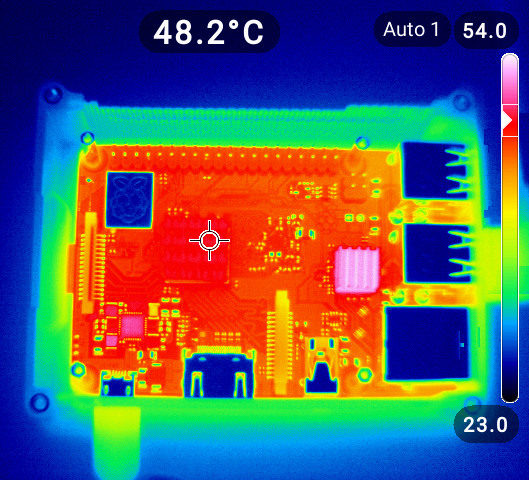
\includegraphics{images/thermal_images/RPi3Bplus_thermalImage_idleMode_c.jpg}\\
(1) Thermal image of the RPi 3B+ in idle state

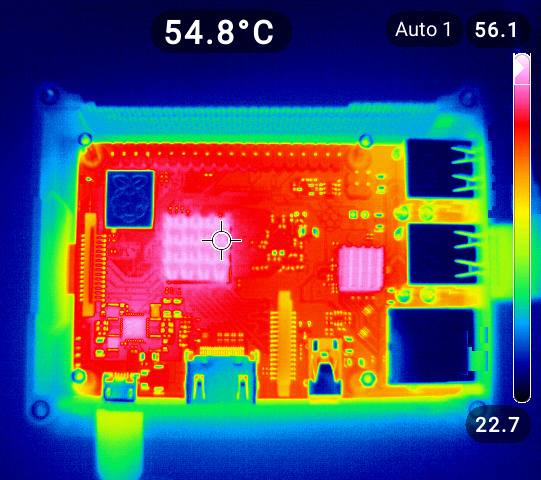
\includegraphics{images/thermal_images/RPi3Bplus_thermalImage_heavyLoadMode_c.jpg}\\
(2) Thermal image of the RPi 3B+ under CPU full load

This is the plot of the temperature curve compared with the CPU
frequency curve for the Raspberry Pi 3B+ with the cooling variant
``glued-on heat sinks without fan''.

    \begin{tcolorbox}[breakable, size=fbox, boxrule=1pt, pad at break*=1mm,colback=cellbackground, colframe=cellborder]
\prompt{In}{incolor}{9}{\boxspacing}
\begin{Verbatim}[commandchars=\\\{\}]
\PY{c+c1}{\PYZsh{} Figsize: a tuple (width, height) in inches}
\PY{c+c1}{\PYZsh{} Create figure and axis objects with subplots()}
\PY{n}{fig}\PY{p}{,} \PY{n}{ax1} \PY{o}{=} \PY{n}{plt}\PY{o}{.}\PY{n}{subplots}\PY{p}{(}\PY{n}{num}\PY{o}{=}\PY{l+m+mi}{0}\PY{p}{,} \PY{n}{figsize}\PY{o}{=}\PY{p}{(}\PY{l+m+mi}{20}\PY{p}{,} \PY{l+m+mi}{10}\PY{p}{)}\PY{p}{,} \PY{n}{dpi}\PY{o}{=}\PY{l+m+mi}{80}\PY{p}{,} \PY{n}{facecolor}\PY{o}{=}\PY{l+s+s1}{\PYZsq{}}\PY{l+s+s1}{w}\PY{l+s+s1}{\PYZsq{}}\PY{p}{,} \PY{n}{edgecolor}\PY{o}{=}\PY{l+s+s1}{\PYZsq{}}\PY{l+s+s1}{k}\PY{l+s+s1}{\PYZsq{}}\PY{p}{)}

\PY{n}{axes} \PY{o}{=} \PY{n}{plt}\PY{o}{.}\PY{n}{gca}\PY{p}{(}\PY{p}{)}

\PY{n}{plt}\PY{o}{.}\PY{n}{title}\PY{p}{(}\PY{l+s+s1}{\PYZsq{}}\PY{l+s+s1}{RaspiB3plusEPaper: passive cooling (glued\PYZhy{}on heat sinks without fan)}\PY{l+s+s1}{\PYZsq{}}\PY{p}{)}

\PY{n}{line1} \PY{o}{=} \PY{n}{ax1}\PY{o}{.}\PY{n}{plot}\PY{p}{(}\PY{n}{df\PYZus{}9\PYZus{}PC\PYZus{}wHeatSinks}\PY{p}{[}\PY{l+s+s1}{\PYZsq{}}\PY{l+s+s1}{Time}\PY{l+s+s1}{\PYZsq{}}\PY{p}{]}\PY{p}{,} \PY{n}{df\PYZus{}9\PYZus{}PC\PYZus{}wHeatSinks}\PY{p}{[}\PY{l+s+s1}{\PYZsq{}}\PY{l+s+s1}{CPU Temperature}\PY{l+s+s1}{\PYZsq{}}\PY{p}{]}\PY{p}{,} \PY{n}{color}\PY{o}{=}\PY{l+s+s1}{\PYZsq{}}\PY{l+s+s1}{navy}\PY{l+s+s1}{\PYZsq{}}\PY{p}{,} \PY{n}{label}\PY{o}{=}\PY{l+s+s1}{\PYZsq{}}\PY{l+s+s1}{CPU Temperature}\PY{l+s+s1}{\PYZsq{}}\PY{p}{)}
\PY{n}{line2} \PY{o}{=} \PY{n}{ax1}\PY{o}{.}\PY{n}{plot}\PY{p}{(}\PY{n}{df\PYZus{}9\PYZus{}PC\PYZus{}wHeatSinks}\PY{p}{[}\PY{l+s+s1}{\PYZsq{}}\PY{l+s+s1}{Time}\PY{l+s+s1}{\PYZsq{}}\PY{p}{]}\PY{p}{,} \PY{n}{df\PYZus{}9\PYZus{}PC\PYZus{}wHeatSinks}\PY{p}{[}\PY{l+s+s1}{\PYZsq{}}\PY{l+s+s1}{Ambient Temperature}\PY{l+s+s1}{\PYZsq{}}\PY{p}{]}\PY{p}{,} \PY{n}{color}\PY{o}{=}\PY{l+s+s1}{\PYZsq{}}\PY{l+s+s1}{lightseagreen}\PY{l+s+s1}{\PYZsq{}}\PY{p}{,} \PY{n}{label}\PY{o}{=}\PY{l+s+s1}{\PYZsq{}}\PY{l+s+s1}{Ambient Temperature}\PY{l+s+s1}{\PYZsq{}}\PY{p}{)}

\PY{c+c1}{\PYZsh{} Set x\PYZhy{}axis label}
\PY{n}{ax1}\PY{o}{.}\PY{n}{set\PYZus{}xlabel}\PY{p}{(}\PY{l+s+s1}{\PYZsq{}}\PY{l+s+s1}{Time [s]}\PY{l+s+s1}{\PYZsq{}}\PY{p}{,} \PY{n}{fontsize}\PY{o}{=}\PY{l+m+mi}{14}\PY{p}{)}
\PY{c+c1}{\PYZsh{} Set y\PYZhy{}axis label}
\PY{n}{ax1}\PY{o}{.}\PY{n}{set\PYZus{}ylabel}\PY{p}{(}\PY{l+s+s1}{\PYZsq{}}\PY{l+s+s1}{CPU core temperature [°C]}\PY{l+s+s1}{\PYZsq{}}\PY{p}{,} \PY{n}{fontsize}\PY{o}{=}\PY{l+m+mi}{16}\PY{p}{)}
\PY{n}{ax1}\PY{o}{.}\PY{n}{set\PYZus{}ylim}\PY{p}{(}\PY{l+m+mi}{0}\PY{p}{,} \PY{l+m+mi}{102}\PY{p}{)}
\PY{n}{ax1}\PY{o}{.}\PY{n}{grid}\PY{p}{(}\PY{k+kc}{True}\PY{p}{)}
\PY{n}{plt}\PY{o}{.}\PY{n}{xticks}\PY{p}{(}\PY{n}{rotation}\PY{o}{=}\PY{l+m+mi}{50}\PY{p}{)}

\PY{c+c1}{\PYZsh{} Twin object for two different y\PYZhy{}axis on the same plot}
\PY{n}{ax2} \PY{o}{=} \PY{n}{ax1}\PY{o}{.}\PY{n}{twinx}\PY{p}{(}\PY{p}{)}

\PY{n}{line3} \PY{o}{=} \PY{n}{ax2}\PY{o}{.}\PY{n}{plot}\PY{p}{(}\PY{n}{df\PYZus{}9\PYZus{}PC\PYZus{}wHeatSinks}\PY{p}{[}\PY{l+s+s1}{\PYZsq{}}\PY{l+s+s1}{Time}\PY{l+s+s1}{\PYZsq{}}\PY{p}{]}\PY{p}{,} \PY{n}{df\PYZus{}9\PYZus{}PC\PYZus{}wHeatSinks}\PY{p}{[}\PY{l+s+s1}{\PYZsq{}}\PY{l+s+s1}{CPU Frequency}\PY{l+s+s1}{\PYZsq{}}\PY{p}{]}\PY{p}{,} \PY{n}{color}\PY{o}{=}\PY{l+s+s1}{\PYZsq{}}\PY{l+s+s1}{limegreen}\PY{l+s+s1}{\PYZsq{}}\PY{p}{,} \PY{n}{label}\PY{o}{=}\PY{l+s+s1}{\PYZsq{}}\PY{l+s+s1}{CPU Frequency}\PY{l+s+s1}{\PYZsq{}}\PY{p}{)}

\PY{c+c1}{\PYZsh{} Set y\PYZhy{}axis label}
\PY{n}{ax2}\PY{o}{.}\PY{n}{set\PYZus{}ylabel}\PY{p}{(}\PY{l+s+s1}{\PYZsq{}}\PY{l+s+s1}{CPU core frequency [MHz]}\PY{l+s+s1}{\PYZsq{}}\PY{p}{,} \PY{n}{fontsize}\PY{o}{=}\PY{l+m+mi}{16}\PY{p}{)}
\PY{n}{ax2}\PY{o}{.}\PY{n}{set\PYZus{}ylim}\PY{p}{(}\PY{l+m+mi}{500}\PY{p}{,} \PY{l+m+mi}{1510}\PY{p}{)}
\PY{n}{ax2}\PY{o}{.}\PY{n}{grid}\PY{p}{(}\PY{k+kc}{True}\PY{p}{)}

\PY{c+c1}{\PYZsh{} Add all lines to the same legend box}
\PY{n}{lines\PYZus{}all} \PY{o}{=} \PY{n}{line1}\PY{o}{+}\PY{n}{line2}\PY{o}{+}\PY{n}{line3}
\PY{n}{labels} \PY{o}{=} \PY{p}{[}\PY{n}{l}\PY{o}{.}\PY{n}{get\PYZus{}label}\PY{p}{(}\PY{p}{)} \PY{k}{for} \PY{n}{l} \PY{o+ow}{in} \PY{n}{lines\PYZus{}all}\PY{p}{]}
\PY{n}{ax1}\PY{o}{.}\PY{n}{legend}\PY{p}{(}\PY{n}{lines\PYZus{}all}\PY{p}{,} \PY{n}{labels}\PY{p}{,} \PY{n}{loc}\PY{o}{=}\PY{l+s+s1}{\PYZsq{}}\PY{l+s+s1}{lower center}\PY{l+s+s1}{\PYZsq{}}\PY{p}{)}

\PY{c+c1}{\PYZsh{} Save plot to PNG and PDF}
\PY{n}{str\PYZus{}image\PYZus{}name} \PY{o}{=} \PY{l+s+s1}{\PYZsq{}}\PY{l+s+s1}{RaspiB3plusEPaper\PYZus{}stress\PYZus{}measurement\PYZus{}PC\PYZus{}wHeatSinks}\PY{l+s+s1}{\PYZsq{}}
\PY{c+c1}{\PYZsh{}plt.savefig(r\PYZsq{}./data\PYZus{}files/\PYZsq{} + str\PYZus{}image\PYZus{}name + \PYZsq{}.png\PYZsq{})}
\PY{n}{plt}\PY{o}{.}\PY{n}{savefig}\PY{p}{(}\PY{l+s+sa}{r}\PY{l+s+s1}{\PYZsq{}}\PY{l+s+s1}{./data\PYZus{}files/}\PY{l+s+s1}{\PYZsq{}} \PY{o}{+} \PY{n}{str\PYZus{}image\PYZus{}name} \PY{o}{+} \PY{l+s+s1}{\PYZsq{}}\PY{l+s+s1}{.pdf}\PY{l+s+s1}{\PYZsq{}}\PY{p}{)}

\PY{n}{plt}\PY{o}{.}\PY{n}{show}\PY{p}{(}\PY{p}{)}
\end{Verbatim}
\end{tcolorbox}

    \begin{center}
    \adjustimage{max size={0.9\linewidth}{0.9\paperheight}}{Raspberry_Pi4_stress_test_files/Raspberry_Pi4_stress_test_37_0.pdf}
    \end{center}
    { \hspace*{\fill} \\}
    
    \hypertarget{raspib4jupyterlab-temperature-curve-compared-with-the-curve-of-the-cpu-frequency-passive-cooling-without-heat-sinks-or-fan}{%
\subsubsection{RaspiB4JupyterLab: Temperature curve compared with the
curve of the CPU frequency (passive cooling: without heat sinks or
fan)}\label{raspib4jupyterlab-temperature-curve-compared-with-the-curve-of-the-cpu-frequency-passive-cooling-without-heat-sinks-or-fan}}

This is the plot of the temperature curve compared with the CPU
frequency curve for the Raspberry Pi B4 with the cooling variant
``passive cooling: without heat sinks or fan''.

    \begin{tcolorbox}[breakable, size=fbox, boxrule=1pt, pad at break*=1mm,colback=cellbackground, colframe=cellborder]
\prompt{In}{incolor}{10}{\boxspacing}
\begin{Verbatim}[commandchars=\\\{\}]
\PY{c+c1}{\PYZsh{} Figsize: a tuple (width, height) in inches}
\PY{c+c1}{\PYZsh{} Create figure and axis objects with subplots()}
\PY{n}{fig}\PY{p}{,} \PY{n}{ax1} \PY{o}{=} \PY{n}{plt}\PY{o}{.}\PY{n}{subplots}\PY{p}{(}\PY{n}{num}\PY{o}{=}\PY{l+m+mi}{0}\PY{p}{,} \PY{n}{figsize}\PY{o}{=}\PY{p}{(}\PY{l+m+mi}{20}\PY{p}{,} \PY{l+m+mi}{10}\PY{p}{)}\PY{p}{,} \PY{n}{dpi}\PY{o}{=}\PY{l+m+mi}{80}\PY{p}{,} \PY{n}{facecolor}\PY{o}{=}\PY{l+s+s1}{\PYZsq{}}\PY{l+s+s1}{w}\PY{l+s+s1}{\PYZsq{}}\PY{p}{,} \PY{n}{edgecolor}\PY{o}{=}\PY{l+s+s1}{\PYZsq{}}\PY{l+s+s1}{k}\PY{l+s+s1}{\PYZsq{}}\PY{p}{)}

\PY{n}{axes} \PY{o}{=} \PY{n}{plt}\PY{o}{.}\PY{n}{gca}\PY{p}{(}\PY{p}{)}

\PY{n}{plt}\PY{o}{.}\PY{n}{title}\PY{p}{(}\PY{l+s+s1}{\PYZsq{}}\PY{l+s+s1}{RaspiB4JupyterLab: passive cooling (passive cooling: without heat sinks or fan)}\PY{l+s+s1}{\PYZsq{}}\PY{p}{)}

\PY{n}{line1} \PY{o}{=} \PY{n}{ax1}\PY{o}{.}\PY{n}{plot}\PY{p}{(}\PY{n}{df\PYZus{}1\PYZus{}PC\PYZus{}woHeatSinks}\PY{p}{[}\PY{l+s+s1}{\PYZsq{}}\PY{l+s+s1}{Time}\PY{l+s+s1}{\PYZsq{}}\PY{p}{]}\PY{p}{,} \PY{n}{df\PYZus{}1\PYZus{}PC\PYZus{}woHeatSinks}\PY{p}{[}\PY{l+s+s1}{\PYZsq{}}\PY{l+s+s1}{CPU Temperature}\PY{l+s+s1}{\PYZsq{}}\PY{p}{]}\PY{p}{,} \PY{n}{color}\PY{o}{=}\PY{l+s+s1}{\PYZsq{}}\PY{l+s+s1}{navy}\PY{l+s+s1}{\PYZsq{}}\PY{p}{,} \PY{n}{label}\PY{o}{=}\PY{l+s+s1}{\PYZsq{}}\PY{l+s+s1}{CPU Temperature}\PY{l+s+s1}{\PYZsq{}}\PY{p}{)}
\PY{n}{line2} \PY{o}{=} \PY{n}{ax1}\PY{o}{.}\PY{n}{plot}\PY{p}{(}\PY{n}{df\PYZus{}1\PYZus{}PC\PYZus{}woHeatSinks}\PY{p}{[}\PY{l+s+s1}{\PYZsq{}}\PY{l+s+s1}{Time}\PY{l+s+s1}{\PYZsq{}}\PY{p}{]}\PY{p}{,} \PY{n}{df\PYZus{}1\PYZus{}PC\PYZus{}woHeatSinks}\PY{p}{[}\PY{l+s+s1}{\PYZsq{}}\PY{l+s+s1}{Ambient Temperature}\PY{l+s+s1}{\PYZsq{}}\PY{p}{]}\PY{p}{,} \PY{n}{color}\PY{o}{=}\PY{l+s+s1}{\PYZsq{}}\PY{l+s+s1}{lightseagreen}\PY{l+s+s1}{\PYZsq{}}\PY{p}{,} \PY{n}{label}\PY{o}{=}\PY{l+s+s1}{\PYZsq{}}\PY{l+s+s1}{Ambient Temperature}\PY{l+s+s1}{\PYZsq{}}\PY{p}{)}

\PY{c+c1}{\PYZsh{} Set x\PYZhy{}axis label}
\PY{n}{ax1}\PY{o}{.}\PY{n}{set\PYZus{}xlabel}\PY{p}{(}\PY{l+s+s1}{\PYZsq{}}\PY{l+s+s1}{Time [s]}\PY{l+s+s1}{\PYZsq{}}\PY{p}{,} \PY{n}{fontsize}\PY{o}{=}\PY{l+m+mi}{14}\PY{p}{)}
\PY{c+c1}{\PYZsh{} Set y\PYZhy{}axis label}
\PY{n}{ax1}\PY{o}{.}\PY{n}{set\PYZus{}ylabel}\PY{p}{(}\PY{l+s+s1}{\PYZsq{}}\PY{l+s+s1}{CPU core temperature [°C]}\PY{l+s+s1}{\PYZsq{}}\PY{p}{,} \PY{n}{fontsize}\PY{o}{=}\PY{l+m+mi}{16}\PY{p}{)}
\PY{n}{ax1}\PY{o}{.}\PY{n}{set\PYZus{}ylim}\PY{p}{(}\PY{l+m+mi}{0}\PY{p}{,} \PY{l+m+mi}{102}\PY{p}{)}
\PY{n}{ax1}\PY{o}{.}\PY{n}{grid}\PY{p}{(}\PY{k+kc}{True}\PY{p}{)}
\PY{n}{plt}\PY{o}{.}\PY{n}{xticks}\PY{p}{(}\PY{n}{rotation}\PY{o}{=}\PY{l+m+mi}{50}\PY{p}{)}

\PY{c+c1}{\PYZsh{} Twin object for two different y\PYZhy{}axis on the same plot}
\PY{n}{ax2} \PY{o}{=} \PY{n}{ax1}\PY{o}{.}\PY{n}{twinx}\PY{p}{(}\PY{p}{)}

\PY{n}{line3} \PY{o}{=} \PY{n}{ax2}\PY{o}{.}\PY{n}{plot}\PY{p}{(}\PY{n}{df\PYZus{}1\PYZus{}PC\PYZus{}woHeatSinks}\PY{p}{[}\PY{l+s+s1}{\PYZsq{}}\PY{l+s+s1}{Time}\PY{l+s+s1}{\PYZsq{}}\PY{p}{]}\PY{p}{,} \PY{n}{df\PYZus{}1\PYZus{}PC\PYZus{}woHeatSinks}\PY{p}{[}\PY{l+s+s1}{\PYZsq{}}\PY{l+s+s1}{CPU Frequency}\PY{l+s+s1}{\PYZsq{}}\PY{p}{]}\PY{p}{,} \PY{n}{color}\PY{o}{=}\PY{l+s+s1}{\PYZsq{}}\PY{l+s+s1}{limegreen}\PY{l+s+s1}{\PYZsq{}}\PY{p}{,} \PY{n}{label}\PY{o}{=}\PY{l+s+s1}{\PYZsq{}}\PY{l+s+s1}{CPU Frequency}\PY{l+s+s1}{\PYZsq{}}\PY{p}{)}

\PY{c+c1}{\PYZsh{} Set y\PYZhy{}axis label}
\PY{n}{ax2}\PY{o}{.}\PY{n}{set\PYZus{}ylabel}\PY{p}{(}\PY{l+s+s1}{\PYZsq{}}\PY{l+s+s1}{CPU core frequency [MHz]}\PY{l+s+s1}{\PYZsq{}}\PY{p}{,} \PY{n}{fontsize}\PY{o}{=}\PY{l+m+mi}{16}\PY{p}{)}
\PY{n}{ax2}\PY{o}{.}\PY{n}{set\PYZus{}ylim}\PY{p}{(}\PY{l+m+mi}{500}\PY{p}{,} \PY{l+m+mi}{1510}\PY{p}{)}
\PY{n}{ax2}\PY{o}{.}\PY{n}{grid}\PY{p}{(}\PY{k+kc}{True}\PY{p}{)}

\PY{c+c1}{\PYZsh{} Add all lines to the same legend box}
\PY{n}{lines\PYZus{}all} \PY{o}{=} \PY{n}{line1}\PY{o}{+}\PY{n}{line2}\PY{o}{+}\PY{n}{line2}
\PY{n}{labels} \PY{o}{=} \PY{p}{[}\PY{n}{l}\PY{o}{.}\PY{n}{get\PYZus{}label}\PY{p}{(}\PY{p}{)} \PY{k}{for} \PY{n}{l} \PY{o+ow}{in} \PY{n}{lines\PYZus{}all}\PY{p}{]}
\PY{n}{ax1}\PY{o}{.}\PY{n}{legend}\PY{p}{(}\PY{n}{lines\PYZus{}all}\PY{p}{,} \PY{n}{labels}\PY{p}{,} \PY{n}{loc}\PY{o}{=}\PY{l+s+s1}{\PYZsq{}}\PY{l+s+s1}{lower center}\PY{l+s+s1}{\PYZsq{}}\PY{p}{)}

\PY{c+c1}{\PYZsh{} Save plot to PNG and PDF}
\PY{n}{str\PYZus{}image\PYZus{}name} \PY{o}{=} \PY{l+s+s1}{\PYZsq{}}\PY{l+s+s1}{RaspiB4JupyterLab\PYZus{}stress\PYZus{}measurement\PYZus{}PC\PYZus{}woHeatSinks}\PY{l+s+s1}{\PYZsq{}}
\PY{c+c1}{\PYZsh{}plt.savefig(r\PYZsq{}./data\PYZus{}files/\PYZsq{} + str\PYZus{}image\PYZus{}name + \PYZsq{}.png\PYZsq{})}
\PY{n}{plt}\PY{o}{.}\PY{n}{savefig}\PY{p}{(}\PY{l+s+sa}{r}\PY{l+s+s1}{\PYZsq{}}\PY{l+s+s1}{./data\PYZus{}files/}\PY{l+s+s1}{\PYZsq{}} \PY{o}{+} \PY{n}{str\PYZus{}image\PYZus{}name} \PY{o}{+} \PY{l+s+s1}{\PYZsq{}}\PY{l+s+s1}{.pdf}\PY{l+s+s1}{\PYZsq{}}\PY{p}{)}

\PY{n}{plt}\PY{o}{.}\PY{n}{show}\PY{p}{(}\PY{p}{)}
\end{Verbatim}
\end{tcolorbox}

    \begin{center}
    \adjustimage{max size={0.9\linewidth}{0.9\paperheight}}{Raspberry_Pi4_stress_test_files/Raspberry_Pi4_stress_test_39_0.pdf}
    \end{center}
    { \hspace*{\fill} \\}
    
    \hypertarget{raspib4jupyterlab-temperature-curve-compared-with-the-curve-of-the-cpu-frequency-passive-cooling-with-heat-sinks-but-without-fan}{%
\subsubsection{RaspiB4JupyterLab: Temperature curve compared with the
curve of the CPU frequency (passive cooling: with heat sinks, but
without
fan)}\label{raspib4jupyterlab-temperature-curve-compared-with-the-curve-of-the-cpu-frequency-passive-cooling-with-heat-sinks-but-without-fan}}

This is the plot of the temperature curve compared with the CPU
frequency curve for the Raspberry Pi B4 with the cooling variant
``glued-on heat sinks without fan''.

    \begin{tcolorbox}[breakable, size=fbox, boxrule=1pt, pad at break*=1mm,colback=cellbackground, colframe=cellborder]
\prompt{In}{incolor}{11}{\boxspacing}
\begin{Verbatim}[commandchars=\\\{\}]
\PY{c+c1}{\PYZsh{} Figsize: a tuple (width, height) in inches}
\PY{c+c1}{\PYZsh{} Create figure and axis objects with subplots()}
\PY{n}{fig}\PY{p}{,} \PY{n}{ax1} \PY{o}{=} \PY{n}{plt}\PY{o}{.}\PY{n}{subplots}\PY{p}{(}\PY{n}{num}\PY{o}{=}\PY{l+m+mi}{0}\PY{p}{,} \PY{n}{figsize}\PY{o}{=}\PY{p}{(}\PY{l+m+mi}{20}\PY{p}{,} \PY{l+m+mi}{10}\PY{p}{)}\PY{p}{,} \PY{n}{dpi}\PY{o}{=}\PY{l+m+mi}{80}\PY{p}{,} \PY{n}{facecolor}\PY{o}{=}\PY{l+s+s1}{\PYZsq{}}\PY{l+s+s1}{w}\PY{l+s+s1}{\PYZsq{}}\PY{p}{,} \PY{n}{edgecolor}\PY{o}{=}\PY{l+s+s1}{\PYZsq{}}\PY{l+s+s1}{k}\PY{l+s+s1}{\PYZsq{}}\PY{p}{)}

\PY{n}{axes} \PY{o}{=} \PY{n}{plt}\PY{o}{.}\PY{n}{gca}\PY{p}{(}\PY{p}{)}

\PY{n}{plt}\PY{o}{.}\PY{n}{title}\PY{p}{(}\PY{l+s+s1}{\PYZsq{}}\PY{l+s+s1}{RaspiB4JupyterLab: passive cooling (glued\PYZhy{}on heat sinks without fan)}\PY{l+s+s1}{\PYZsq{}}\PY{p}{)}

\PY{n}{line1} \PY{o}{=} \PY{n}{ax1}\PY{o}{.}\PY{n}{plot}\PY{p}{(}\PY{n}{df\PYZus{}2\PYZus{}PC\PYZus{}wHeatSinks}\PY{p}{[}\PY{l+s+s1}{\PYZsq{}}\PY{l+s+s1}{Time}\PY{l+s+s1}{\PYZsq{}}\PY{p}{]}\PY{p}{,} \PY{n}{df\PYZus{}2\PYZus{}PC\PYZus{}wHeatSinks}\PY{p}{[}\PY{l+s+s1}{\PYZsq{}}\PY{l+s+s1}{CPU Temperature}\PY{l+s+s1}{\PYZsq{}}\PY{p}{]}\PY{p}{,} \PY{n}{color}\PY{o}{=}\PY{l+s+s1}{\PYZsq{}}\PY{l+s+s1}{navy}\PY{l+s+s1}{\PYZsq{}}\PY{p}{,} \PY{n}{label}\PY{o}{=}\PY{l+s+s1}{\PYZsq{}}\PY{l+s+s1}{CPU Temperature}\PY{l+s+s1}{\PYZsq{}}\PY{p}{)}
\PY{n}{line2} \PY{o}{=} \PY{n}{ax1}\PY{o}{.}\PY{n}{plot}\PY{p}{(}\PY{n}{df\PYZus{}2\PYZus{}PC\PYZus{}wHeatSinks}\PY{p}{[}\PY{l+s+s1}{\PYZsq{}}\PY{l+s+s1}{Time}\PY{l+s+s1}{\PYZsq{}}\PY{p}{]}\PY{p}{,} \PY{n}{df\PYZus{}2\PYZus{}PC\PYZus{}wHeatSinks}\PY{p}{[}\PY{l+s+s1}{\PYZsq{}}\PY{l+s+s1}{Ambient Temperature}\PY{l+s+s1}{\PYZsq{}}\PY{p}{]}\PY{p}{,} \PY{n}{color}\PY{o}{=}\PY{l+s+s1}{\PYZsq{}}\PY{l+s+s1}{lightseagreen}\PY{l+s+s1}{\PYZsq{}}\PY{p}{,} \PY{n}{label}\PY{o}{=}\PY{l+s+s1}{\PYZsq{}}\PY{l+s+s1}{Ambient Temperature}\PY{l+s+s1}{\PYZsq{}}\PY{p}{)}

\PY{c+c1}{\PYZsh{} Set x\PYZhy{}axis label}
\PY{n}{ax1}\PY{o}{.}\PY{n}{set\PYZus{}xlabel}\PY{p}{(}\PY{l+s+s1}{\PYZsq{}}\PY{l+s+s1}{Time [s]}\PY{l+s+s1}{\PYZsq{}}\PY{p}{,} \PY{n}{fontsize}\PY{o}{=}\PY{l+m+mi}{14}\PY{p}{)}
\PY{c+c1}{\PYZsh{} Set y\PYZhy{}axis label}
\PY{n}{ax1}\PY{o}{.}\PY{n}{set\PYZus{}ylabel}\PY{p}{(}\PY{l+s+s1}{\PYZsq{}}\PY{l+s+s1}{CPU core temperature [°C]}\PY{l+s+s1}{\PYZsq{}}\PY{p}{,} \PY{n}{fontsize}\PY{o}{=}\PY{l+m+mi}{16}\PY{p}{)}
\PY{n}{ax1}\PY{o}{.}\PY{n}{set\PYZus{}ylim}\PY{p}{(}\PY{l+m+mi}{0}\PY{p}{,} \PY{l+m+mi}{102}\PY{p}{)}
\PY{n}{ax1}\PY{o}{.}\PY{n}{grid}\PY{p}{(}\PY{k+kc}{True}\PY{p}{)}
\PY{n}{plt}\PY{o}{.}\PY{n}{xticks}\PY{p}{(}\PY{n}{rotation}\PY{o}{=}\PY{l+m+mi}{50}\PY{p}{)}

\PY{c+c1}{\PYZsh{} Twin object for two different y\PYZhy{}axis on the same plot}
\PY{n}{ax2} \PY{o}{=} \PY{n}{ax1}\PY{o}{.}\PY{n}{twinx}\PY{p}{(}\PY{p}{)}

\PY{n}{line3} \PY{o}{=} \PY{n}{ax2}\PY{o}{.}\PY{n}{plot}\PY{p}{(}\PY{n}{df\PYZus{}2\PYZus{}PC\PYZus{}wHeatSinks}\PY{p}{[}\PY{l+s+s1}{\PYZsq{}}\PY{l+s+s1}{Time}\PY{l+s+s1}{\PYZsq{}}\PY{p}{]}\PY{p}{,} \PY{n}{df\PYZus{}2\PYZus{}PC\PYZus{}wHeatSinks}\PY{p}{[}\PY{l+s+s1}{\PYZsq{}}\PY{l+s+s1}{CPU Frequency}\PY{l+s+s1}{\PYZsq{}}\PY{p}{]}\PY{p}{,} \PY{n}{color}\PY{o}{=}\PY{l+s+s1}{\PYZsq{}}\PY{l+s+s1}{limegreen}\PY{l+s+s1}{\PYZsq{}}\PY{p}{,} \PY{n}{label}\PY{o}{=}\PY{l+s+s1}{\PYZsq{}}\PY{l+s+s1}{CPU Frequency}\PY{l+s+s1}{\PYZsq{}}\PY{p}{)}

\PY{c+c1}{\PYZsh{} Set y\PYZhy{}axis label}
\PY{n}{ax2}\PY{o}{.}\PY{n}{set\PYZus{}ylabel}\PY{p}{(}\PY{l+s+s1}{\PYZsq{}}\PY{l+s+s1}{CPU core frequency [MHz]}\PY{l+s+s1}{\PYZsq{}}\PY{p}{,} \PY{n}{fontsize}\PY{o}{=}\PY{l+m+mi}{16}\PY{p}{)}
\PY{n}{ax2}\PY{o}{.}\PY{n}{set\PYZus{}ylim}\PY{p}{(}\PY{l+m+mi}{500}\PY{p}{,} \PY{l+m+mi}{1510}\PY{p}{)}
\PY{n}{ax2}\PY{o}{.}\PY{n}{grid}\PY{p}{(}\PY{k+kc}{True}\PY{p}{)}

\PY{c+c1}{\PYZsh{} Add all lines to the same legend box}
\PY{n}{lines\PYZus{}all} \PY{o}{=} \PY{n}{line1}\PY{o}{+}\PY{n}{line2}\PY{o}{+}\PY{n}{line2}
\PY{n}{labels} \PY{o}{=} \PY{p}{[}\PY{n}{l}\PY{o}{.}\PY{n}{get\PYZus{}label}\PY{p}{(}\PY{p}{)} \PY{k}{for} \PY{n}{l} \PY{o+ow}{in} \PY{n}{lines\PYZus{}all}\PY{p}{]}
\PY{n}{ax1}\PY{o}{.}\PY{n}{legend}\PY{p}{(}\PY{n}{lines\PYZus{}all}\PY{p}{,} \PY{n}{labels}\PY{p}{,} \PY{n}{loc}\PY{o}{=}\PY{l+s+s1}{\PYZsq{}}\PY{l+s+s1}{lower center}\PY{l+s+s1}{\PYZsq{}}\PY{p}{)}

\PY{c+c1}{\PYZsh{} Save plot to PNG and PDF}
\PY{n}{str\PYZus{}image\PYZus{}name} \PY{o}{=} \PY{l+s+s1}{\PYZsq{}}\PY{l+s+s1}{RaspiB4JupyterLab\PYZus{}stress\PYZus{}measurement\PYZus{}PC\PYZus{}wHeatSinks}\PY{l+s+s1}{\PYZsq{}}
\PY{c+c1}{\PYZsh{}plt.savefig(r\PYZsq{}./data\PYZus{}files/\PYZsq{} + str\PYZus{}image\PYZus{}name + \PYZsq{}.png\PYZsq{})}
\PY{n}{plt}\PY{o}{.}\PY{n}{savefig}\PY{p}{(}\PY{l+s+sa}{r}\PY{l+s+s1}{\PYZsq{}}\PY{l+s+s1}{./data\PYZus{}files/}\PY{l+s+s1}{\PYZsq{}} \PY{o}{+} \PY{n}{str\PYZus{}image\PYZus{}name} \PY{o}{+} \PY{l+s+s1}{\PYZsq{}}\PY{l+s+s1}{.pdf}\PY{l+s+s1}{\PYZsq{}}\PY{p}{)}

\PY{n}{plt}\PY{o}{.}\PY{n}{show}\PY{p}{(}\PY{p}{)}
\end{Verbatim}
\end{tcolorbox}

    \begin{center}
    \adjustimage{max size={0.9\linewidth}{0.9\paperheight}}{Raspberry_Pi4_stress_test_files/Raspberry_Pi4_stress_test_41_0.pdf}
    \end{center}
    { \hspace*{\fill} \\}
    
    \hypertarget{raspib4jupyterlab-temperature-curve-compared-with-the-curve-of-the-cpu-frequency-active-cooling}{%
\subsubsection{RaspiB4JupyterLab: Temperature curve compared with the
curve of the CPU frequency (active
cooling)}\label{raspib4jupyterlab-temperature-curve-compared-with-the-curve-of-the-cpu-frequency-active-cooling}}

This is the plot of the temperature curve compared with the CPU
frequency curve for the Raspberry Pi B4 with the cooling variant
``glued-on heat sinks with Noctua fan (driven by 3.3 V)''.

    \begin{tcolorbox}[breakable, size=fbox, boxrule=1pt, pad at break*=1mm,colback=cellbackground, colframe=cellborder]
\prompt{In}{incolor}{12}{\boxspacing}
\begin{Verbatim}[commandchars=\\\{\}]
\PY{c+c1}{\PYZsh{} Figsize: a tuple (width, height) in inches}
\PY{c+c1}{\PYZsh{} Create figure and axis objects with subplots()}
\PY{n}{fig}\PY{p}{,} \PY{n}{ax1} \PY{o}{=} \PY{n}{plt}\PY{o}{.}\PY{n}{subplots}\PY{p}{(}\PY{n}{num}\PY{o}{=}\PY{l+m+mi}{0}\PY{p}{,} \PY{n}{figsize}\PY{o}{=}\PY{p}{(}\PY{l+m+mi}{20}\PY{p}{,} \PY{l+m+mi}{10}\PY{p}{)}\PY{p}{,} \PY{n}{dpi}\PY{o}{=}\PY{l+m+mi}{80}\PY{p}{,} \PY{n}{facecolor}\PY{o}{=}\PY{l+s+s1}{\PYZsq{}}\PY{l+s+s1}{w}\PY{l+s+s1}{\PYZsq{}}\PY{p}{,} \PY{n}{edgecolor}\PY{o}{=}\PY{l+s+s1}{\PYZsq{}}\PY{l+s+s1}{k}\PY{l+s+s1}{\PYZsq{}}\PY{p}{)}

\PY{n}{axes} \PY{o}{=} \PY{n}{plt}\PY{o}{.}\PY{n}{gca}\PY{p}{(}\PY{p}{)}

\PY{n}{plt}\PY{o}{.}\PY{n}{title}\PY{p}{(}\PY{l+s+s1}{\PYZsq{}}\PY{l+s+s1}{RaspiB4JupyterLab: active cooling (glued\PYZhy{}on heat sinks with Noctua fan, 3.3 V)}\PY{l+s+s1}{\PYZsq{}}\PY{p}{)}

\PY{n}{line1} \PY{o}{=} \PY{n}{ax1}\PY{o}{.}\PY{n}{plot}\PY{p}{(}\PY{n}{df\PYZus{}8\PYZus{}PC\PYZus{}wHeatSinksAndNoctuaFan3V}\PY{p}{[}\PY{l+s+s1}{\PYZsq{}}\PY{l+s+s1}{Time}\PY{l+s+s1}{\PYZsq{}}\PY{p}{]}\PY{p}{,} \PY{n}{df\PYZus{}8\PYZus{}PC\PYZus{}wHeatSinksAndNoctuaFan3V}\PY{p}{[}\PY{l+s+s1}{\PYZsq{}}\PY{l+s+s1}{CPU Temperature}\PY{l+s+s1}{\PYZsq{}}\PY{p}{]}\PY{p}{,} \PY{n}{color}\PY{o}{=}\PY{l+s+s1}{\PYZsq{}}\PY{l+s+s1}{navy}\PY{l+s+s1}{\PYZsq{}}\PY{p}{,} \PY{n}{label}\PY{o}{=}\PY{l+s+s1}{\PYZsq{}}\PY{l+s+s1}{CPU Temperature}\PY{l+s+s1}{\PYZsq{}}\PY{p}{)}
\PY{n}{line2} \PY{o}{=} \PY{n}{ax1}\PY{o}{.}\PY{n}{plot}\PY{p}{(}\PY{n}{df\PYZus{}8\PYZus{}PC\PYZus{}wHeatSinksAndNoctuaFan3V}\PY{p}{[}\PY{l+s+s1}{\PYZsq{}}\PY{l+s+s1}{Time}\PY{l+s+s1}{\PYZsq{}}\PY{p}{]}\PY{p}{,} \PY{n}{df\PYZus{}8\PYZus{}PC\PYZus{}wHeatSinksAndNoctuaFan3V}\PY{p}{[}\PY{l+s+s1}{\PYZsq{}}\PY{l+s+s1}{Ambient Temperature}\PY{l+s+s1}{\PYZsq{}}\PY{p}{]}\PY{p}{,} \PY{n}{color}\PY{o}{=}\PY{l+s+s1}{\PYZsq{}}\PY{l+s+s1}{lightseagreen}\PY{l+s+s1}{\PYZsq{}}\PY{p}{,} \PY{n}{label}\PY{o}{=}\PY{l+s+s1}{\PYZsq{}}\PY{l+s+s1}{Ambient Temperature}\PY{l+s+s1}{\PYZsq{}}\PY{p}{)}

\PY{c+c1}{\PYZsh{} Set x\PYZhy{}axis label}
\PY{n}{ax1}\PY{o}{.}\PY{n}{set\PYZus{}xlabel}\PY{p}{(}\PY{l+s+s1}{\PYZsq{}}\PY{l+s+s1}{Time [s]}\PY{l+s+s1}{\PYZsq{}}\PY{p}{,} \PY{n}{fontsize}\PY{o}{=}\PY{l+m+mi}{14}\PY{p}{)}
\PY{c+c1}{\PYZsh{} Set y\PYZhy{}axis label}
\PY{n}{ax1}\PY{o}{.}\PY{n}{set\PYZus{}ylabel}\PY{p}{(}\PY{l+s+s1}{\PYZsq{}}\PY{l+s+s1}{CPU core temperature [°C]}\PY{l+s+s1}{\PYZsq{}}\PY{p}{,} \PY{n}{fontsize}\PY{o}{=}\PY{l+m+mi}{16}\PY{p}{)}
\PY{n}{ax1}\PY{o}{.}\PY{n}{set\PYZus{}ylim}\PY{p}{(}\PY{l+m+mi}{0}\PY{p}{,} \PY{l+m+mi}{102}\PY{p}{)}
\PY{n}{ax1}\PY{o}{.}\PY{n}{grid}\PY{p}{(}\PY{k+kc}{True}\PY{p}{)}
\PY{n}{plt}\PY{o}{.}\PY{n}{xticks}\PY{p}{(}\PY{n}{rotation}\PY{o}{=}\PY{l+m+mi}{50}\PY{p}{)}

\PY{c+c1}{\PYZsh{} Twin object for two different y\PYZhy{}axis on the same plot}
\PY{n}{ax2} \PY{o}{=} \PY{n}{ax1}\PY{o}{.}\PY{n}{twinx}\PY{p}{(}\PY{p}{)}

\PY{n}{line3} \PY{o}{=} \PY{n}{ax2}\PY{o}{.}\PY{n}{plot}\PY{p}{(}\PY{n}{df\PYZus{}8\PYZus{}PC\PYZus{}wHeatSinksAndNoctuaFan3V}\PY{p}{[}\PY{l+s+s1}{\PYZsq{}}\PY{l+s+s1}{Time}\PY{l+s+s1}{\PYZsq{}}\PY{p}{]}\PY{p}{,} \PY{n}{df\PYZus{}8\PYZus{}PC\PYZus{}wHeatSinksAndNoctuaFan3V}\PY{p}{[}\PY{l+s+s1}{\PYZsq{}}\PY{l+s+s1}{CPU Frequency}\PY{l+s+s1}{\PYZsq{}}\PY{p}{]}\PY{p}{,} \PY{n}{color}\PY{o}{=}\PY{l+s+s1}{\PYZsq{}}\PY{l+s+s1}{limegreen}\PY{l+s+s1}{\PYZsq{}}\PY{p}{,} \PY{n}{label}\PY{o}{=}\PY{l+s+s1}{\PYZsq{}}\PY{l+s+s1}{CPU Frequency}\PY{l+s+s1}{\PYZsq{}}\PY{p}{)}

\PY{c+c1}{\PYZsh{} Set y\PYZhy{}axis label}
\PY{n}{ax2}\PY{o}{.}\PY{n}{set\PYZus{}ylabel}\PY{p}{(}\PY{l+s+s1}{\PYZsq{}}\PY{l+s+s1}{CPU core frequency [MHz]}\PY{l+s+s1}{\PYZsq{}}\PY{p}{,} \PY{n}{fontsize}\PY{o}{=}\PY{l+m+mi}{16}\PY{p}{)}
\PY{n}{ax2}\PY{o}{.}\PY{n}{set\PYZus{}ylim}\PY{p}{(}\PY{l+m+mi}{500}\PY{p}{,} \PY{l+m+mi}{1510}\PY{p}{)}
\PY{n}{ax2}\PY{o}{.}\PY{n}{grid}\PY{p}{(}\PY{k+kc}{True}\PY{p}{)}

\PY{c+c1}{\PYZsh{} Add all lines to the same legend box}
\PY{n}{lines\PYZus{}all} \PY{o}{=} \PY{n}{line1}\PY{o}{+}\PY{n}{line2}\PY{o}{+}\PY{n}{line3}
\PY{n}{labels} \PY{o}{=} \PY{p}{[}\PY{n}{l}\PY{o}{.}\PY{n}{get\PYZus{}label}\PY{p}{(}\PY{p}{)} \PY{k}{for} \PY{n}{l} \PY{o+ow}{in} \PY{n}{lines\PYZus{}all}\PY{p}{]}
\PY{n}{ax1}\PY{o}{.}\PY{n}{legend}\PY{p}{(}\PY{n}{lines\PYZus{}all}\PY{p}{,} \PY{n}{labels}\PY{p}{,} \PY{n}{loc}\PY{o}{=}\PY{l+s+s1}{\PYZsq{}}\PY{l+s+s1}{lower center}\PY{l+s+s1}{\PYZsq{}}\PY{p}{)}

\PY{c+c1}{\PYZsh{} Save plot to PNG and PDF}
\PY{n}{str\PYZus{}image\PYZus{}name} \PY{o}{=} \PY{l+s+s1}{\PYZsq{}}\PY{l+s+s1}{RaspiB4JupyterLab\PYZus{}stress\PYZus{}measurement\PYZus{}PC\PYZus{}wHeatSinksAndNoctuaFan3V}\PY{l+s+s1}{\PYZsq{}}
\PY{c+c1}{\PYZsh{}plt.savefig(r\PYZsq{}./data\PYZus{}files/\PYZsq{} + str\PYZus{}image\PYZus{}name + \PYZsq{}.png\PYZsq{})}
\PY{n}{plt}\PY{o}{.}\PY{n}{savefig}\PY{p}{(}\PY{l+s+sa}{r}\PY{l+s+s1}{\PYZsq{}}\PY{l+s+s1}{./data\PYZus{}files/}\PY{l+s+s1}{\PYZsq{}} \PY{o}{+} \PY{n}{str\PYZus{}image\PYZus{}name} \PY{o}{+} \PY{l+s+s1}{\PYZsq{}}\PY{l+s+s1}{.pdf}\PY{l+s+s1}{\PYZsq{}}\PY{p}{)}

\PY{n}{plt}\PY{o}{.}\PY{n}{show}\PY{p}{(}\PY{p}{)}
\end{Verbatim}
\end{tcolorbox}

    \begin{center}
    \adjustimage{max size={0.9\linewidth}{0.9\paperheight}}{Raspberry_Pi4_stress_test_files/Raspberry_Pi4_stress_test_43_0.pdf}
    \end{center}
    { \hspace*{\fill} \\}
    
    \hypertarget{raspib4jupyterlab-temperature-curve-compared-with-the-curve-of-the-cpu-frequency-active-cooling-by-controlled-fan}{%
\subsubsection{RaspiB4JupyterLab: Temperature curve compared with the
curve of the CPU frequency (active cooling by controlled
fan)}\label{raspib4jupyterlab-temperature-curve-compared-with-the-curve-of-the-cpu-frequency-active-cooling-by-controlled-fan}}

The following thermal images show the \textbf{Raspberry Pi 4B} in idle
(1) state and under CPU full load (2). The images were taken with the
thermal camera \emph{Ti 480 Thermal Imager (Fluke)}:

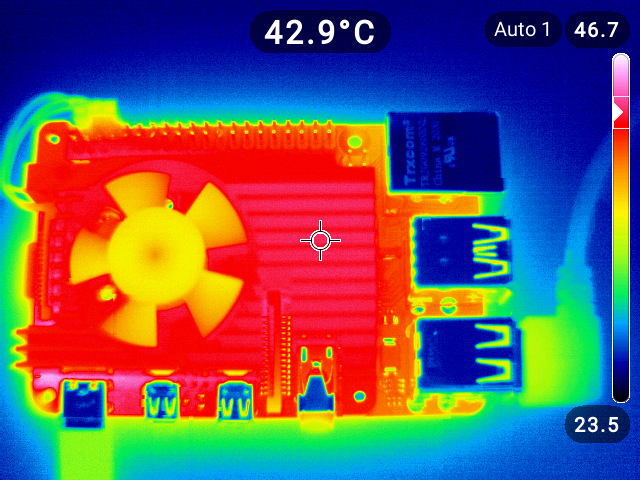
\includegraphics{images/thermal_images/RPi4_thermalImage_idleMode_wHeatSinkAndCtrlFan5V.jpg}\\
(1) Thermal image of the RPi 4B in idle state

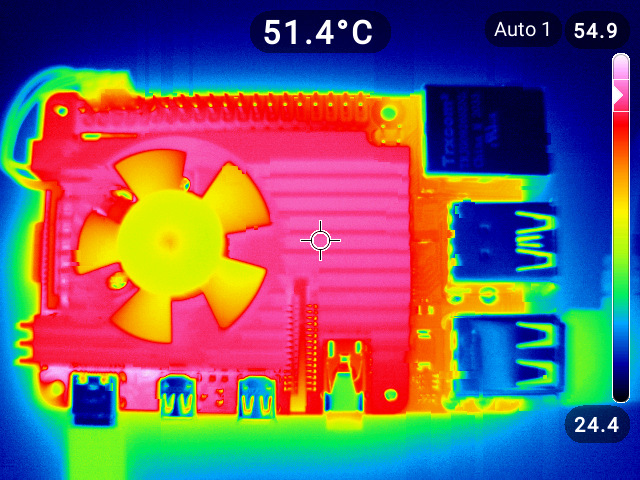
\includegraphics{images/thermal_images/RPi4_thermalImage_heavyLoadMode_wHeatSinkAndCtrlFan5V.jpg}\\
(2) Thermal image of the RPi 4B under CPU full load

This is the plot of the temperature curve compared with the CPU
frequency curve for the Raspberry Pi B4 with the cooling variant ``wo
Case and one big heat sink with controlled fan (driven by 5 V and 65°C
switch-on temperature)''.

    \begin{tcolorbox}[breakable, size=fbox, boxrule=1pt, pad at break*=1mm,colback=cellbackground, colframe=cellborder]
\prompt{In}{incolor}{15}{\boxspacing}
\begin{Verbatim}[commandchars=\\\{\}]
\PY{c+c1}{\PYZsh{} Figsize: a tuple (width, height) in inches}
\PY{c+c1}{\PYZsh{} Create figure and axis objects with subplots()}
\PY{n}{fig}\PY{p}{,} \PY{n}{ax1} \PY{o}{=} \PY{n}{plt}\PY{o}{.}\PY{n}{subplots}\PY{p}{(}\PY{n}{num}\PY{o}{=}\PY{l+m+mi}{0}\PY{p}{,} \PY{n}{figsize}\PY{o}{=}\PY{p}{(}\PY{l+m+mi}{20}\PY{p}{,} \PY{l+m+mi}{10}\PY{p}{)}\PY{p}{,} \PY{n}{dpi}\PY{o}{=}\PY{l+m+mi}{80}\PY{p}{,} \PY{n}{facecolor}\PY{o}{=}\PY{l+s+s1}{\PYZsq{}}\PY{l+s+s1}{w}\PY{l+s+s1}{\PYZsq{}}\PY{p}{,} \PY{n}{edgecolor}\PY{o}{=}\PY{l+s+s1}{\PYZsq{}}\PY{l+s+s1}{k}\PY{l+s+s1}{\PYZsq{}}\PY{p}{)}

\PY{n}{axes} \PY{o}{=} \PY{n}{plt}\PY{o}{.}\PY{n}{gca}\PY{p}{(}\PY{p}{)}

\PY{n}{plt}\PY{o}{.}\PY{n}{title}\PY{p}{(}\PY{l+s+s1}{\PYZsq{}}\PY{l+s+s1}{RaspiB4JupyterLab: active cooling (wo Case and one big heat sink with controlled fan, 5 V, 65°C switch\PYZhy{}on temperature)}\PY{l+s+s1}{\PYZsq{}}\PY{p}{)}

\PY{c+c1}{\PYZsh{} List of named colors: https://matplotlib.org/stable/gallery/color/named\PYZus{}colors.html}
\PY{n}{line1} \PY{o}{=} \PY{n}{ax1}\PY{o}{.}\PY{n}{plot}\PY{p}{(}\PY{n}{df\PYZus{}12\PYZus{}woC\PYZus{}wHeatSinksAndCtrlFan5V\PYZus{}65C}\PY{p}{[}\PY{l+s+s1}{\PYZsq{}}\PY{l+s+s1}{Time}\PY{l+s+s1}{\PYZsq{}}\PY{p}{]}\PY{p}{,} \PY{n}{df\PYZus{}12\PYZus{}woC\PYZus{}wHeatSinksAndCtrlFan5V\PYZus{}65C}\PY{p}{[}\PY{l+s+s1}{\PYZsq{}}\PY{l+s+s1}{CPU Temperature}\PY{l+s+s1}{\PYZsq{}}\PY{p}{]}\PY{p}{,} \PY{n}{color}\PY{o}{=}\PY{l+s+s1}{\PYZsq{}}\PY{l+s+s1}{navy}\PY{l+s+s1}{\PYZsq{}}\PY{p}{,} \PY{n}{label}\PY{o}{=}\PY{l+s+s1}{\PYZsq{}}\PY{l+s+s1}{CPU Temperature}\PY{l+s+s1}{\PYZsq{}}\PY{p}{)}
\PY{n}{line2} \PY{o}{=} \PY{n}{ax1}\PY{o}{.}\PY{n}{plot}\PY{p}{(}\PY{n}{df\PYZus{}12\PYZus{}woC\PYZus{}wHeatSinksAndCtrlFan5V\PYZus{}65C}\PY{p}{[}\PY{l+s+s1}{\PYZsq{}}\PY{l+s+s1}{Time}\PY{l+s+s1}{\PYZsq{}}\PY{p}{]}\PY{p}{,} \PY{n}{df\PYZus{}12\PYZus{}woC\PYZus{}wHeatSinksAndCtrlFan5V\PYZus{}65C}\PY{p}{[}\PY{l+s+s1}{\PYZsq{}}\PY{l+s+s1}{Ambient Temperature}\PY{l+s+s1}{\PYZsq{}}\PY{p}{]}\PY{p}{,} \PY{n}{color}\PY{o}{=}\PY{l+s+s1}{\PYZsq{}}\PY{l+s+s1}{lightseagreen}\PY{l+s+s1}{\PYZsq{}}\PY{p}{,} \PY{n}{label}\PY{o}{=}\PY{l+s+s1}{\PYZsq{}}\PY{l+s+s1}{Ambient Temperature}\PY{l+s+s1}{\PYZsq{}}\PY{p}{)}

\PY{c+c1}{\PYZsh{}df\PYZus{}10\PYZus{}woC\PYZus{}wHeatSinksAndCtrlFan5V\PYZus{}70C}
\PY{c+c1}{\PYZsh{}df\PYZus{}12\PYZus{}woC\PYZus{}wHeatSinksAndCtrlFan5V\PYZus{}65C}

\PY{c+c1}{\PYZsh{} Set x\PYZhy{}axis label}
\PY{n}{ax1}\PY{o}{.}\PY{n}{set\PYZus{}xlabel}\PY{p}{(}\PY{l+s+s1}{\PYZsq{}}\PY{l+s+s1}{Time [s]}\PY{l+s+s1}{\PYZsq{}}\PY{p}{,} \PY{n}{fontsize}\PY{o}{=}\PY{l+m+mi}{14}\PY{p}{)}
\PY{c+c1}{\PYZsh{} Set y\PYZhy{}axis label}
\PY{n}{ax1}\PY{o}{.}\PY{n}{set\PYZus{}ylabel}\PY{p}{(}\PY{l+s+s1}{\PYZsq{}}\PY{l+s+s1}{CPU core temperature [°C]}\PY{l+s+s1}{\PYZsq{}}\PY{p}{,} \PY{n}{fontsize}\PY{o}{=}\PY{l+m+mi}{16}\PY{p}{)}
\PY{n}{ax1}\PY{o}{.}\PY{n}{set\PYZus{}ylim}\PY{p}{(}\PY{l+m+mi}{0}\PY{p}{,} \PY{l+m+mi}{102}\PY{p}{)}
\PY{n}{ax1}\PY{o}{.}\PY{n}{grid}\PY{p}{(}\PY{k+kc}{True}\PY{p}{)}
\PY{n}{plt}\PY{o}{.}\PY{n}{xticks}\PY{p}{(}\PY{n}{rotation}\PY{o}{=}\PY{l+m+mi}{50}\PY{p}{)}

\PY{c+c1}{\PYZsh{} Twin object for two different y\PYZhy{}axis on the same plot}
\PY{n}{ax2} \PY{o}{=} \PY{n}{ax1}\PY{o}{.}\PY{n}{twinx}\PY{p}{(}\PY{p}{)}

\PY{n}{line3} \PY{o}{=} \PY{n}{ax2}\PY{o}{.}\PY{n}{plot}\PY{p}{(}\PY{n}{df\PYZus{}12\PYZus{}woC\PYZus{}wHeatSinksAndCtrlFan5V\PYZus{}65C}\PY{p}{[}\PY{l+s+s1}{\PYZsq{}}\PY{l+s+s1}{Time}\PY{l+s+s1}{\PYZsq{}}\PY{p}{]}\PY{p}{,} \PY{n}{df\PYZus{}12\PYZus{}woC\PYZus{}wHeatSinksAndCtrlFan5V\PYZus{}65C}\PY{p}{[}\PY{l+s+s1}{\PYZsq{}}\PY{l+s+s1}{CPU Frequency}\PY{l+s+s1}{\PYZsq{}}\PY{p}{]}\PY{p}{,} \PY{n}{color}\PY{o}{=}\PY{l+s+s1}{\PYZsq{}}\PY{l+s+s1}{limegreen}\PY{l+s+s1}{\PYZsq{}}\PY{p}{,} \PY{n}{label}\PY{o}{=}\PY{l+s+s1}{\PYZsq{}}\PY{l+s+s1}{CPU Frequency}\PY{l+s+s1}{\PYZsq{}}\PY{p}{)}

\PY{c+c1}{\PYZsh{} Set y\PYZhy{}axis label}
\PY{n}{ax2}\PY{o}{.}\PY{n}{set\PYZus{}ylabel}\PY{p}{(}\PY{l+s+s1}{\PYZsq{}}\PY{l+s+s1}{CPU core frequency [MHz]}\PY{l+s+s1}{\PYZsq{}}\PY{p}{,} \PY{n}{fontsize}\PY{o}{=}\PY{l+m+mi}{16}\PY{p}{)}
\PY{n}{ax2}\PY{o}{.}\PY{n}{set\PYZus{}ylim}\PY{p}{(}\PY{l+m+mi}{500}\PY{p}{,} \PY{l+m+mi}{1510}\PY{p}{)}
\PY{n}{ax2}\PY{o}{.}\PY{n}{grid}\PY{p}{(}\PY{k+kc}{True}\PY{p}{)}

\PY{c+c1}{\PYZsh{} Add all lines to the same legend box}
\PY{n}{lines\PYZus{}all} \PY{o}{=} \PY{n}{line1}\PY{o}{+}\PY{n}{line2}\PY{o}{+}\PY{n}{line3}
\PY{n}{labels} \PY{o}{=} \PY{p}{[}\PY{n}{l}\PY{o}{.}\PY{n}{get\PYZus{}label}\PY{p}{(}\PY{p}{)} \PY{k}{for} \PY{n}{l} \PY{o+ow}{in} \PY{n}{lines\PYZus{}all}\PY{p}{]}
\PY{n}{ax1}\PY{o}{.}\PY{n}{legend}\PY{p}{(}\PY{n}{lines\PYZus{}all}\PY{p}{,} \PY{n}{labels}\PY{p}{,} \PY{n}{loc}\PY{o}{=}\PY{l+s+s1}{\PYZsq{}}\PY{l+s+s1}{lower center}\PY{l+s+s1}{\PYZsq{}}\PY{p}{)}

\PY{c+c1}{\PYZsh{} Save plot to PNG and PDF}
\PY{n}{str\PYZus{}image\PYZus{}name} \PY{o}{=} \PY{l+s+s1}{\PYZsq{}}\PY{l+s+s1}{RaspiB4JupyterLab\PYZus{}stress\PYZus{}measurement\PYZus{}woCase\PYZus{}wHeatSinksAndCtrlFan5V\PYZus{}65C}\PY{l+s+s1}{\PYZsq{}}
\PY{c+c1}{\PYZsh{}plt.savefig(r\PYZsq{}./data\PYZus{}files/\PYZsq{} + str\PYZus{}image\PYZus{}name + \PYZsq{}.png\PYZsq{})}
\PY{n}{plt}\PY{o}{.}\PY{n}{savefig}\PY{p}{(}\PY{l+s+sa}{r}\PY{l+s+s1}{\PYZsq{}}\PY{l+s+s1}{./data\PYZus{}files/}\PY{l+s+s1}{\PYZsq{}} \PY{o}{+} \PY{n}{str\PYZus{}image\PYZus{}name} \PY{o}{+} \PY{l+s+s1}{\PYZsq{}}\PY{l+s+s1}{.pdf}\PY{l+s+s1}{\PYZsq{}}\PY{p}{)}

\PY{n}{plt}\PY{o}{.}\PY{n}{show}\PY{p}{(}\PY{p}{)}
\end{Verbatim}
\end{tcolorbox}

    \begin{center}
    \adjustimage{max size={0.9\linewidth}{0.9\paperheight}}{Raspberry_Pi4_stress_test_files/Raspberry_Pi4_stress_test_45_0.pdf}
    \end{center}
    { \hspace*{\fill} \\}
    
    \begin{tcolorbox}[breakable, size=fbox, boxrule=1pt, pad at break*=1mm,colback=cellbackground, colframe=cellborder]
\prompt{In}{incolor}{ }{\boxspacing}
\begin{Verbatim}[commandchars=\\\{\}]

\end{Verbatim}
\end{tcolorbox}


    % Add a bibliography block to the postdoc
    
    
    
\end{document}
